\documentclass[11pt]{article}
\usepackage[margin=0.75in]{geometry}
\usepackage{graphicx}
\usepackage{float}
\usepackage{booktabs}
\usepackage{multirow}
\usepackage{array}
\usepackage{fancyhdr}
\usepackage{titlesec}
\usepackage{amsmath}
\usepackage{amsfonts}
\usepackage{url}
\usepackage{hyperref}
\usepackage{xcolor}
\usepackage{caption}
\usepackage{subcaption}

% Page setup
\pagestyle{fancy}
\fancyhf{}
\rfoot{\thepage}
\renewcommand{\headrulewidth}{0pt}

% Section formatting
\titleformat{\section}{\large\bfseries}{\thesection}{1em}{}
\titleformat{\subsection}{\normalsize\bfseries}{\thesubsection}{1em}{}

% Custom colors
\definecolor{darkblue}{RGB}{0,0,139}
\definecolor{darkred}{RGB}{139,0,0}

% Improve text justification
\usepackage{microtype}
\setlength{\parindent}{0pt}
\setlength{\parskip}{6pt}
\usepackage{ragged2e}
\justifying

\begin{document}

% Cover Page
\begin{titlepage}
\centering
\vspace*{2cm}

{\Huge\bfseries Beauty Consumption vs. Disposable Income}\\[0.5cm]
{\Large Investment Analysis for Emerging Market Opportunities}\\[1.5cm]

\vspace{2cm}

{\large
\textbf{Executive Summary \& Strategic Assessment}\\[0.3cm]
Statistical Analysis of Income Thresholds and Growth Patterns\\[0.3cm]
Across Global Beauty Markets
}

\vspace{3cm}

{\Large
\textbf{Arnav Jaitly}\\[0.5cm]
August 2025
}

\vfill

\end{titlepage}

\newpage

% Executive Summary
\section*{Executive Summary}
\addcontentsline{toc}{section}{Executive Summary}

This report analyzes beauty consumption across 11 countries to evaluate emerging market opportunities, focusing on India's potential. We examine whether beauty consumption accelerates at income thresholds and assess India versus successful peers. Beauty markets expand 2x faster than the economy once thresholds are reached, with predictable acceleration points enabling strategic timing.

\textbf{Key Findings:}
\vspace{-3pt}
\begin{itemize}
    \setlength{\itemsep}{1pt}
    \item \textbf{Beauty as luxury}: 10\% income increase drives 23\% beauty spending growth
    \item \textbf{Clear threshold}: Markets accelerate at \$40-50k GDP per capita
    \item \textbf{India's gap}: 4.1\% growth vs 15-35\% by comparable markets
    \item \textbf{Strategic categories}: Skincare and women's beauty show strongest acceleration
    \item \textbf{Catalyst opportunity}: Countries can break through thresholds earlier
\end{itemize}

\begin{figure}[H]
\centering
\begin{subfigure}[b]{0.48\textwidth}
    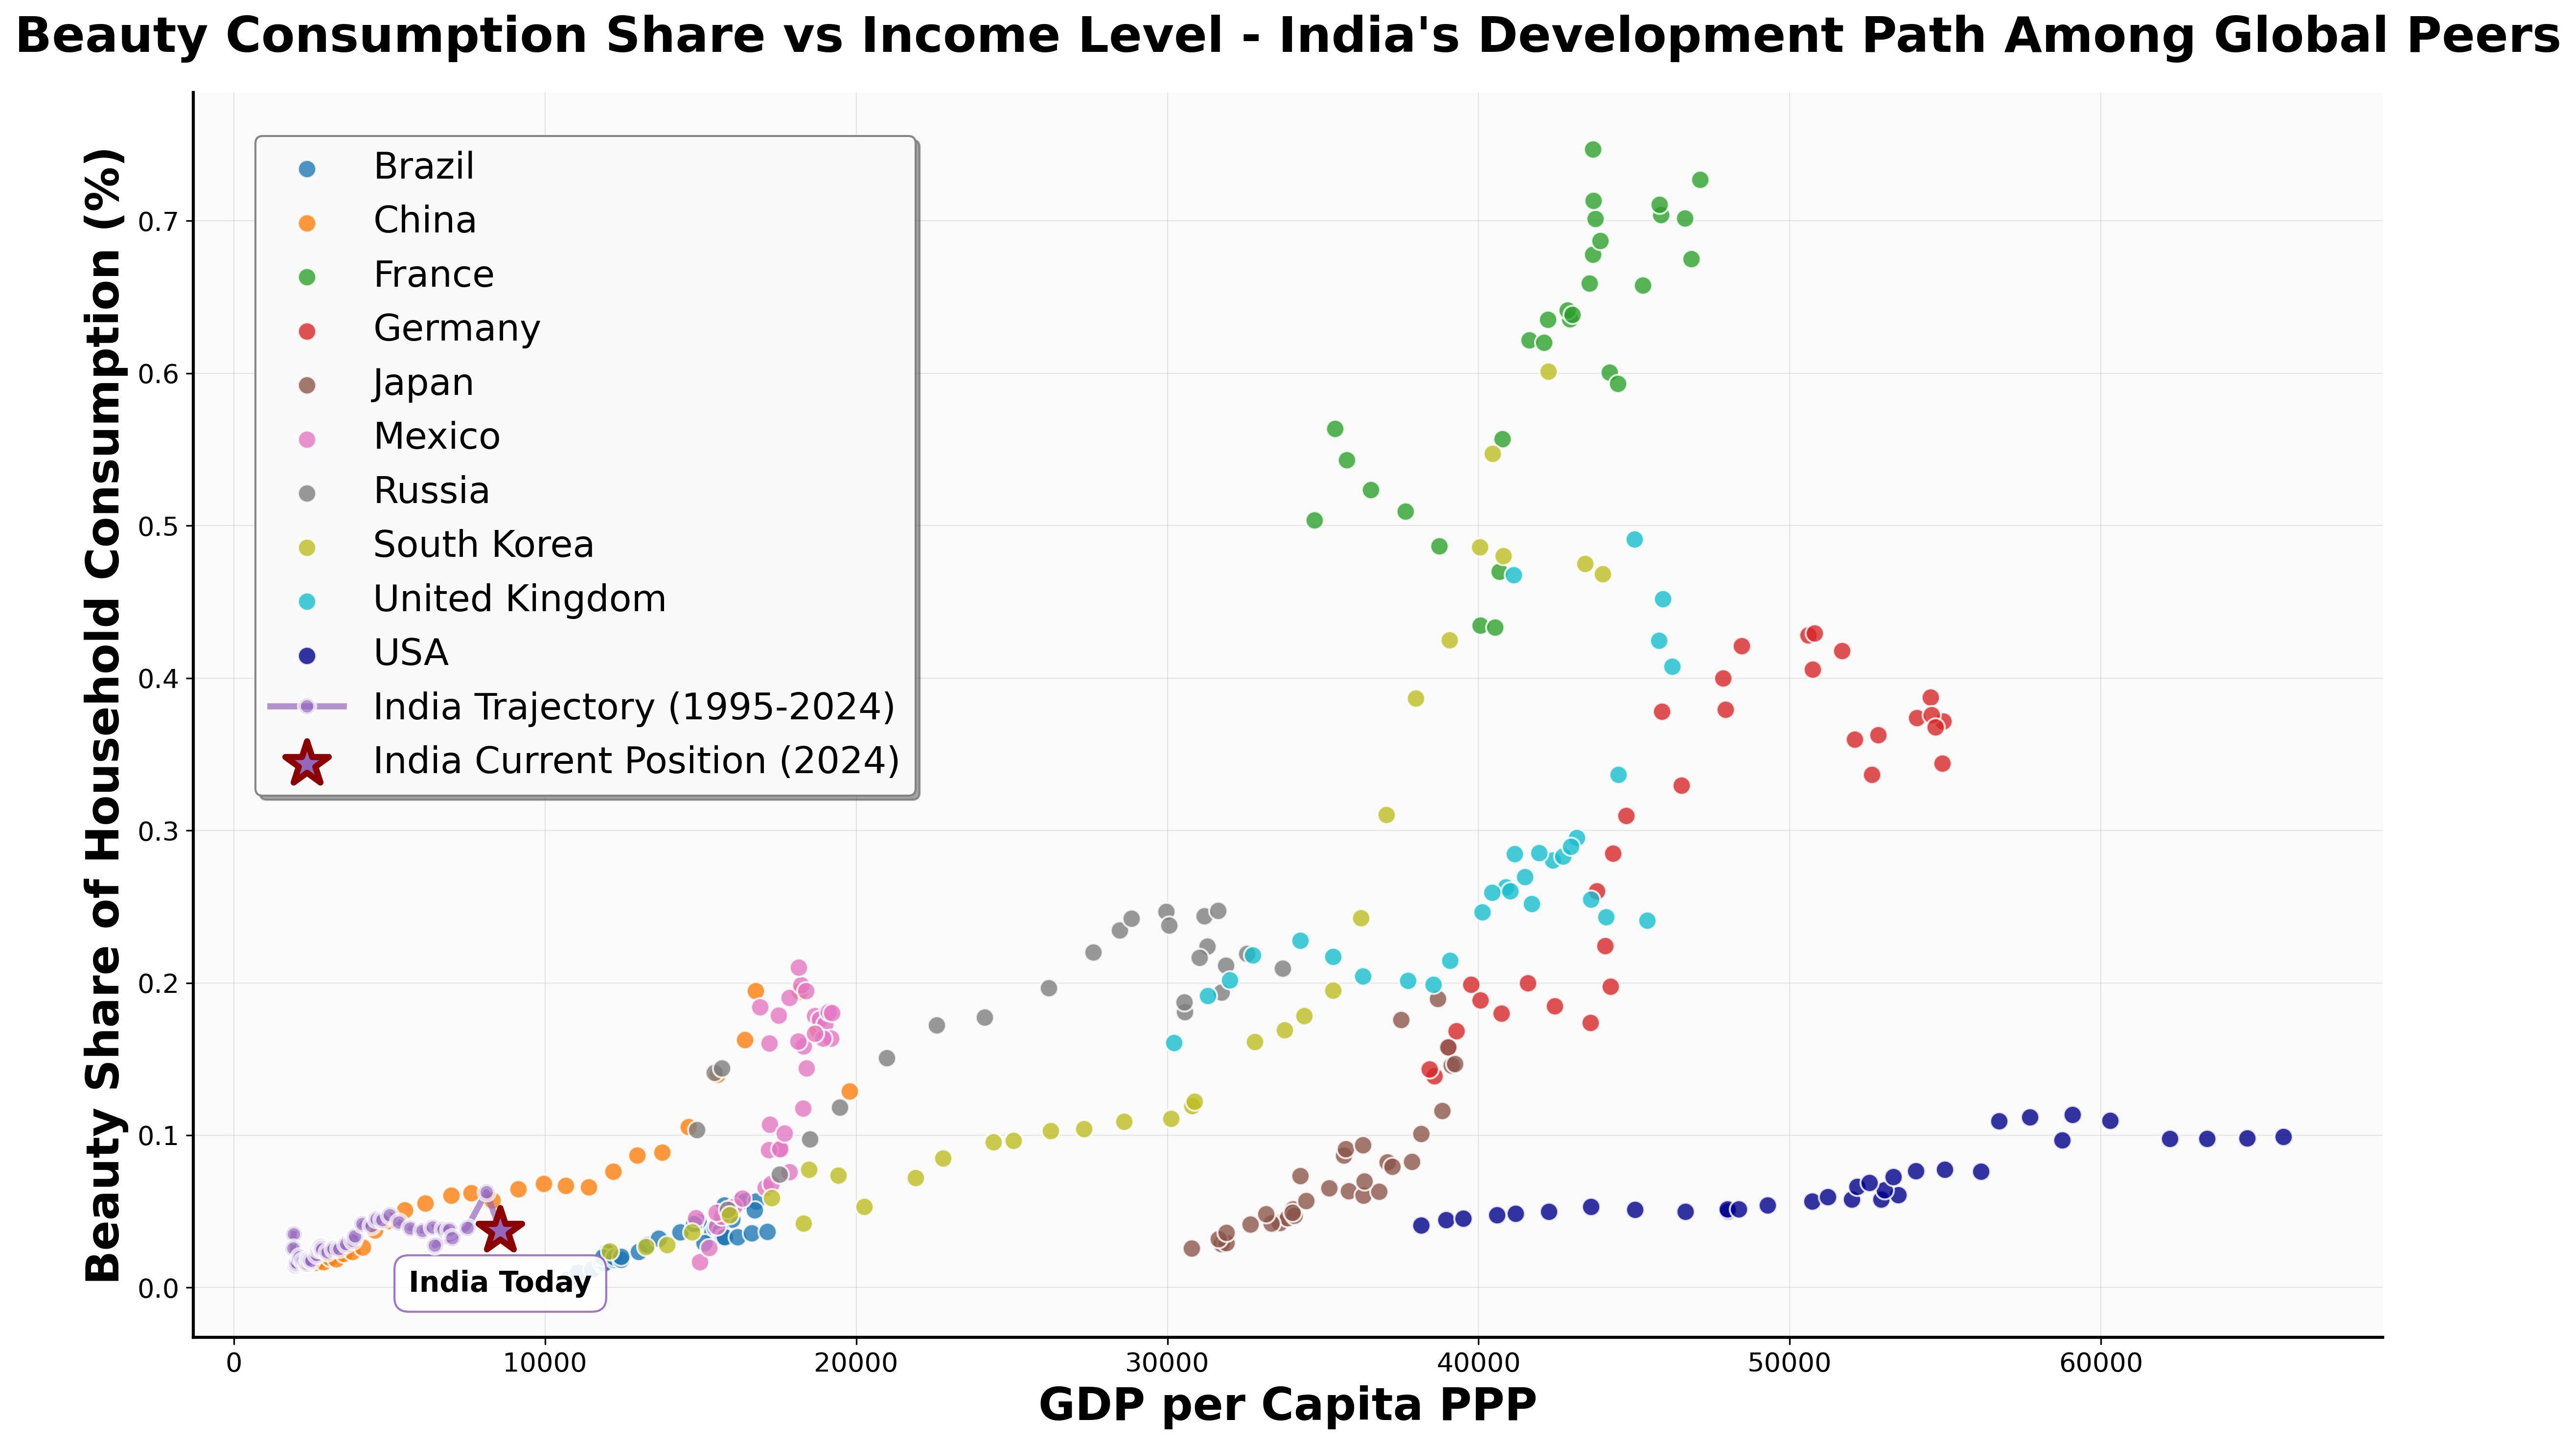
\includegraphics[width=1.1\textwidth]{T2-3_beauty_share_overlay.png}
    \caption{\textbf{India's Growth Trajectory}: Significant gap vs successful emerging market patterns}
\end{subfigure}
\hfill
\begin{subfigure}[b]{0.48\textwidth}
    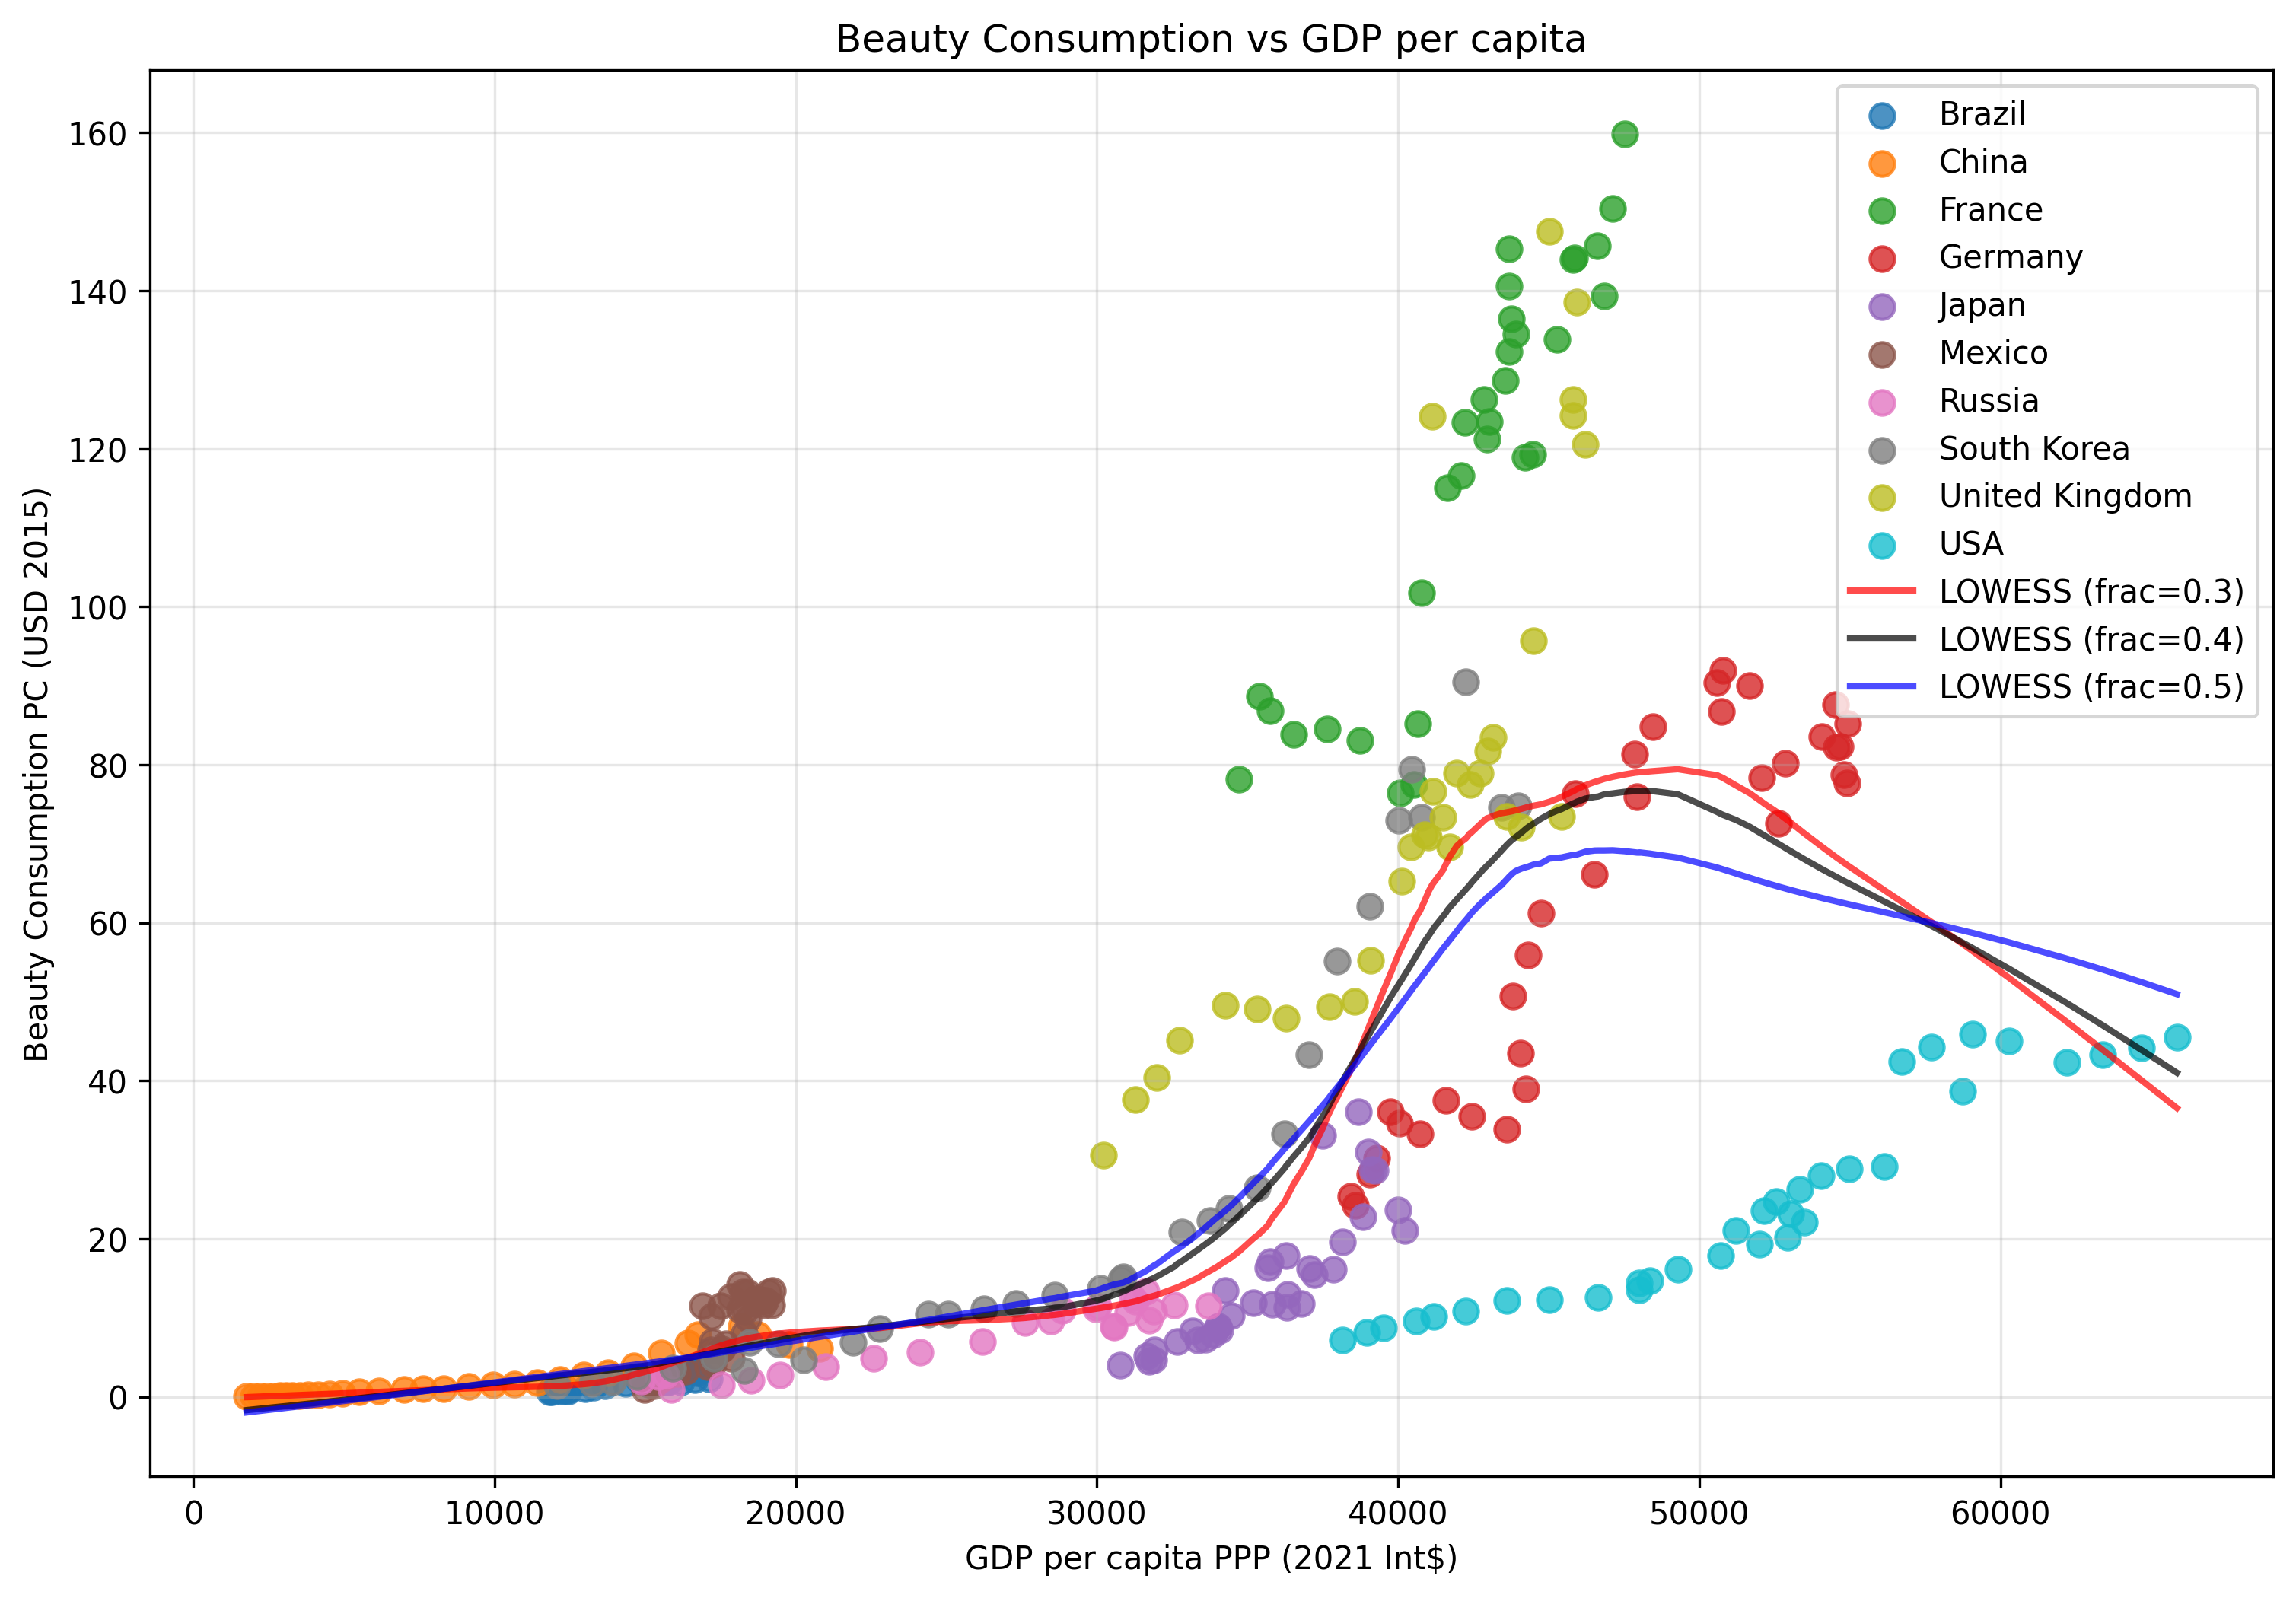
\includegraphics[width=\textwidth]{T1-3_BeautyPC_vs_gdppcppp_scatter.png}
    \caption{\textbf{Income-Beauty Relationship}: Raw data showing luxury good behavior across all countries}
\end{subfigure}
\caption{\textbf{Figure 1}: India's positioning and income-beauty relationship}
\end{figure}

\begin{figure}[H]
\centering
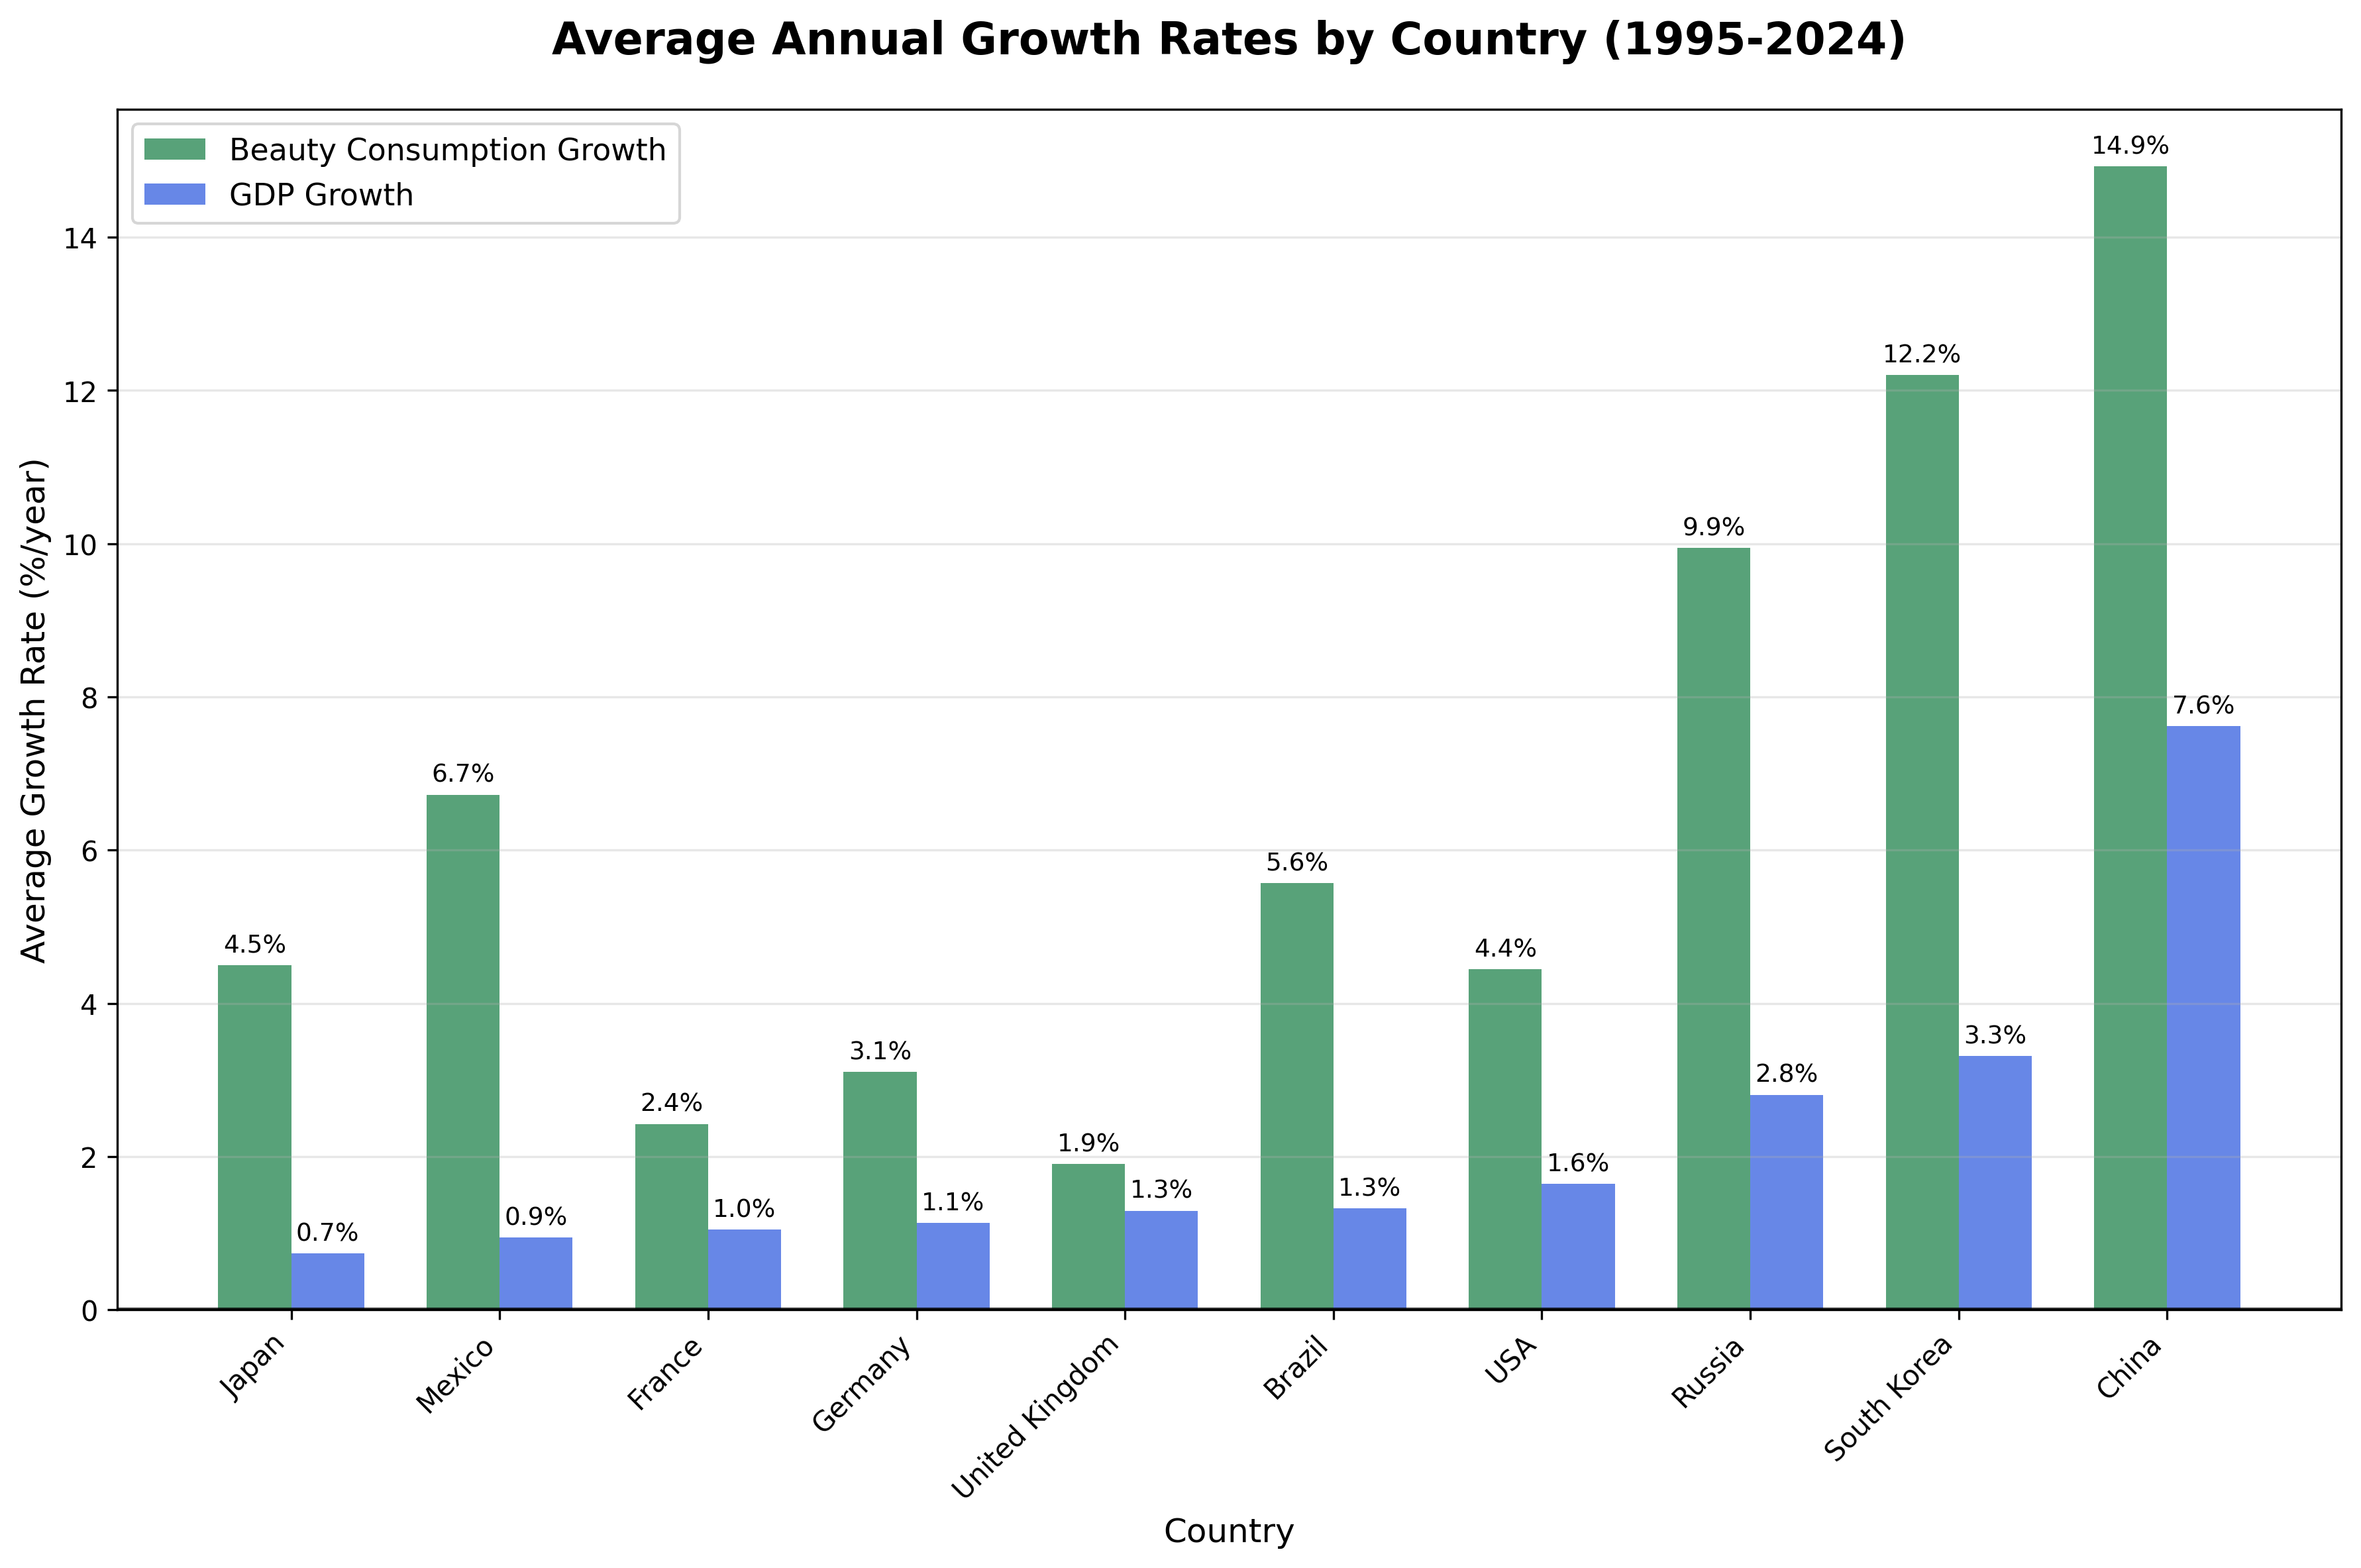
\includegraphics[width=0.7\textwidth]{T1-2_average_growth_rates_comparison.png}
\caption{\textbf{Figure 2}: Cross-country growth patterns by income level}
\end{figure}

\textbf{Investment Implications:} India presents \textbf{compelling opportunity with significant upside potential}. The \textbf{substantial performance gap versus peers} indicates room for dramatic growth. South Korea's precedent shows \textbf{acceleration can occur through catalysts} before reaching traditional thresholds. \textbf{Priority areas}: skincare and women's beauty segments show \textbf{strongest threshold growth patterns}.

% Task 1: Statistical Exploration
\section{Task 1: Statistical Exploration}

\textbf{What We Did:} We analyzed beauty spending vs income relationships across 10 countries using correlation analysis, income elasticity measurement, and piecewise regression to identify structural breaks where consumption patterns fundamentally change.

\textbf{What the Numbers Show:}
\vspace{-3pt}
\begin{itemize}
    \setlength{\itemsep}{1pt}
    \item Beauty exhibits \textbf{luxury good behavior with 2.3x income elasticity}—spending increases 2.3\% for every 1\% income increase
    \item Remarkably strong relationship (R² > 0.8) with \textbf{structural breaks around \$40-50k GDP per capita}
    \item Before threshold: moderate elasticity; after crossing: relationship strengthens significantly, confirming disproportionate acceleration
\end{itemize}

\begin{figure}[H]
\centering
\begin{subfigure}[b]{0.48\textwidth}
    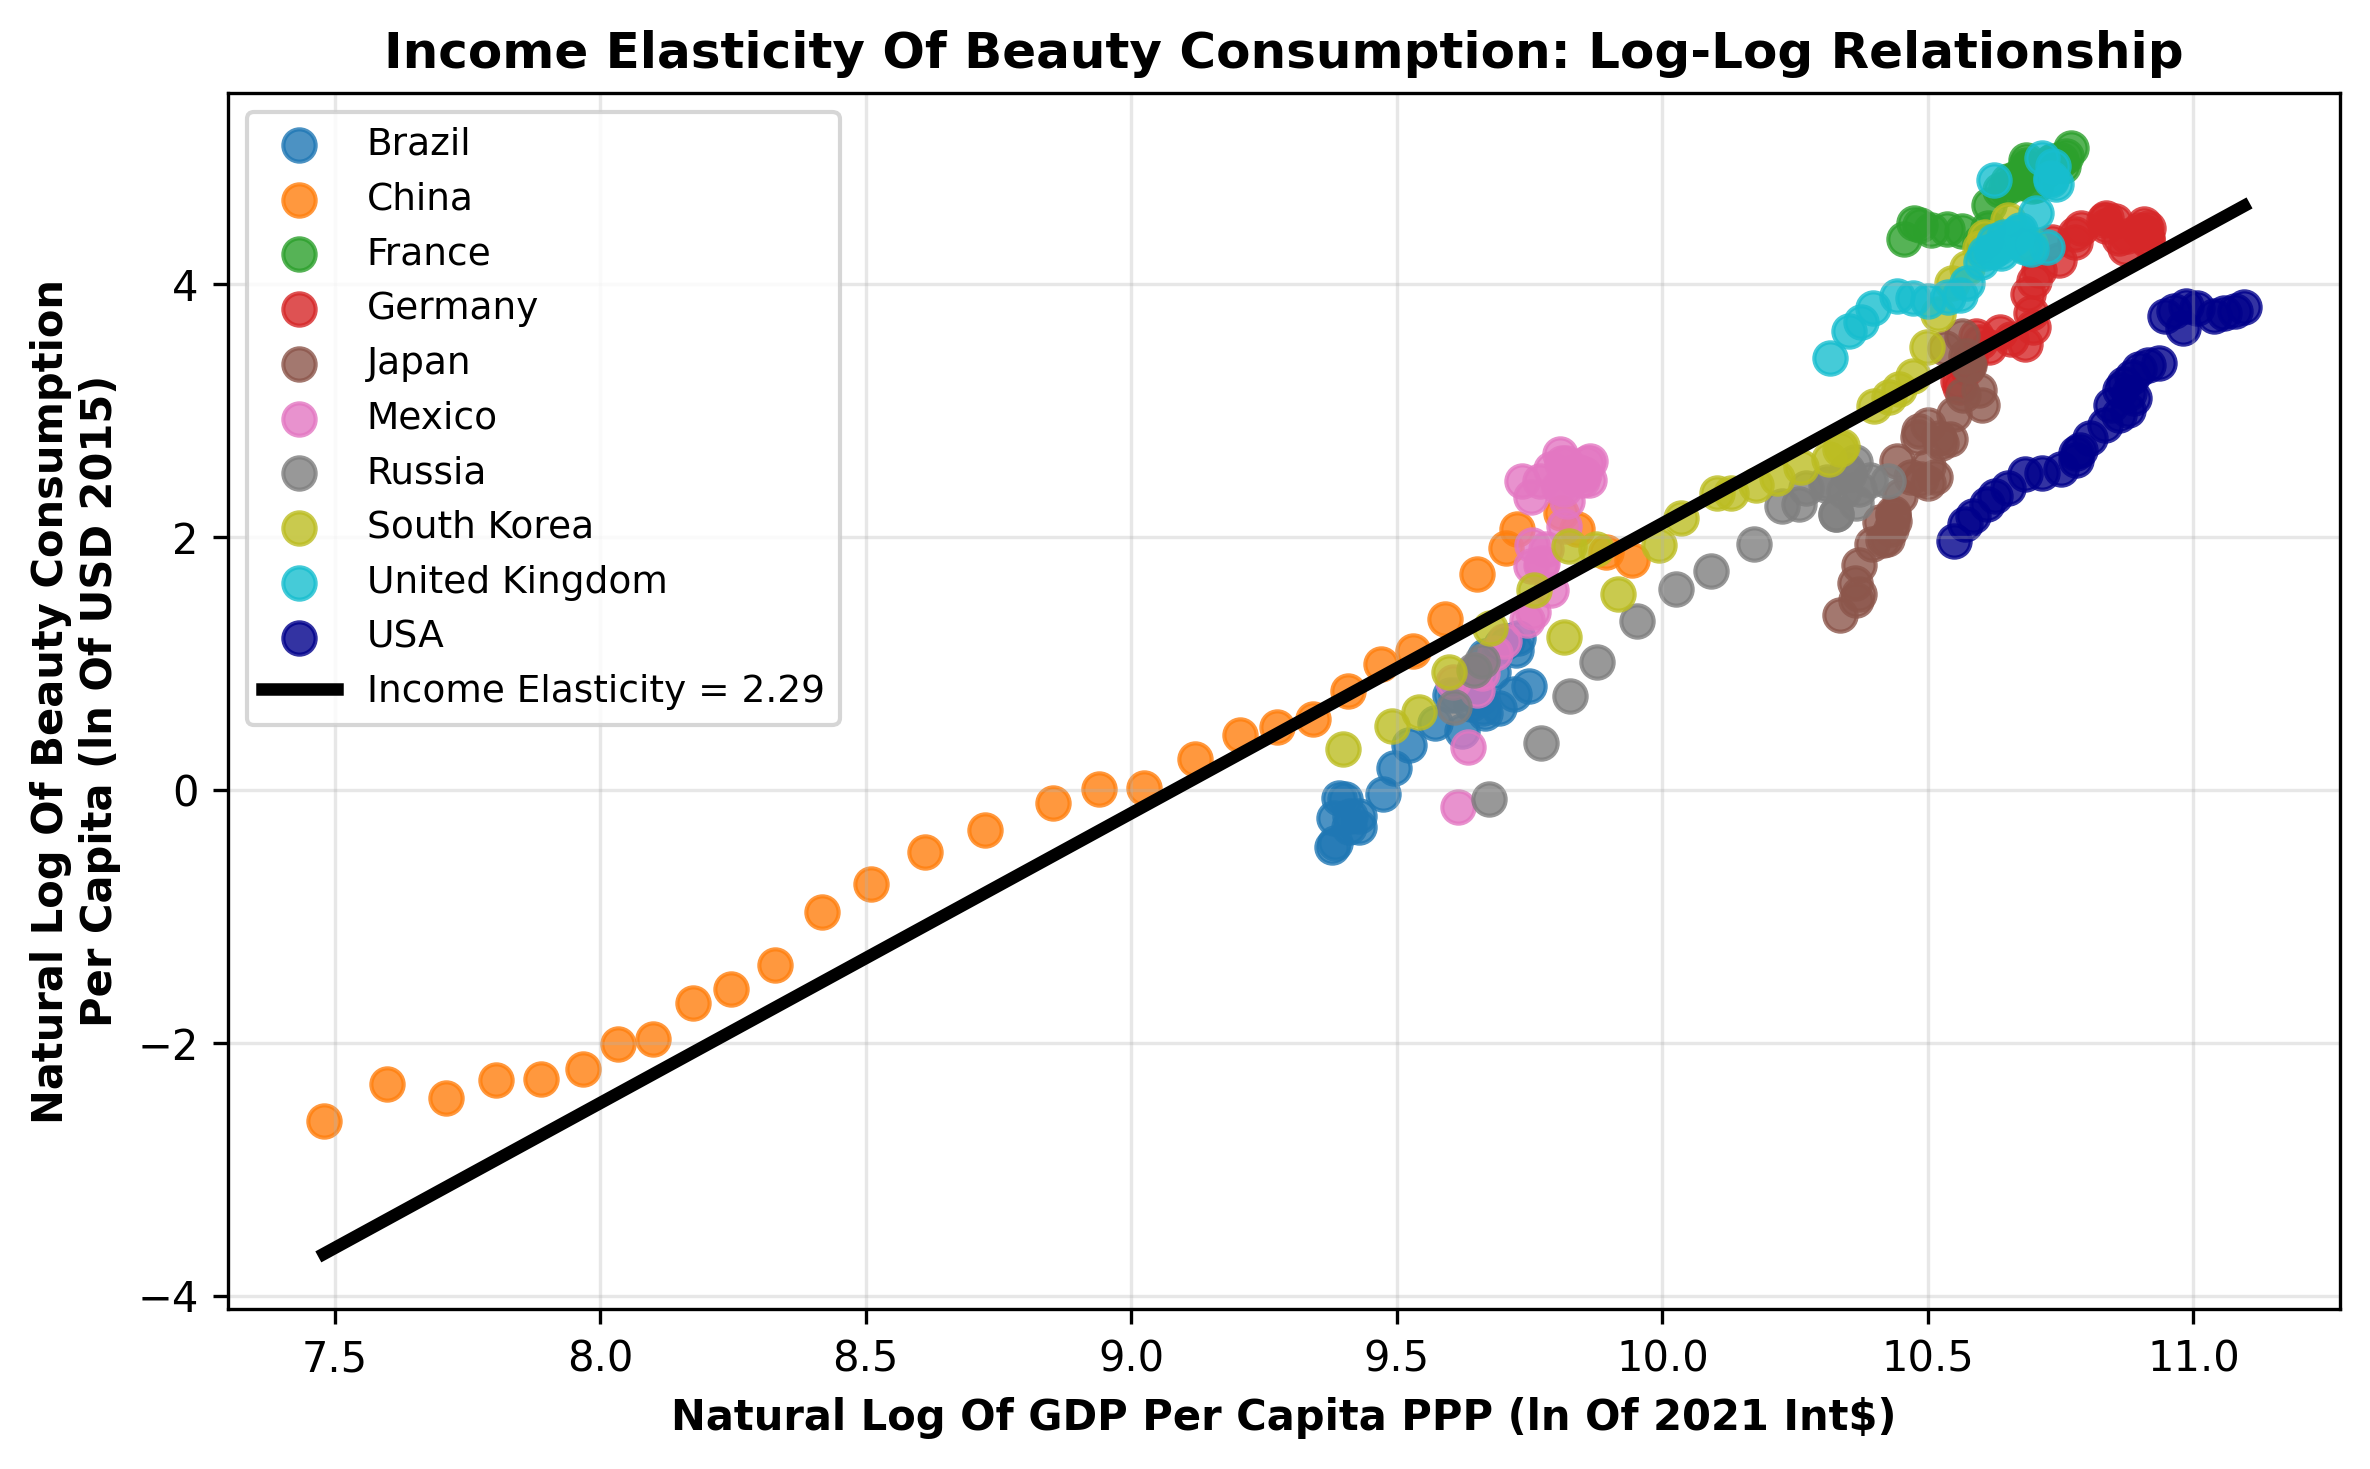
\includegraphics[width=\textwidth]{T1-4_log_scatter_ols.png}
    \caption{\textbf{Income Elasticity}: 2.3x coefficient confirms luxury classification}
\end{subfigure}
\hfill
\begin{subfigure}[b]{0.48\textwidth}
    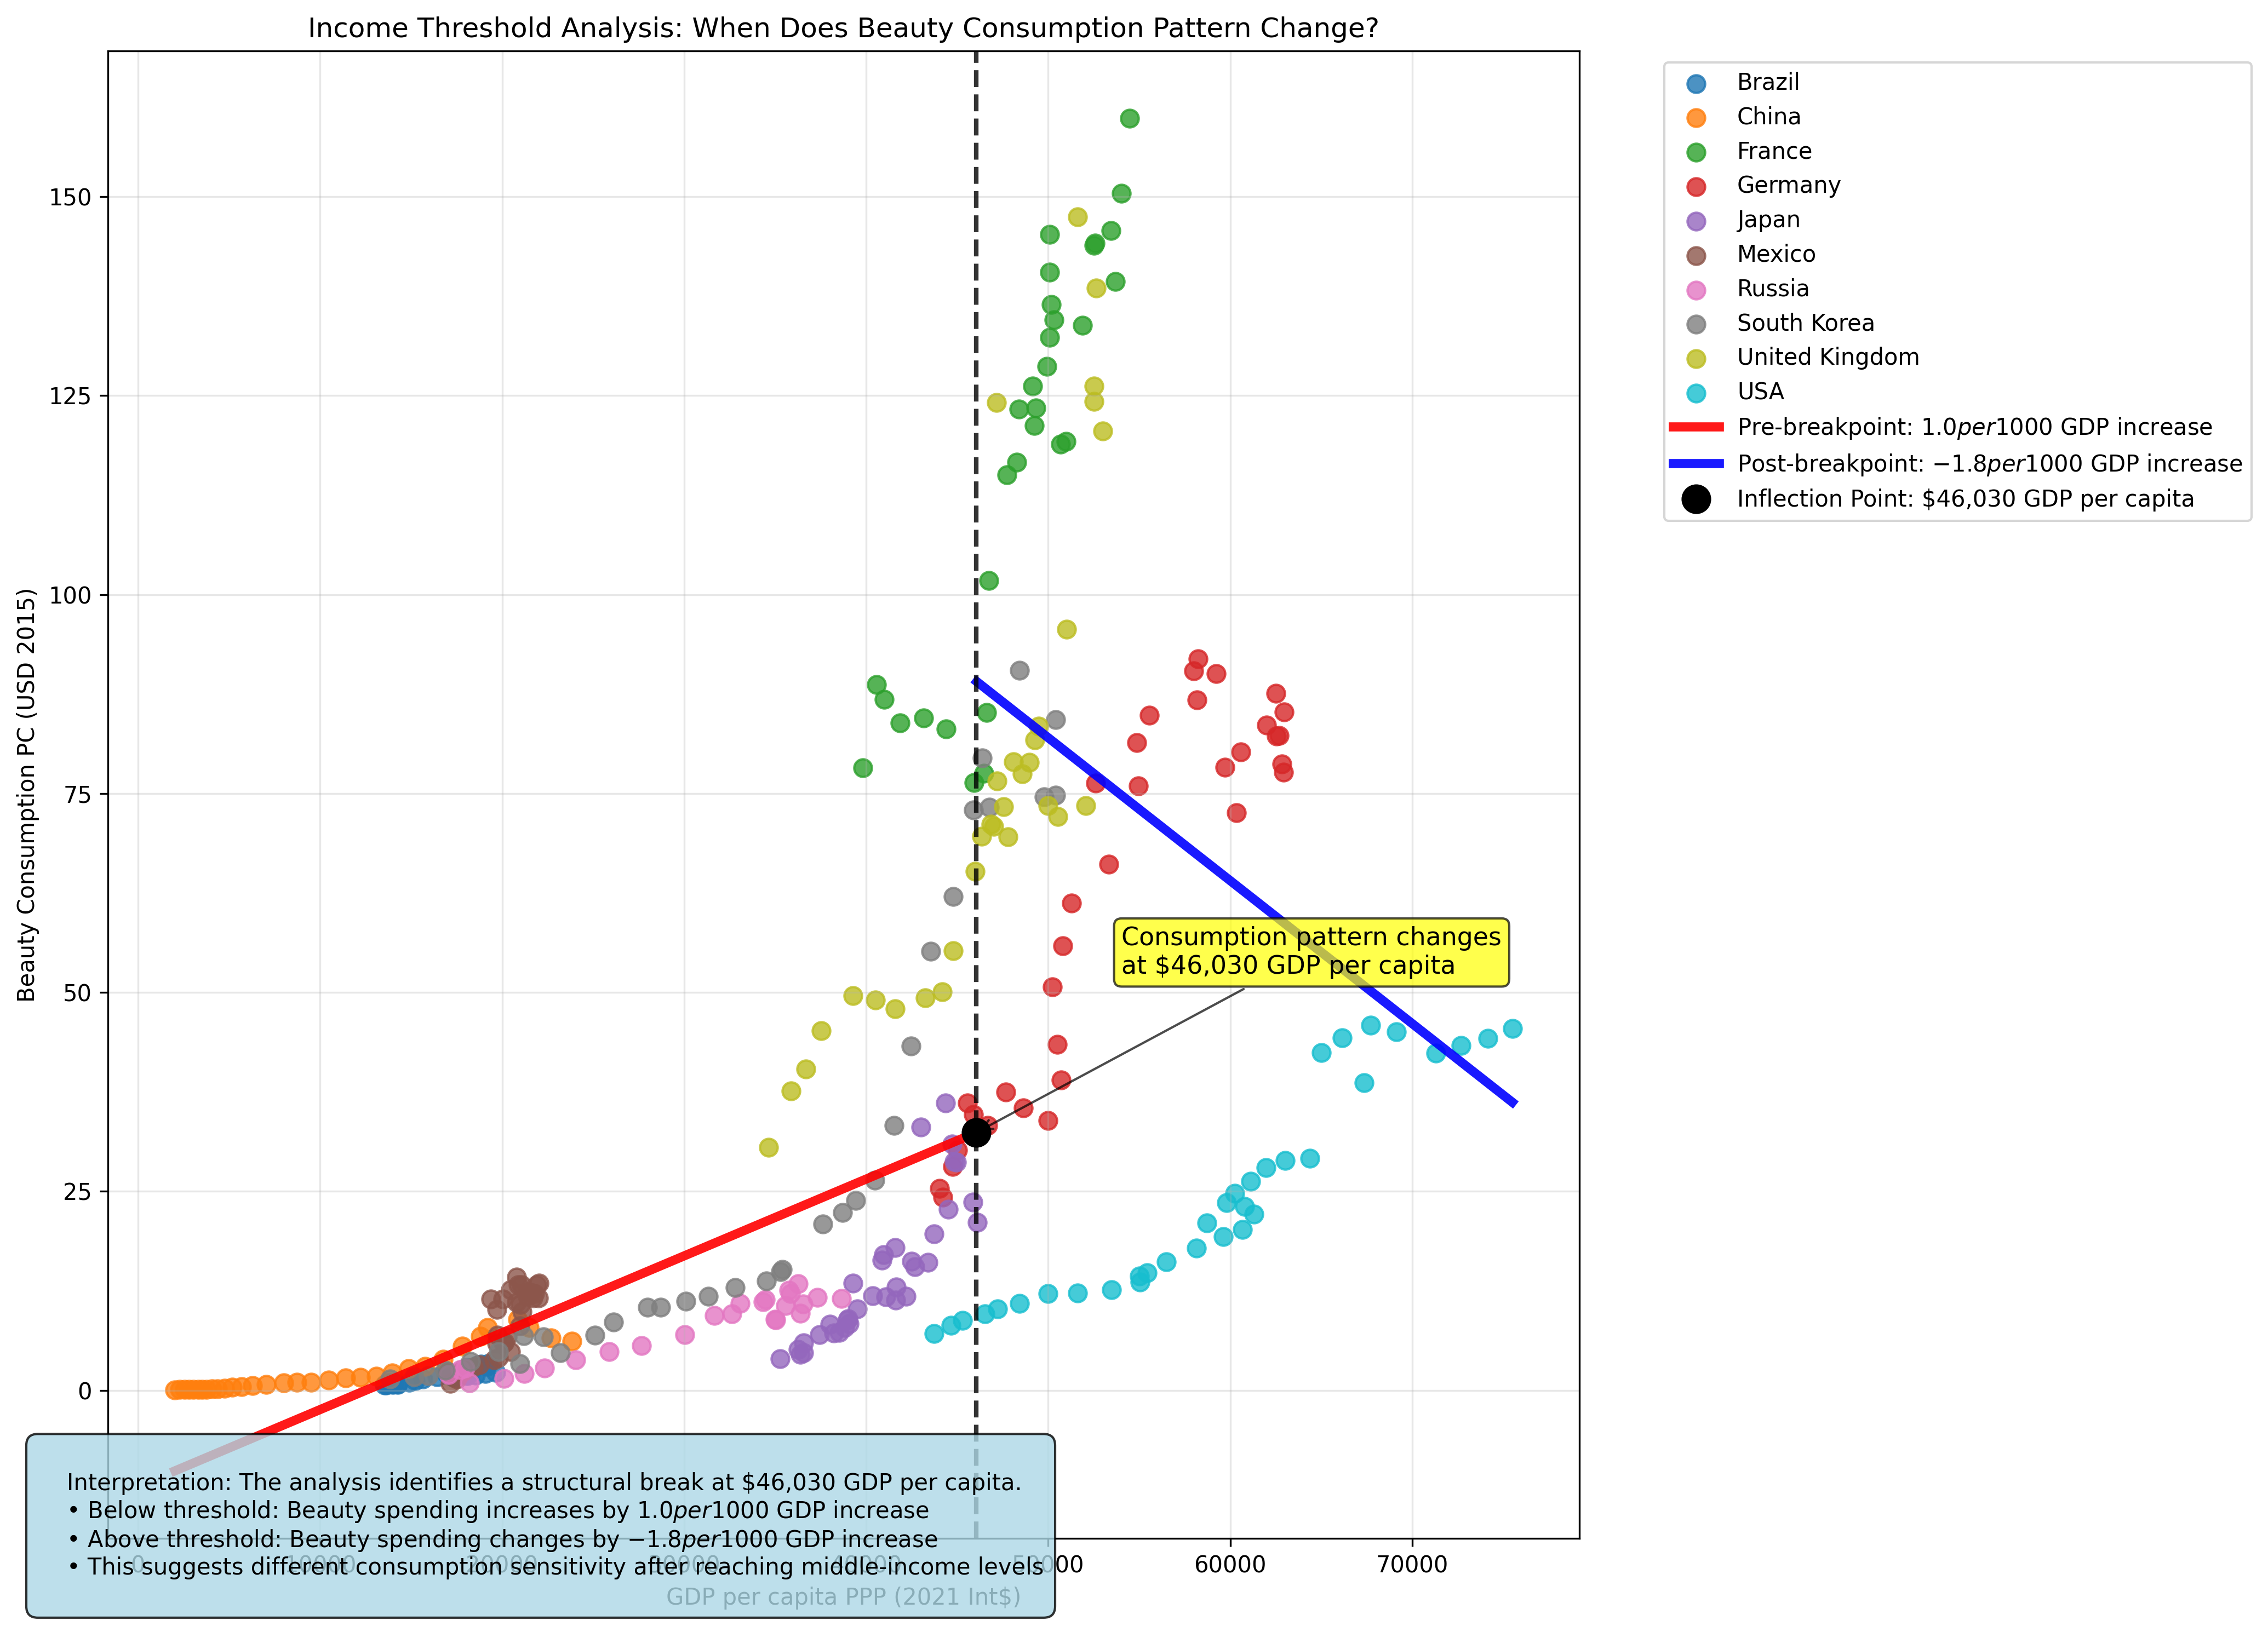
\includegraphics[width=\textwidth]{T1-6_piecewise_regression.png}
    \caption{\textbf{Structural Breaks}: Clear inflection points validate thresholds}
\end{subfigure}
\caption{\textbf{Figure 3}: Statistical Foundation - Income elasticity evidence and structural break analysis demonstrating luxury good behavior}
\end{figure}

\begin{figure}[H]
\centering
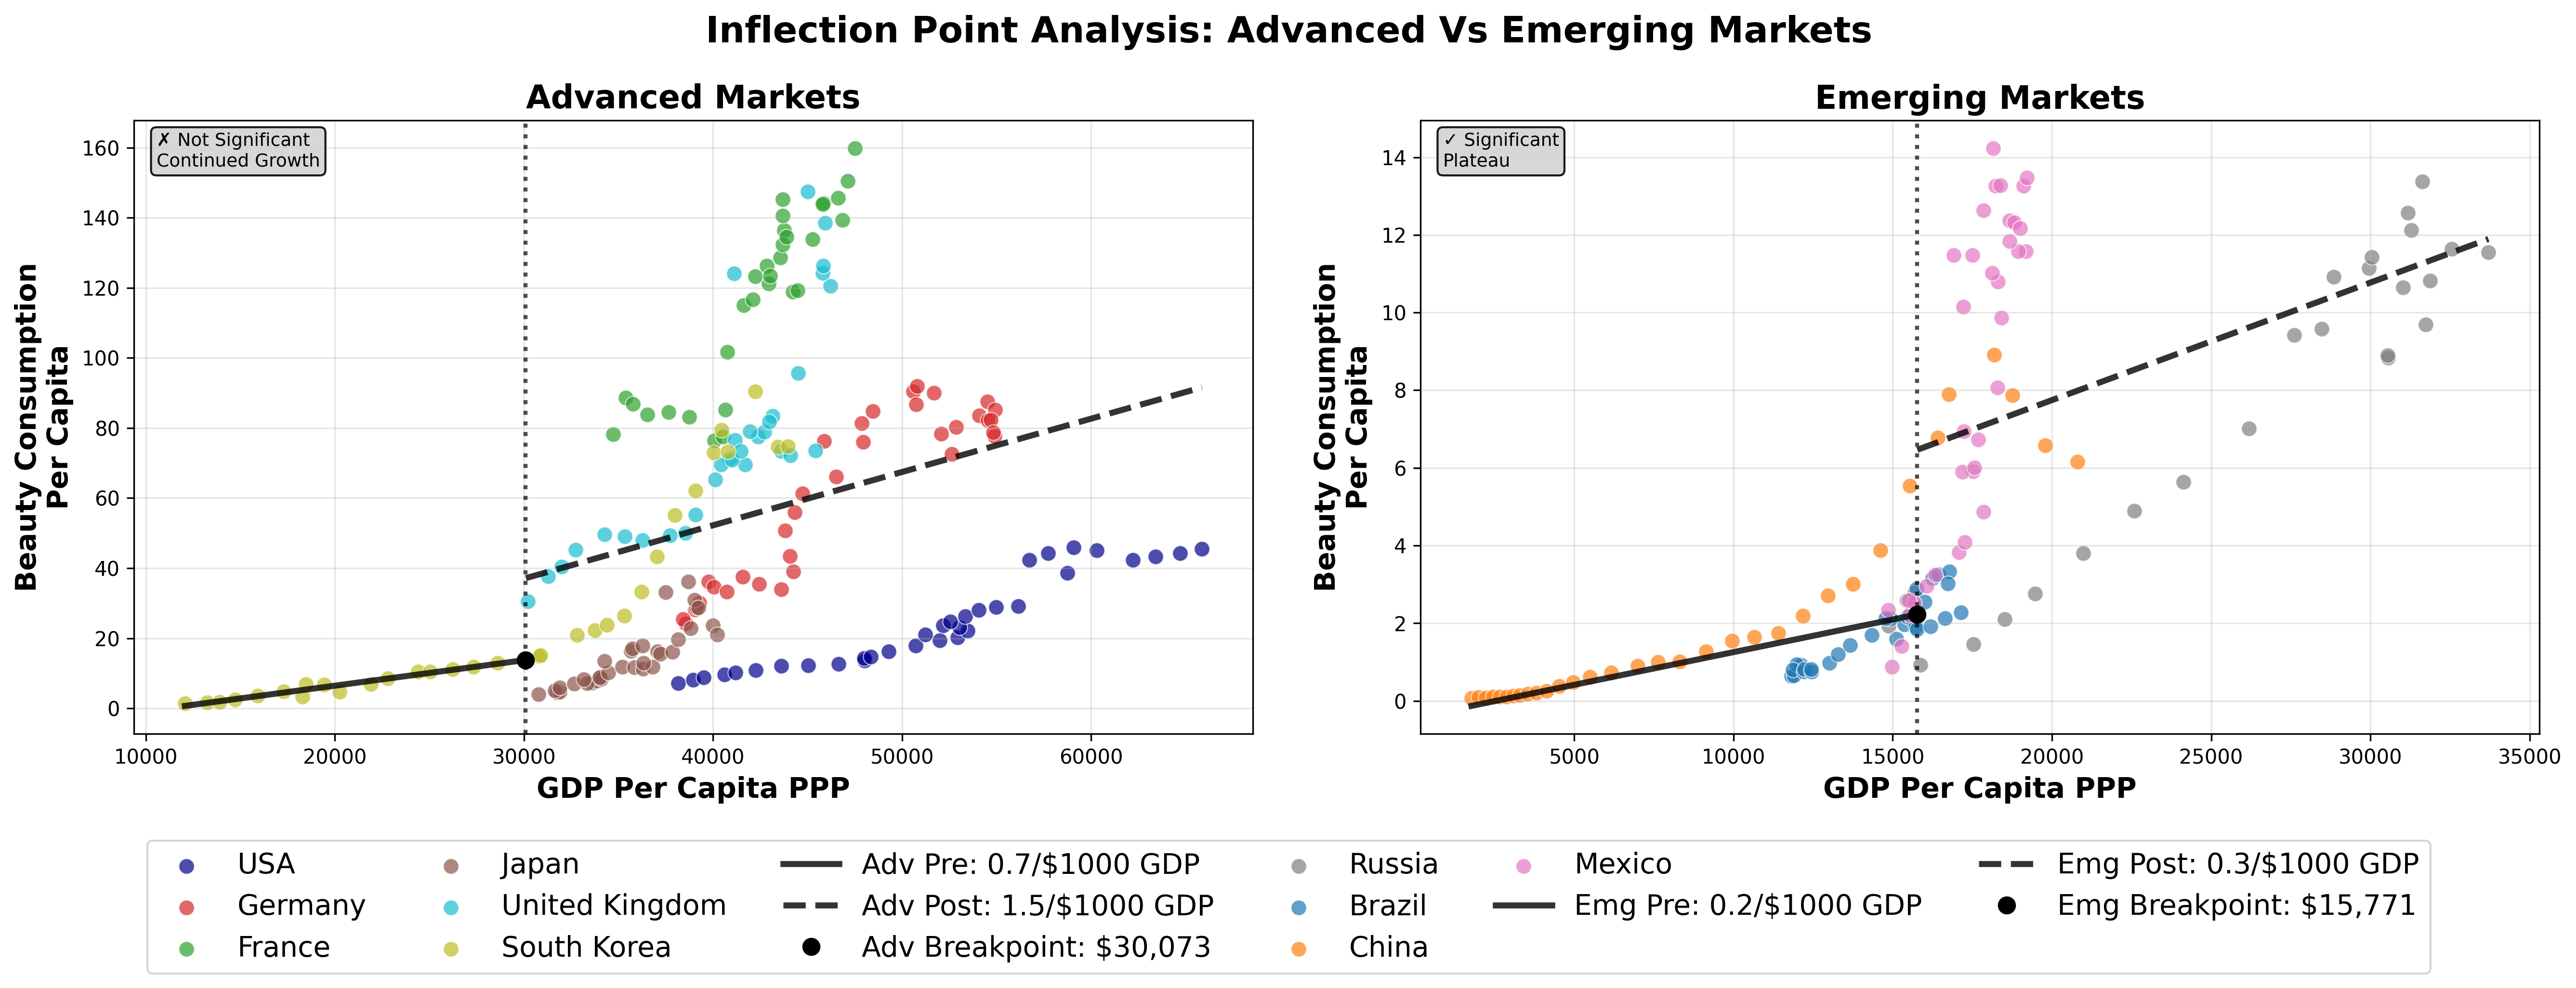
\includegraphics[width=1.0\textwidth]{T1-7_segmented_inflection_comparison.png}
\caption{\textbf{Figure 4}: Country-Specific Threshold Analysis - Country-by-country breakdown of identified threshold points, showing heterogeneity in breakpoint timing and magnitude across different markets}
\end{figure}

\begin{figure}[H]
\centering
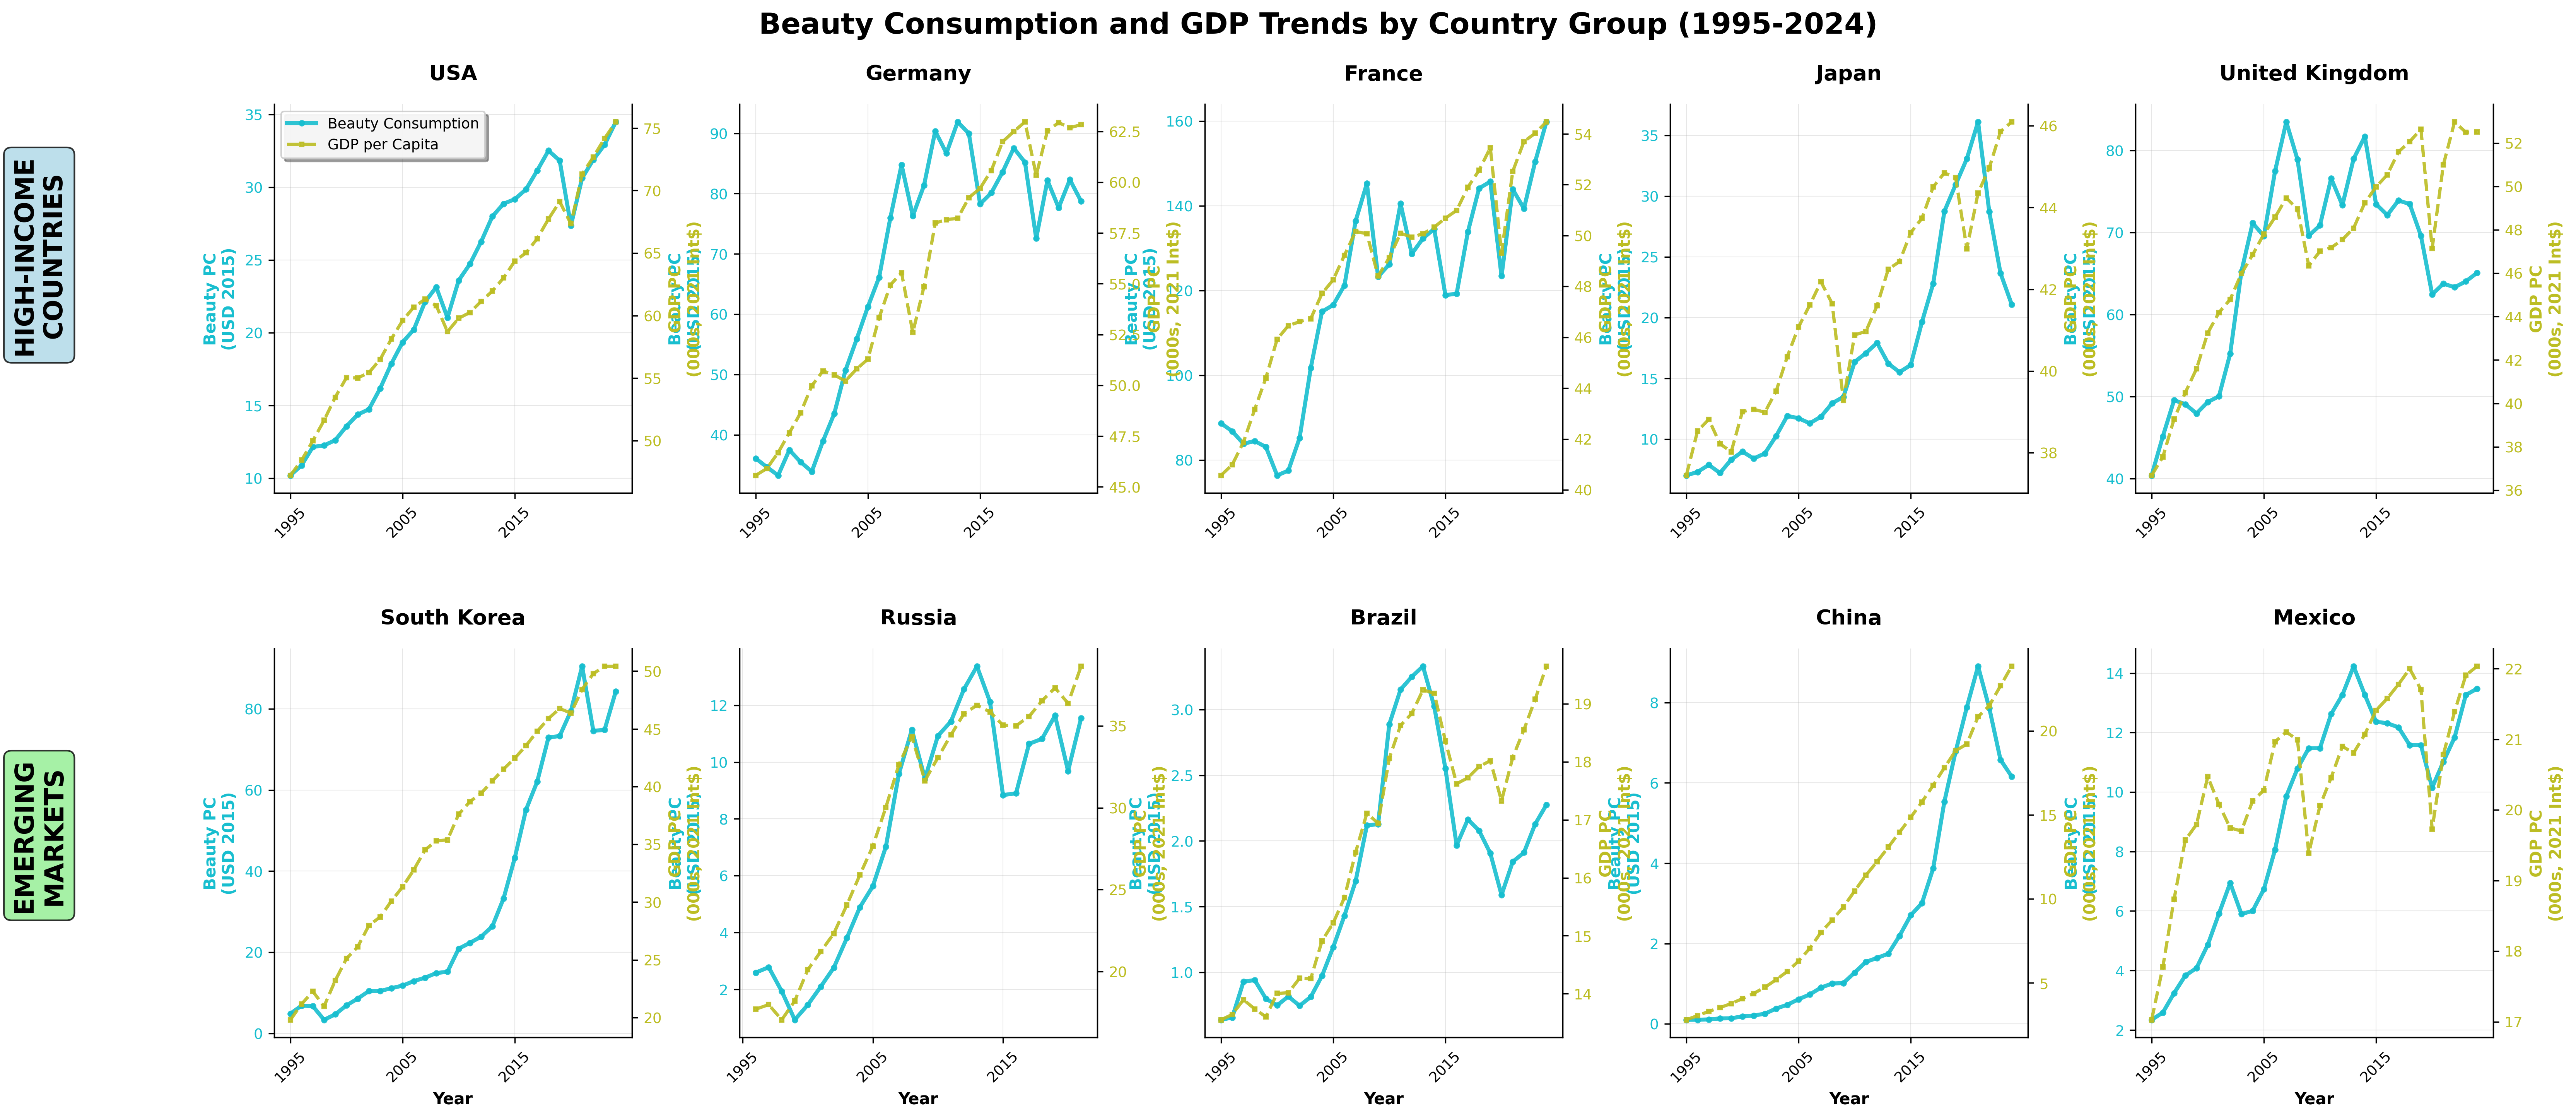
\includegraphics[width=1.0\textwidth]{T1-1_small_multiples_by_income_group.png}
\caption{\textbf{Figure 5}: Income Group Analysis - Consumption patterns segmented by income levels, demonstrating clear progression in beauty spending as countries develop economically}
\end{figure}

\textbf{Key Takeaways:}
\vspace{-3pt}
\begin{itemize}
    \setlength{\itemsep}{1pt}
    \item 2.3x elasticity means beauty markets grow \textbf{more than twice as fast as the economy}, attractive for growth investors
    \item Consistent \$40-50k thresholds provide \textbf{clear market entry timing frameworks}
    \item Strong explanatory power (R² > 0.8) reduces forecasting uncertainty through predictable relationships
    \item Income group segmentation shows \textbf{distinct consumption phases} guiding targeted investment strategies
\end{itemize}
\textit{See Appendix Section B for additional statistical evidence.}

% Task 2: Comparative Benchmarking
\section{Task 2: Comparative Benchmarking}

\textbf{What We Did:} We performed income-matched peer analysis, identifying when other countries had similar GDP levels to India today (\$8,563), then calculated 5-year post-match CAGR to understand expected growth trajectories. We also conducted clustering analysis to assess India's position relative to different growth patterns.

\textbf{What the Numbers Show:}
\vspace{-3pt}
\begin{itemize}
    \setlength{\itemsep}{1pt}
    \item \textbf{India significantly underperforms peers} with 5-year CAGR of \textbf{4.1\%} vs Brazil (32.8\%), South Korea (28.6\%), China (16.6\%), Mexico (21.7\%)
    \item Growth trajectory stable but not accelerating (p=0.695), suggesting India hasn't entered rapid consumption phase
    \item Clustering analysis places India in \textbf{stable, lower-growth segment} with persistent rather than transitional patterns
\end{itemize}

\begin{figure}[H]
\centering
\begin{subfigure}[b]{0.48\textwidth}
    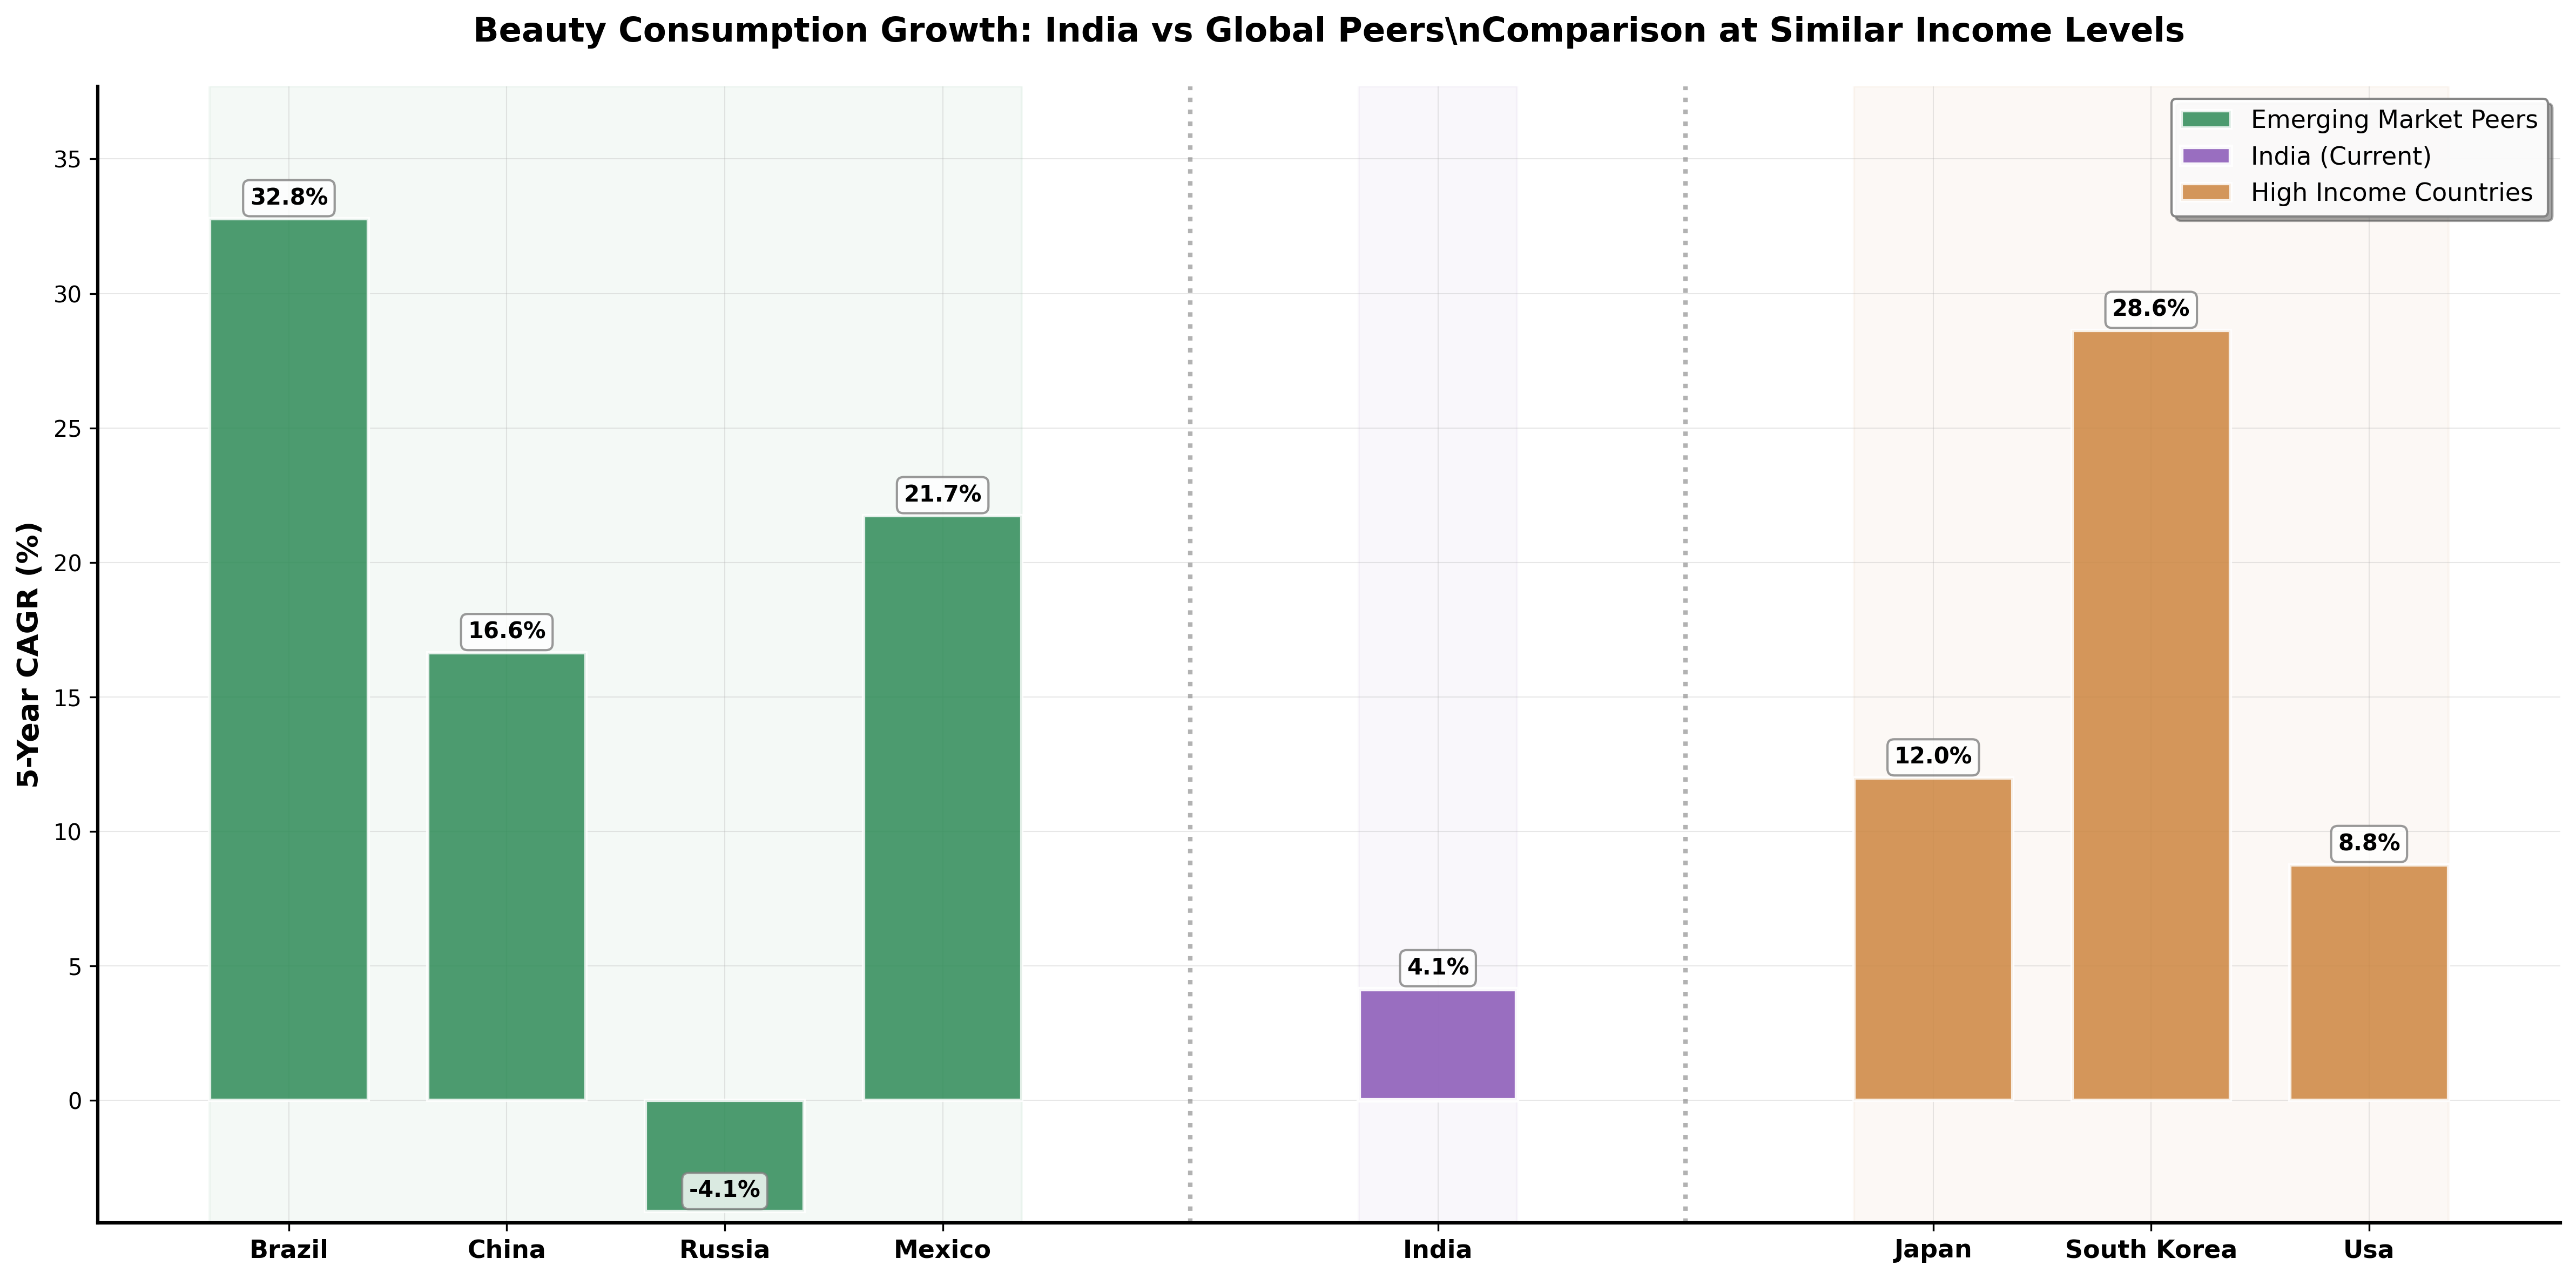
\includegraphics[width=\textwidth]{T2-1_cagr_comparison.png}
    \caption{\textbf{Growth Gap}: India's 4.1\% vs peer performance}
\end{subfigure}
\hfill
\begin{subfigure}[b]{0.48\textwidth}
    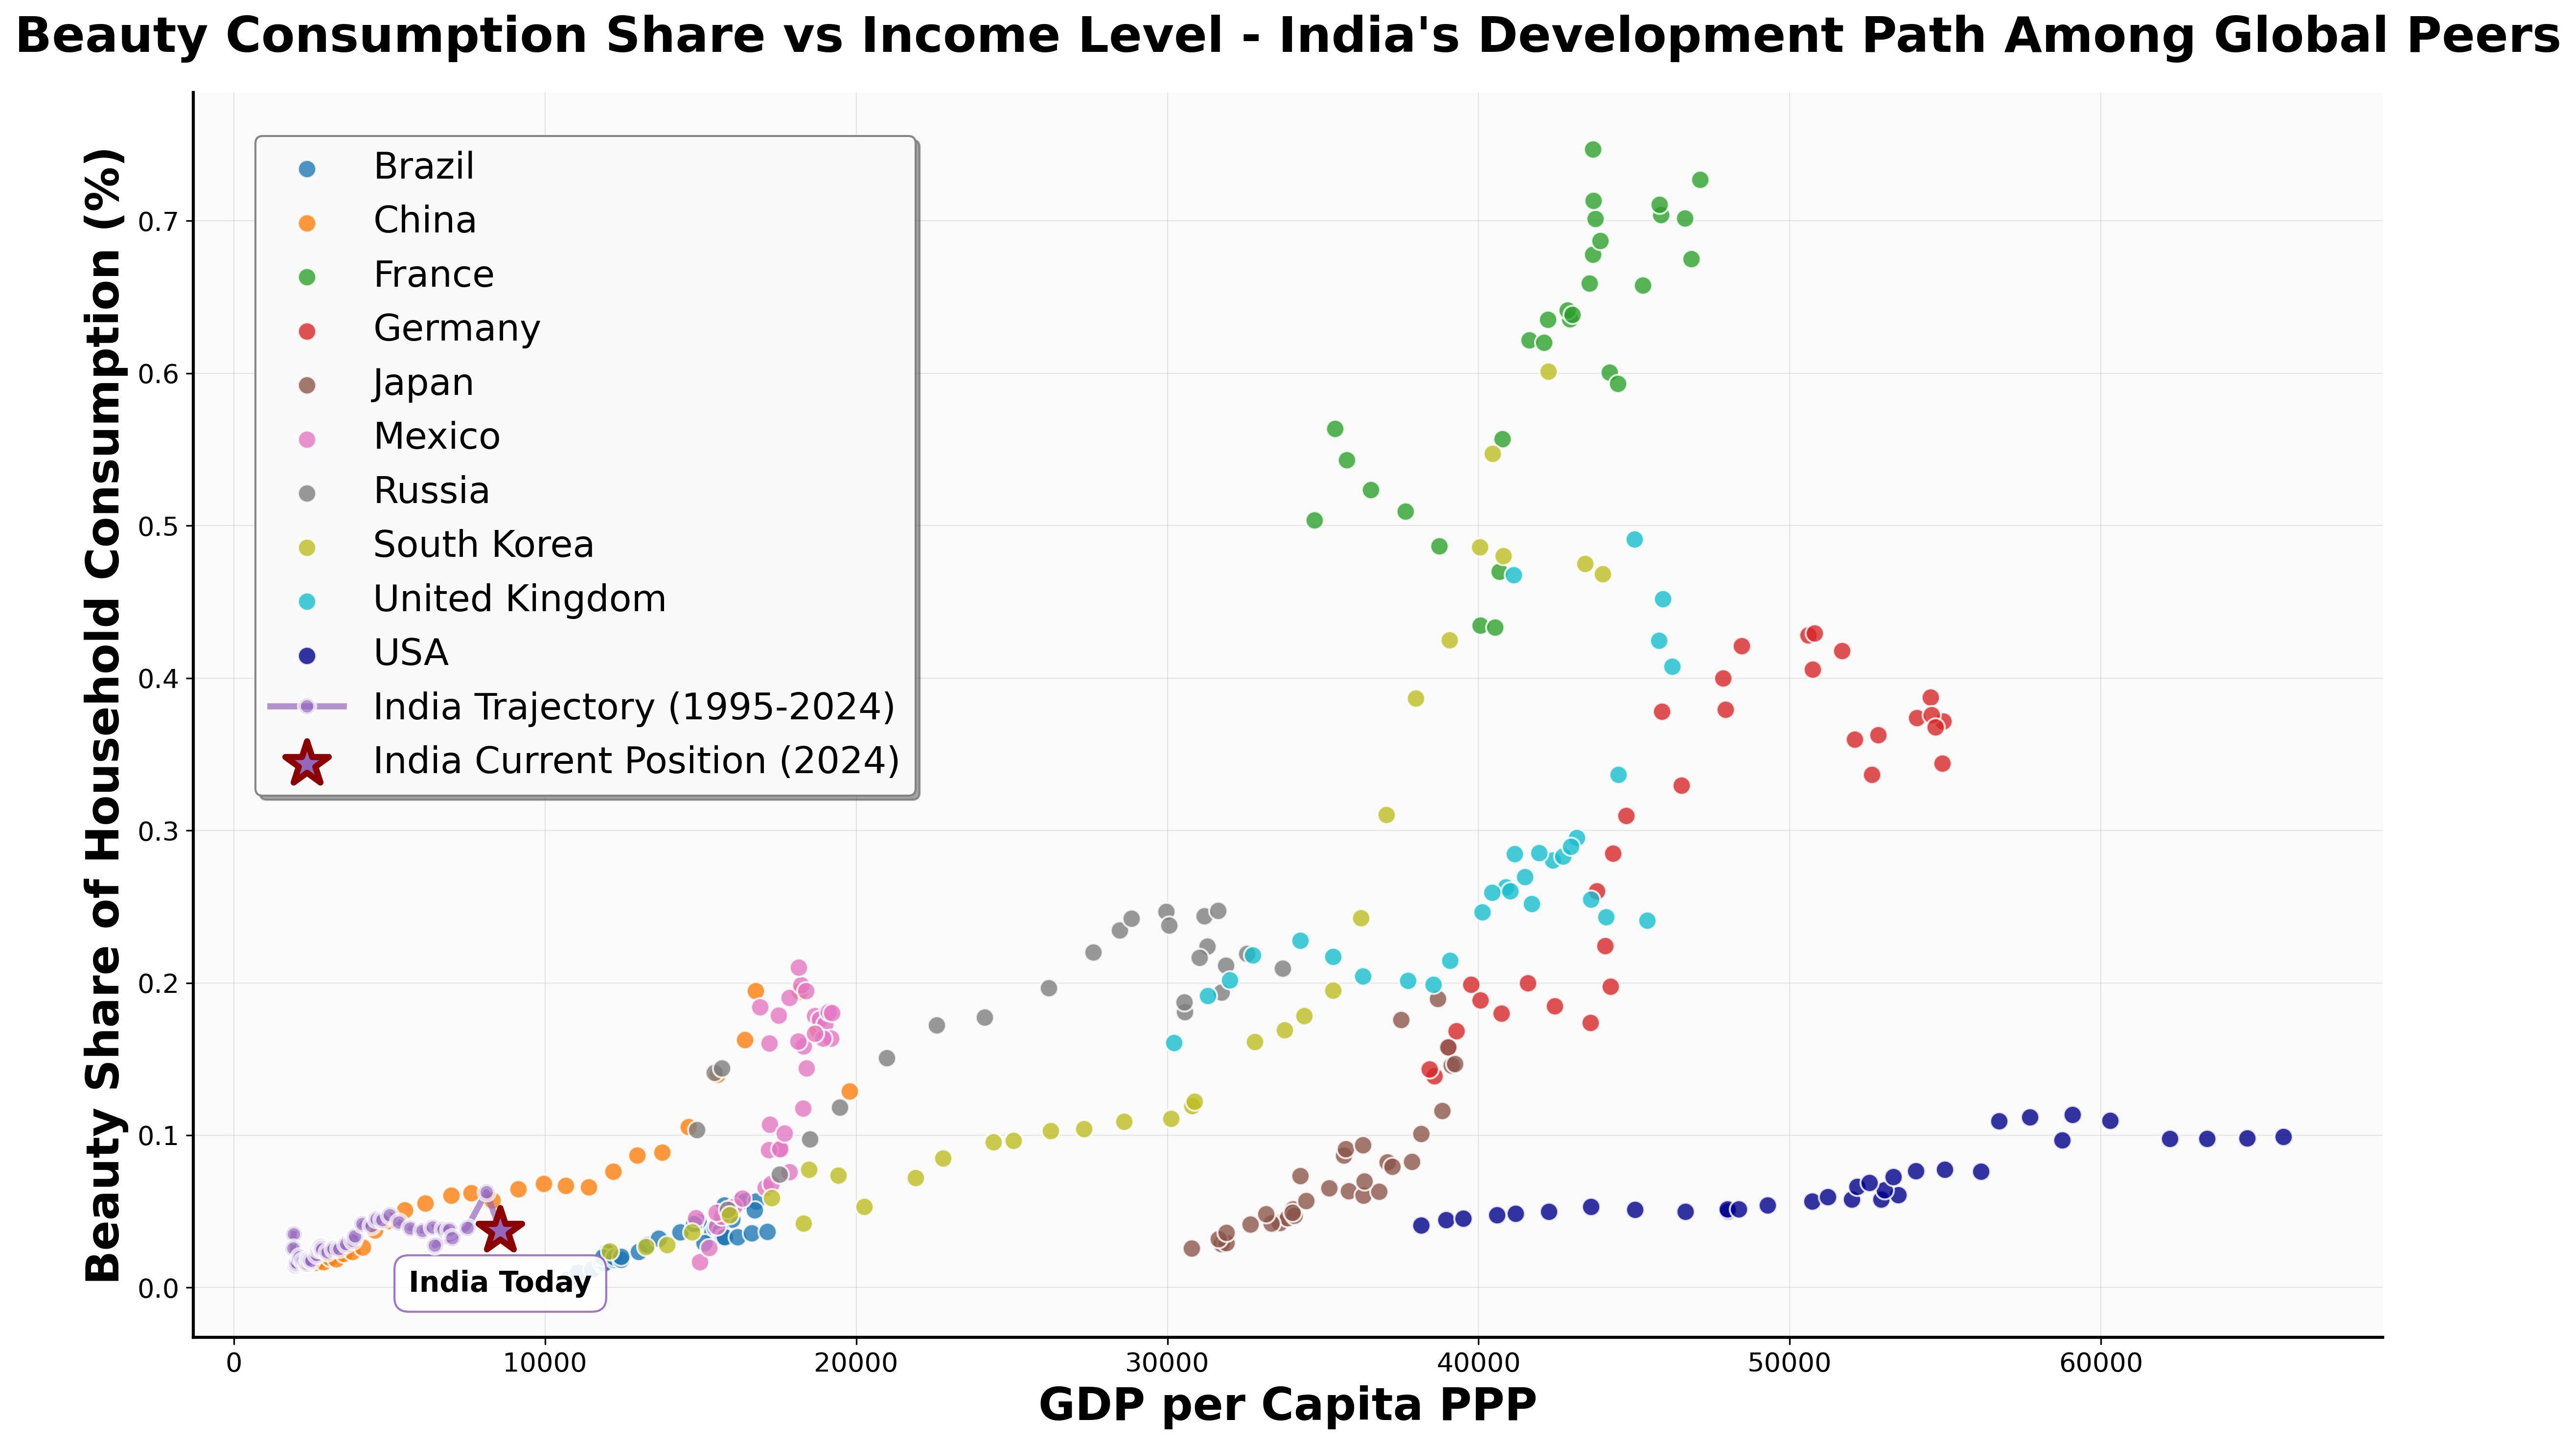
\includegraphics[width=\textwidth]{T2-3_beauty_share_overlay.png}
    \caption{\textbf{Share Evolution}: India vs successful emerging patterns}
\end{subfigure}
\caption{\textbf{Figure 6}: India's Underperformance - Comparative analysis showing significant growth gap versus income-matched peers}
\end{figure}

\begin{figure}[H]
\centering
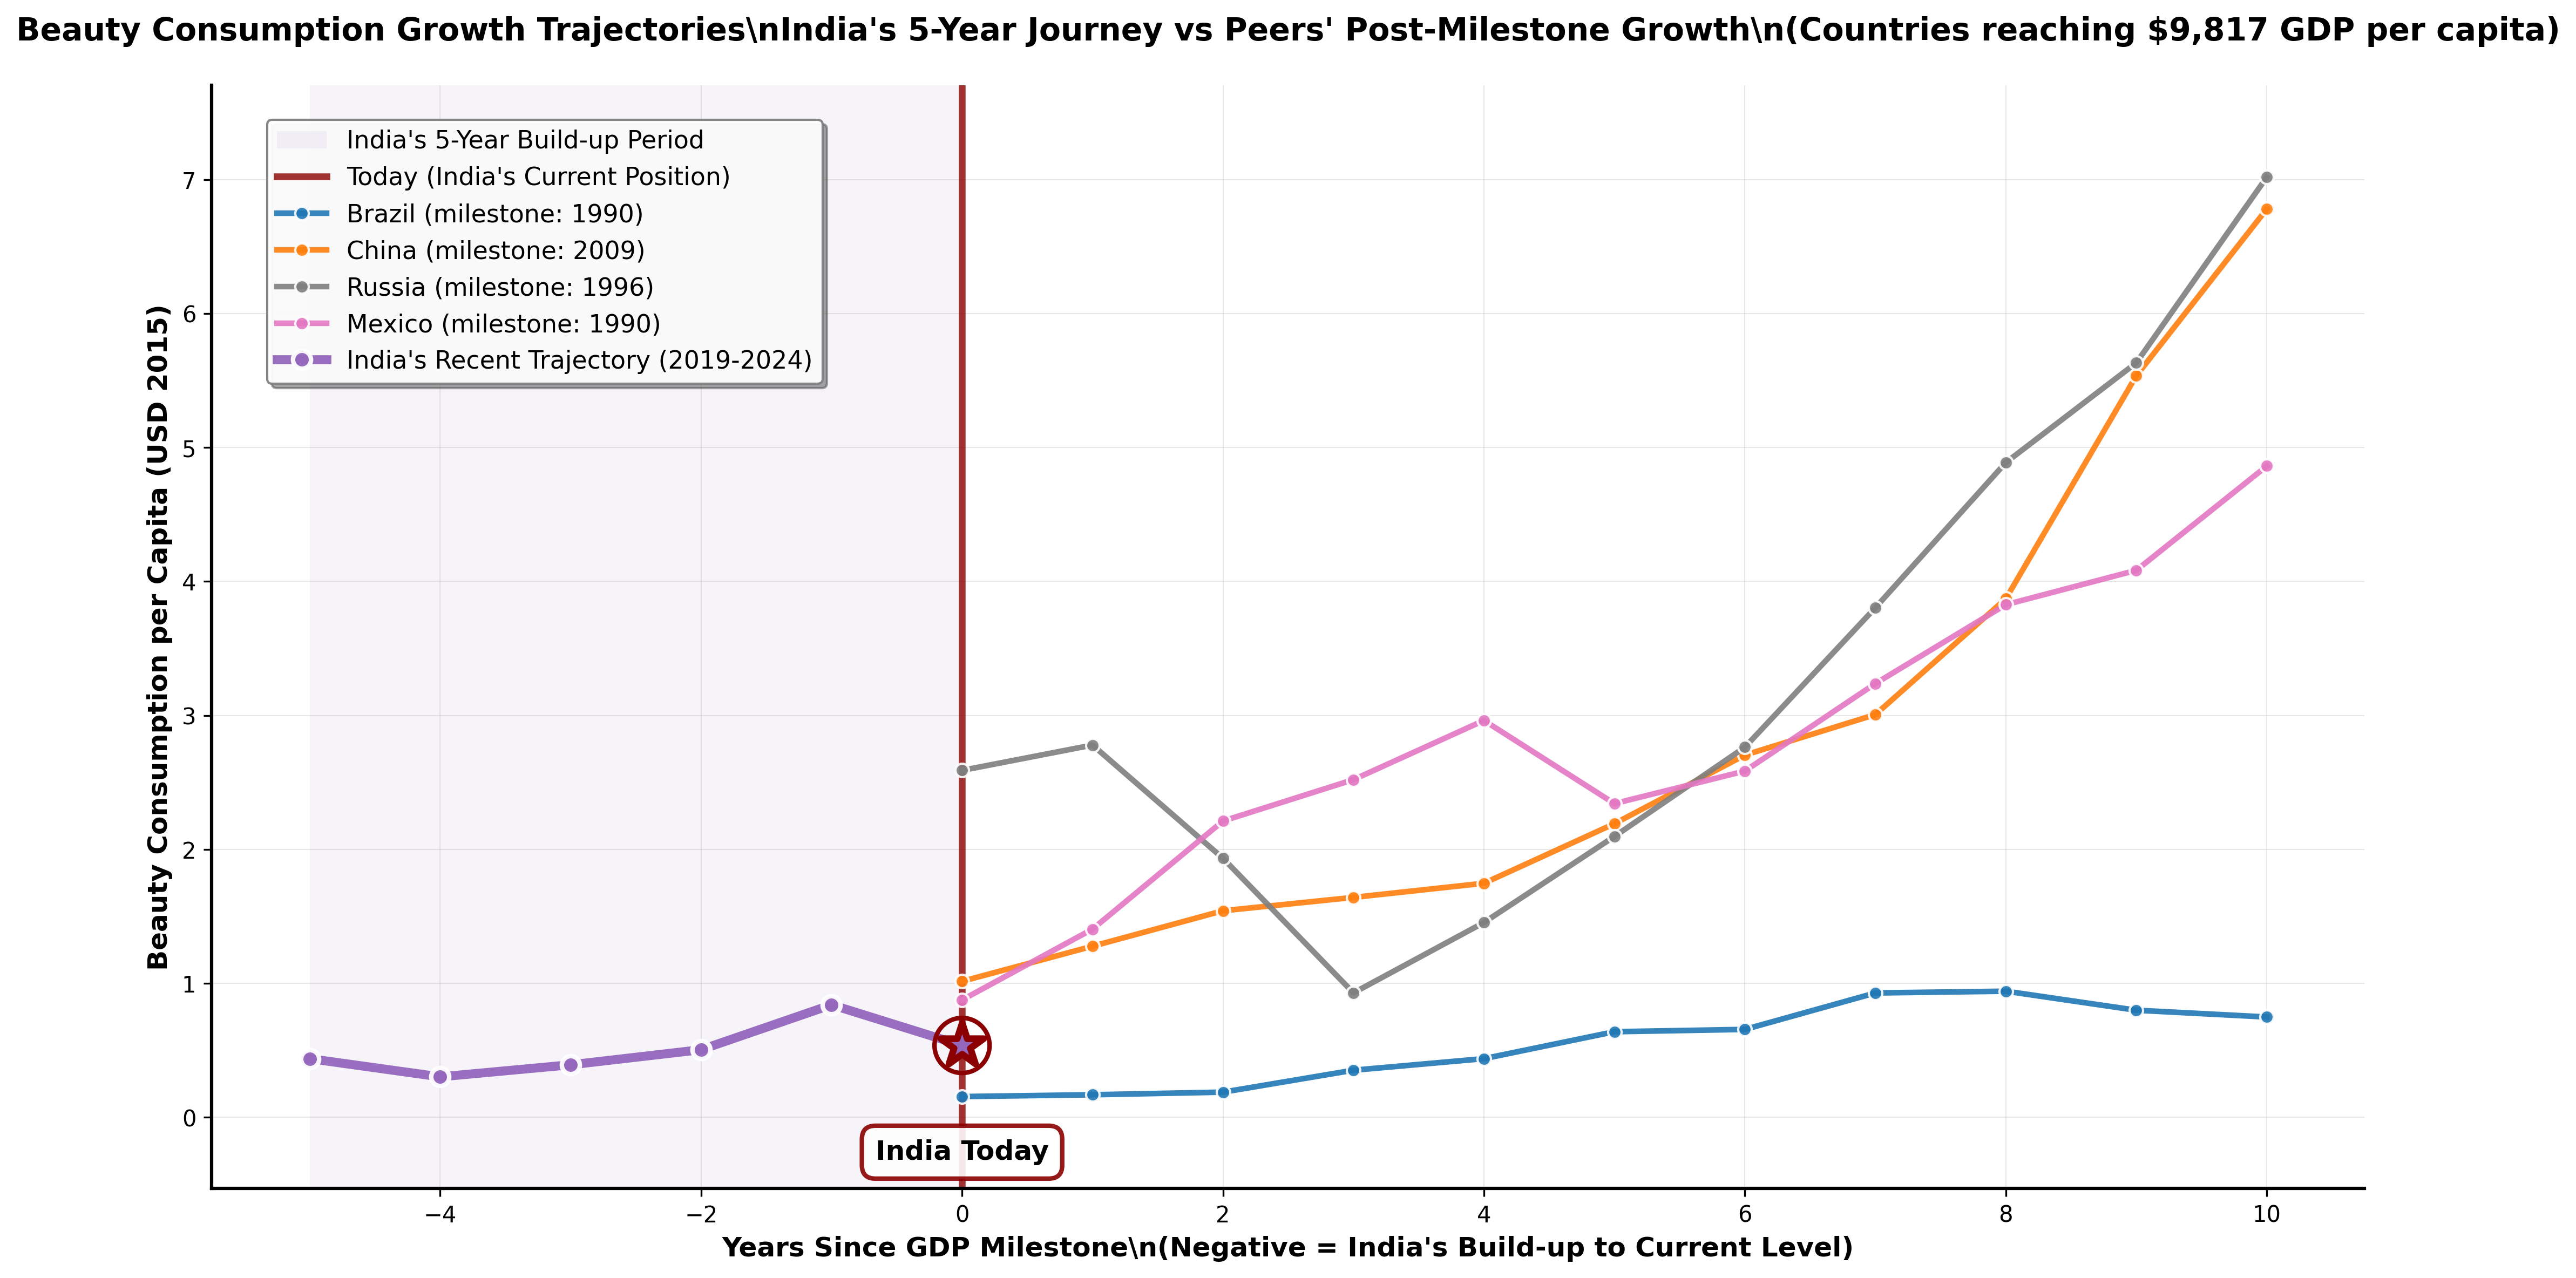
\includegraphics[width=0.8\textwidth]{T2-2_alignment_chart.png}
\caption{\textbf{Figure 7}: Income Alignment Methodology - Visual demonstration of how peer countries align with India's current development stage for fair growth comparisons}
\end{figure}

\textbf{Key Takeaways:}
\vspace{-3pt}
\begin{itemize}
    \setlength{\itemsep}{1pt}
    \item Significant growth gap suggests either unfavorable conditions or \textbf{substantial upside potential} if catalysts emerge
    \item Stable cluster membership indicates acceleration requires \textbf{external catalysts rather than natural progression}
    \item If India follows Brazil/Korea paths, expect 20-30\% growth rates, but current trajectory suggests this requires market development
\end{itemize}
\textit{See Appendix Section C for detailed methodology.}

% Task 3: Hypothesis Testing  
\section{Task 3: Hypothesis Testing}

\textbf{What We Did:} We statistically tested the hypothesis \textit{"Beauty consumption accelerates disproportionately once GDP crosses thresholds"} using piecewise regression and F-tests across beauty, skincare, men's wear, and women's wear for 11 countries, examining category-specific and gender-specific threshold effects.

\textbf{What the Numbers Show:}
\vspace{-3pt}
\begin{itemize}
    \setlength{\itemsep}{1pt}
    \item \textbf{Hypothesis statistically confirmed} with F-test results showing significant threshold effects (p-values well below conventional levels)
    \item Category analysis: Beauty overall (11 countries) - strong effects; \textbf{Skincare (11 countries) - strongest significance}; Men's wear (7 countries) - moderate; \textbf{Women's wear (7 countries) - strong}
    \item Slope change analysis shows skincare has most dramatic post-threshold acceleration
    \item Statistical robustness confirmed through bootstrap sampling (1,000 iterations)
\end{itemize}

\begin{figure}[H]
\centering
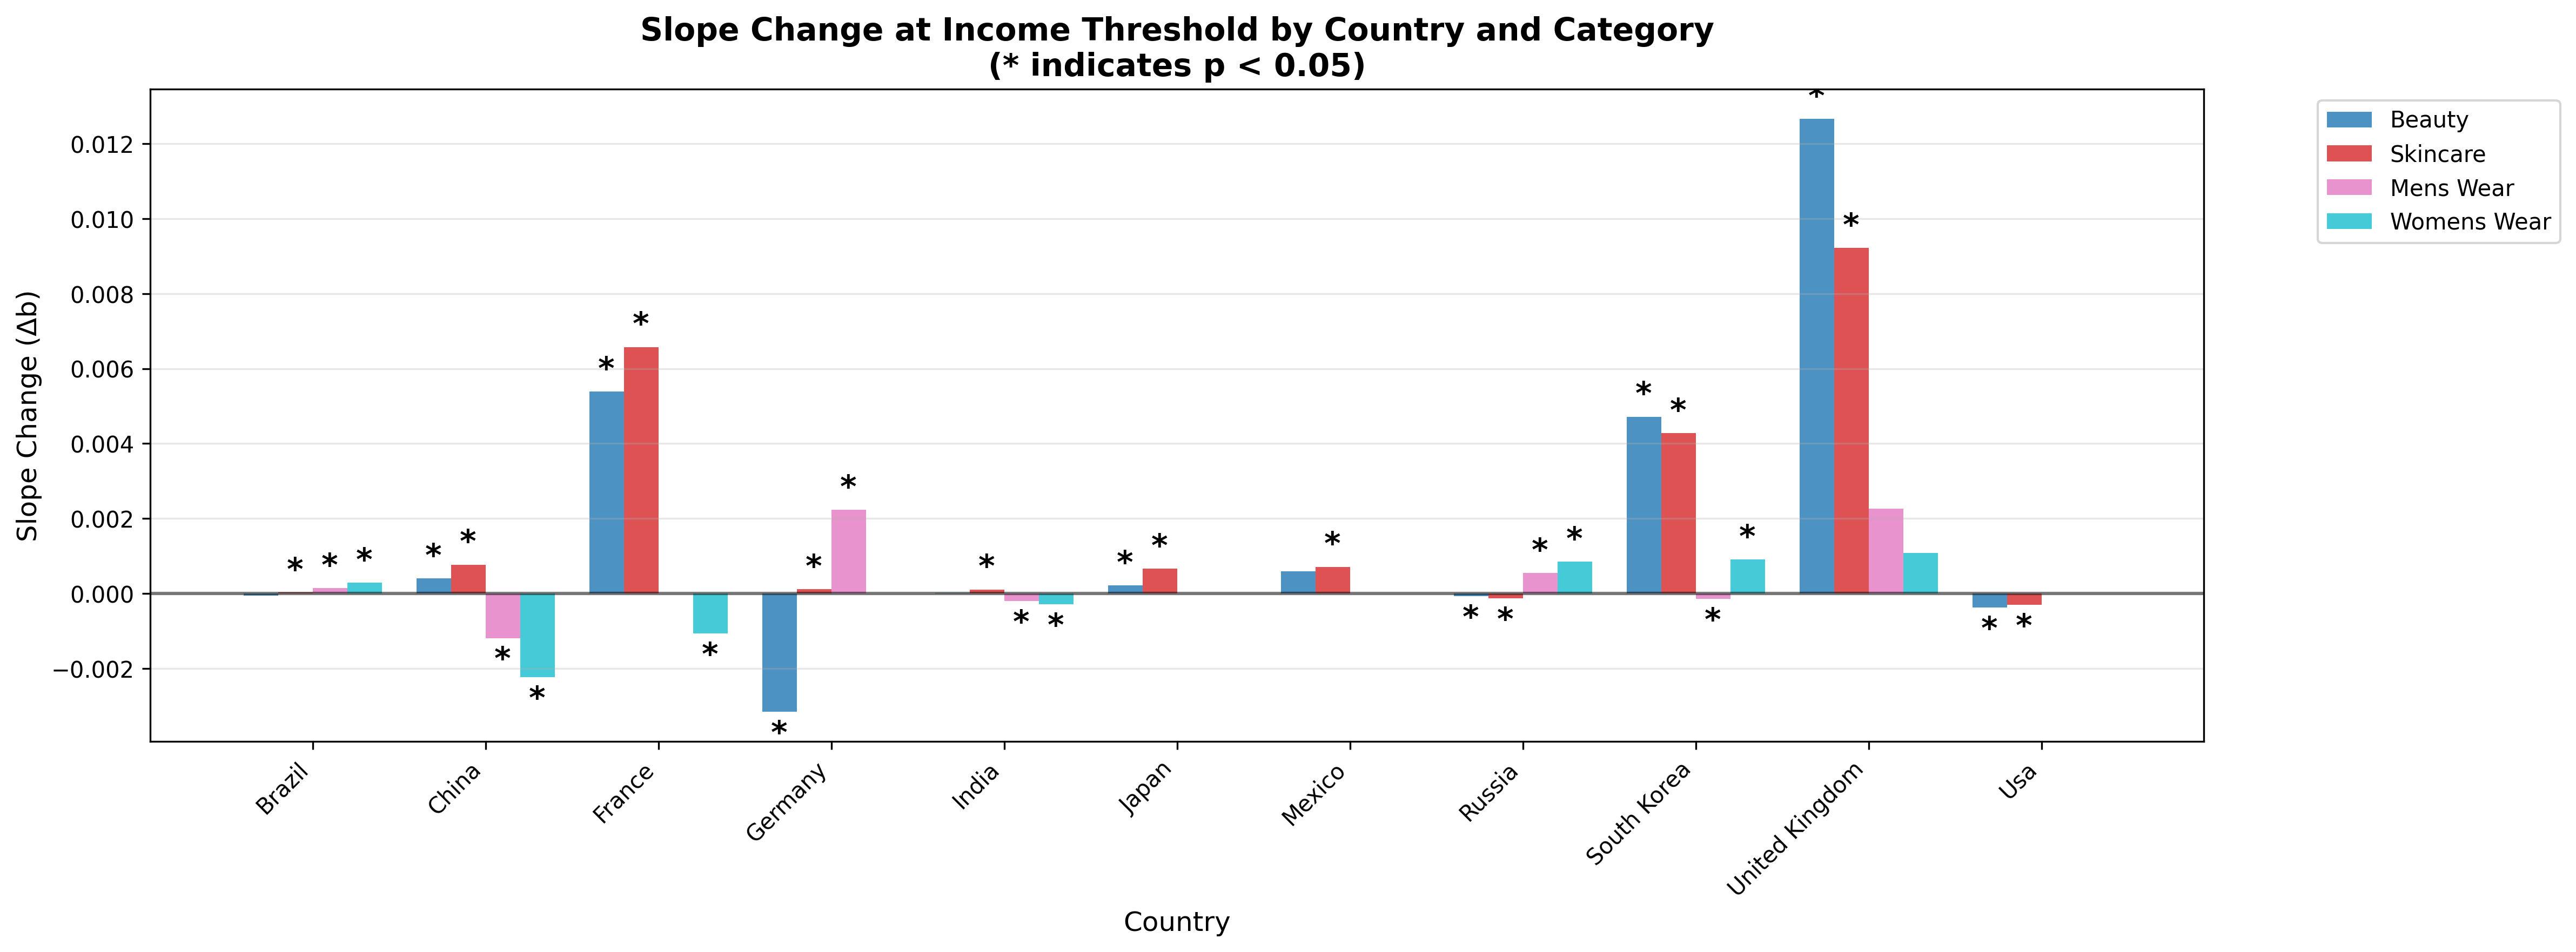
\includegraphics[width=0.7\textwidth]{HT-2_slope_change_bar_chart.png}
\caption{\textbf{Figure 8}: Slope Changes - Acceleration magnitude by category showing skincare and women's wear demonstrate strongest threshold effects}
\end{figure}


\textbf{Key Takeaways:}
\vspace{-3pt}
\begin{itemize}
    \setlength{\itemsep}{1pt}
    \item Statistical validation confirms acceleration is \textbf{predictable rather than random}, enabling evidence-based timing decisions
    \item Category insights guide allocation: \textbf{skincare offers highest growth potential} at thresholds
    \item Women's beauty shows stronger threshold effects than men's, indicating female-focused strategies more responsive in emerging markets
    \item Consistent threshold clustering around \$40-50k provides \textbf{clear target benchmarks for market acceleration timing}
\end{itemize}
\textit{Note: Countries with R² < 0.3 excluded for reliability.} \textit{See Appendix Section D for detailed statistical significance testing results and F-test confidence levels.}

% India vs Peers: Investment Positioning Analysis
\section{India vs Peers: Investment Positioning Analysis}

India sits at \textbf{\$8,563 GDP per capita}, well below the \$40-50k threshold where acceleration typically occurs. However, \textbf{relative to income-matched peers}, India significantly underperforms—countries at similar stages historically achieved 15-35\% growth rates vs India's 4.1\%.

\textbf{Korean Beauty Parallel:} South Korea's transformation provides relevant precedent. Korea's acceleration began at similar relative positioning to India today, demonstrating \textbf{catalyst-driven growth can precede natural income progression}. Cultural factors, digital adoption, and behavioral shifts created breakouts independent of traditional thresholds.

\textbf{Investment Implications:} Conservative assessment suggests longer horizons given below-threshold positioning. However, the significant peer performance gap indicates \textbf{substantial upside potential} if catalysts emerge. Digital penetration and demographic shifts could drive acceleration ahead of traditional income progression. Priority segments: \textbf{skincare and women's wear} show strongest threshold effects. 

\textit{Note: Detailed clustering analysis of India's market positioning relative to growth patterns is provided in Appendix Section C. Conservative models suggest 10-15 years for natural threshold crossing; catalyst scenarios indicate 5-7 years with targeted market development.}

\newpage

% Appendix
\section*{Appendix: Comprehensive Analysis Documentation}
\addcontentsline{toc}{section}{Appendix: Comprehensive Analysis Documentation}

\subsection*{Section A: Data Sources \& Methodology}

\textbf{Data Sources \& Definitions}

\textbf{Economic Indicators}: World Bank data including GDP per capita (PPP, constant 2021 international \$) and household final consumption expenditure per capita (constant 2015 US\$). These provide standardized, internationally comparable measures of economic development and consumption capacity.

\textbf{Beauty Product Data}: UN Comtrade data covering HS codes 3303-3307 (perfumes, cosmetics, skincare products) plus apparel categories 6101-6104 and 6203-6204 for men's and women's wear analysis. Trade flow data serves as proxy for consumption patterns.

\textbf{Country Coverage}: 11 countries analyzed (Brazil, China, France, Germany, India, Japan, Mexico, Russia, South Korea, United Kingdom, USA) selected for data availability and economic diversity.

\textbf{Analytical Approaches \& Rationale}

\textbf{Income Elasticity Analysis}: Log-log regression models measuring consumption responsiveness to income changes. \textit{Rationale}: This approach enables identification of luxury vs necessity goods through elasticity coefficients—values >1 indicate luxury behavior where consumption grows faster than income. The log-log specification linearizes power relationships common in economic data.

\textbf{Piecewise Regression}: Structural break detection using iterative fitting across potential threshold points. \textit{Rationale}: We suspected consumption patterns change at specific income levels rather than following smooth curves. Piecewise regression identifies these breakpoints statistically, enabling threshold-based investment strategies rather than assuming linear relationships.

\textbf{Peer Income Matching}: Historical analysis matching countries at similar GDP per capita levels. \textit{Rationale}: Direct comparison of current India vs developed countries would be misleading due to income differences. Matching historical periods enables fair comparison of growth trajectories at similar development stages.

\textbf{Statistical Testing}: F-tests for threshold significance, bootstrap sampling for confidence intervals (1,000 iterations), R² thresholds (>0.3) for analytical inclusion. \textit{Rationale}: Investment decisions require statistical confidence, not just visual patterns. F-tests validate threshold significance, bootstrap sampling provides robust confidence intervals, and R² thresholds ensure reliable relationships.

\textbf{Key Limitations \& Tradeoffs}

\textit{Trade Data as Consumption Proxy}: UN Comtrade captures import/export flows rather than direct consumption, potentially missing domestic production and informal markets. However, this approach provides standardized cross-country comparability unavailable in direct consumption surveys.

\textit{Developed Market Saturation}: Some developed countries show weak income-consumption relationships, particularly for apparel categories, as consumption may be driven by replacement cycles rather than income growth.

\textit{Time Period Constraints}: Analysis covers available data periods which vary by country, potentially affecting trend detection in countries with limited historical data.

\textit{Category Aggregation}: Beauty product categories aggregate diverse subcategories with potentially different consumption patterns, though this enables higher-level strategic analysis.

\subsection*{Section B: Task 1 Statistical Exploration - Additional Charts}

\textbf{Complete statistical analysis supporting income elasticity findings and threshold detection.}


\begin{figure}[H]
\centering
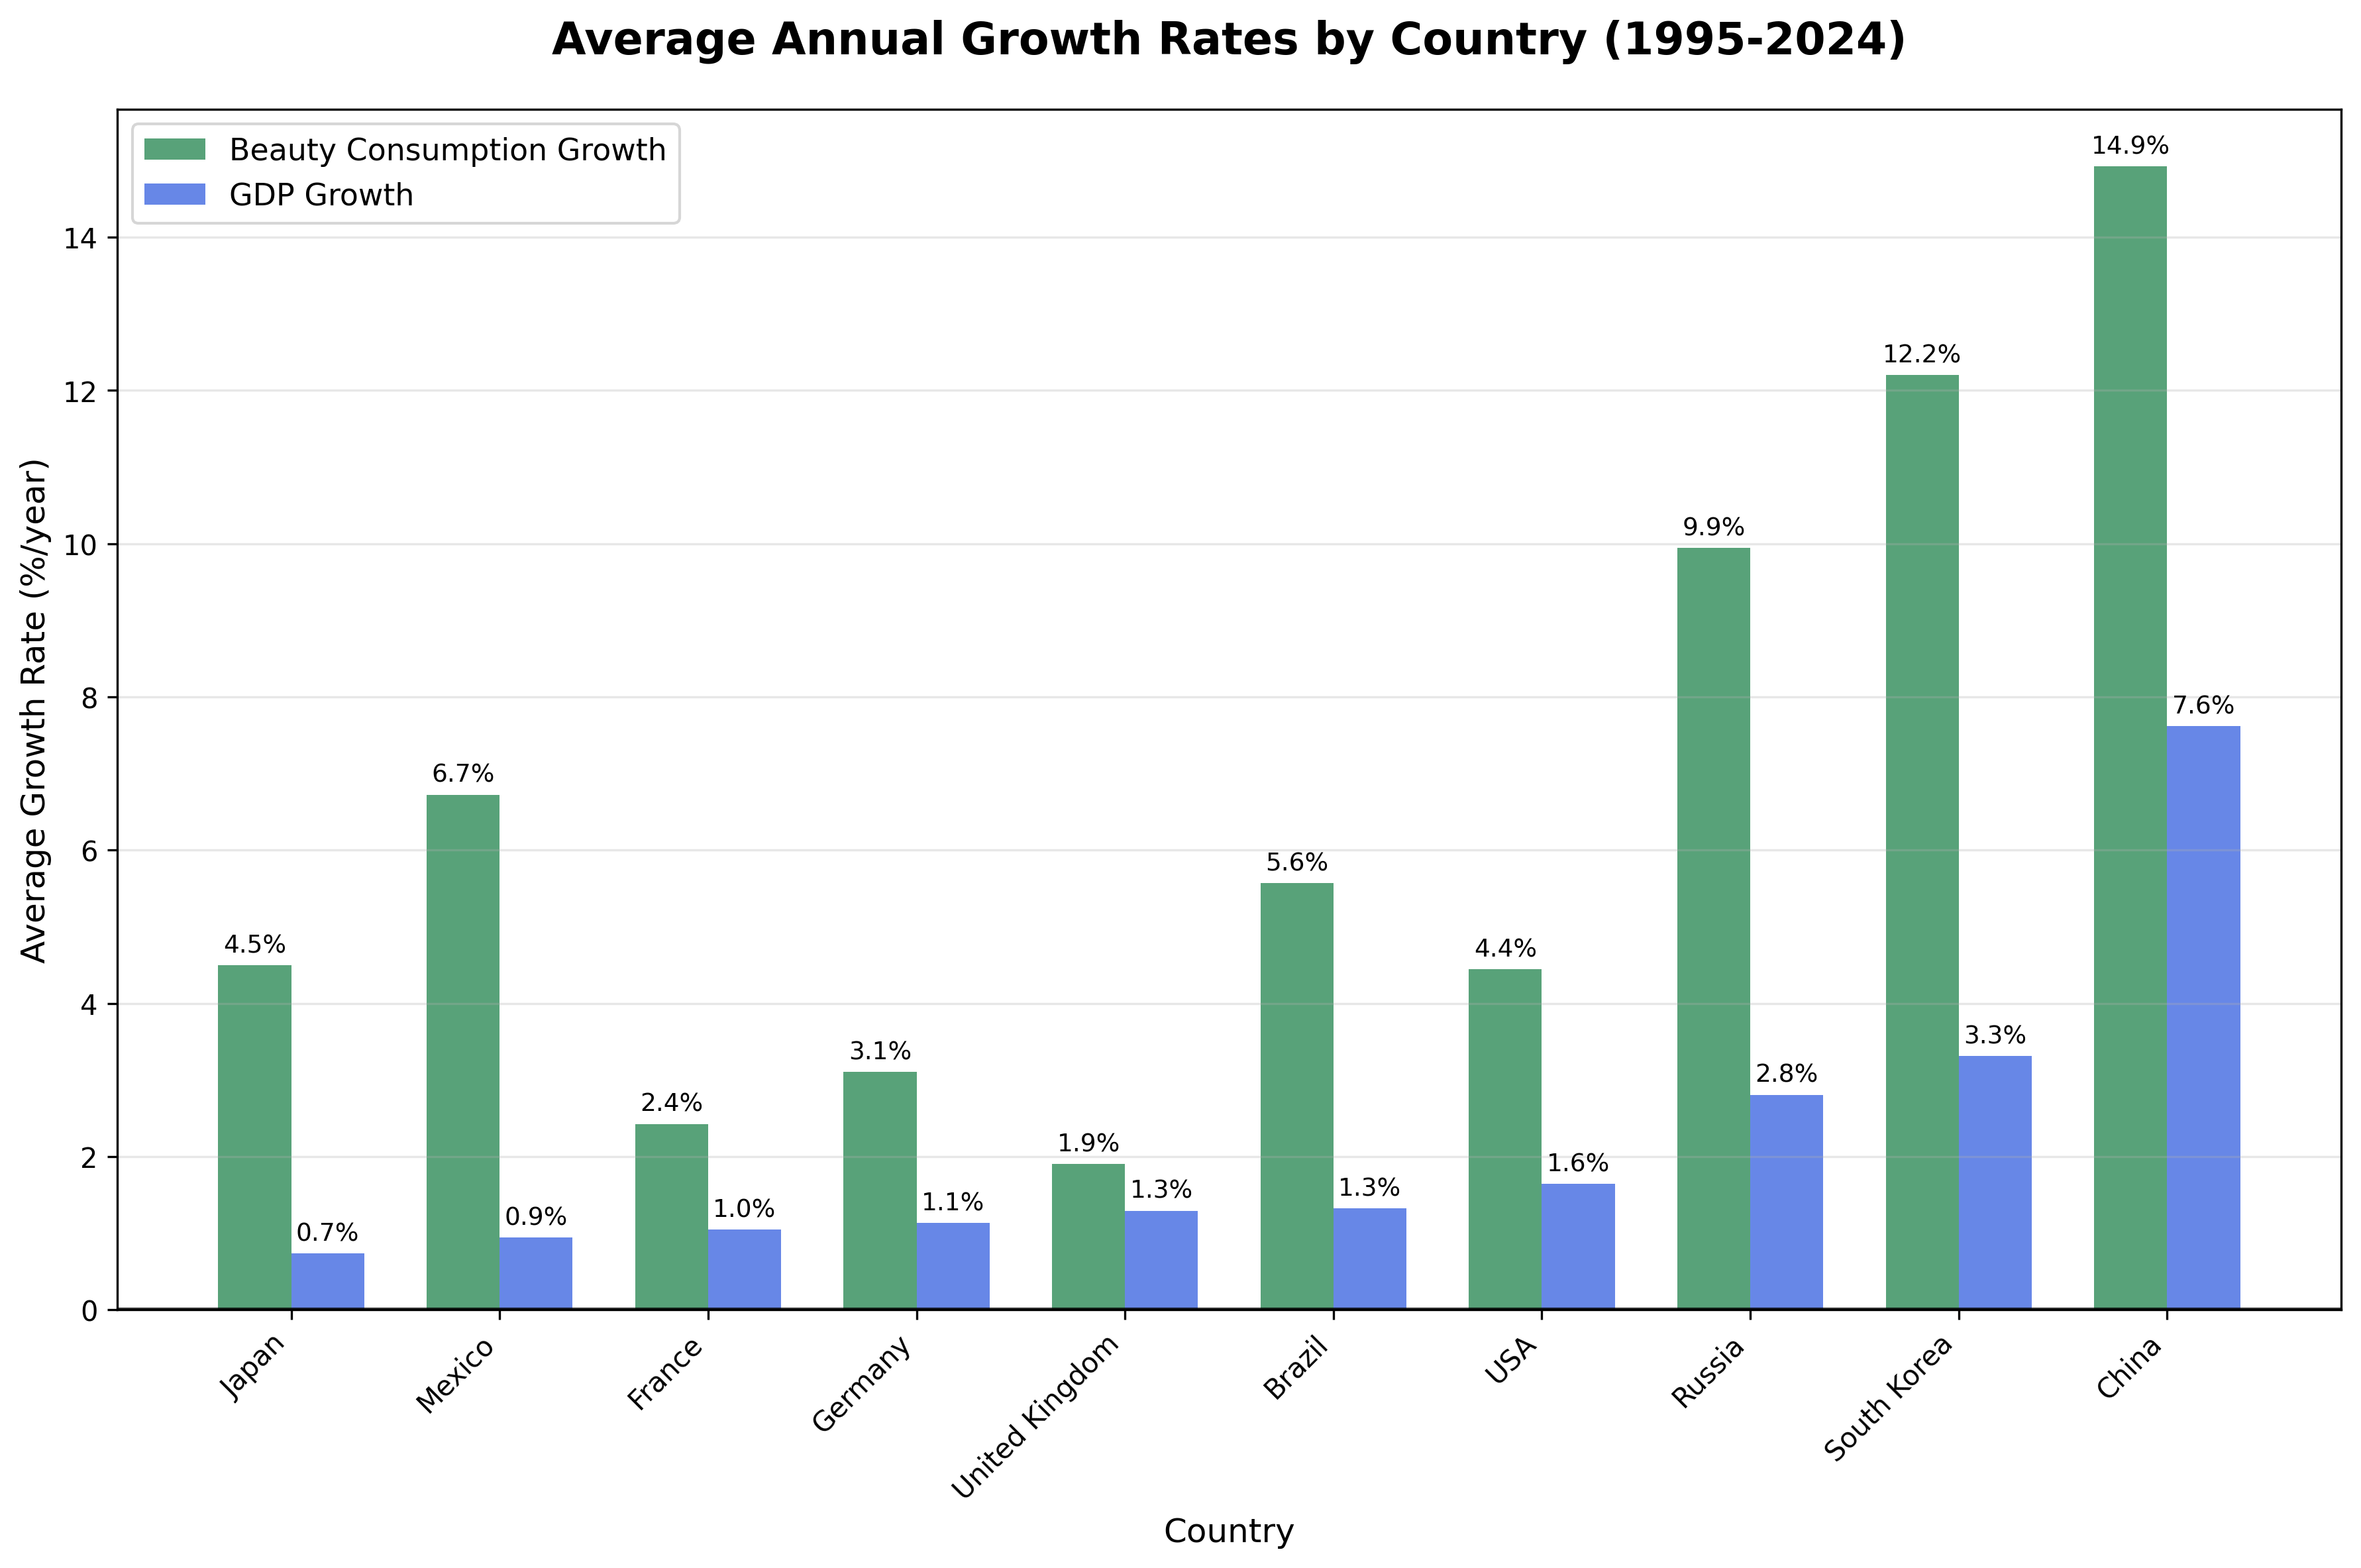
\includegraphics[width=0.8\textwidth]{T1-2_average_growth_rates_comparison.png}
\caption{\textbf{Figure A.1}: Average Growth Rates Comparison - Cross-country analysis of beauty consumption growth rates, showing variance in development patterns across different economic contexts.}
\end{figure}

\begin{figure}[H]
\centering
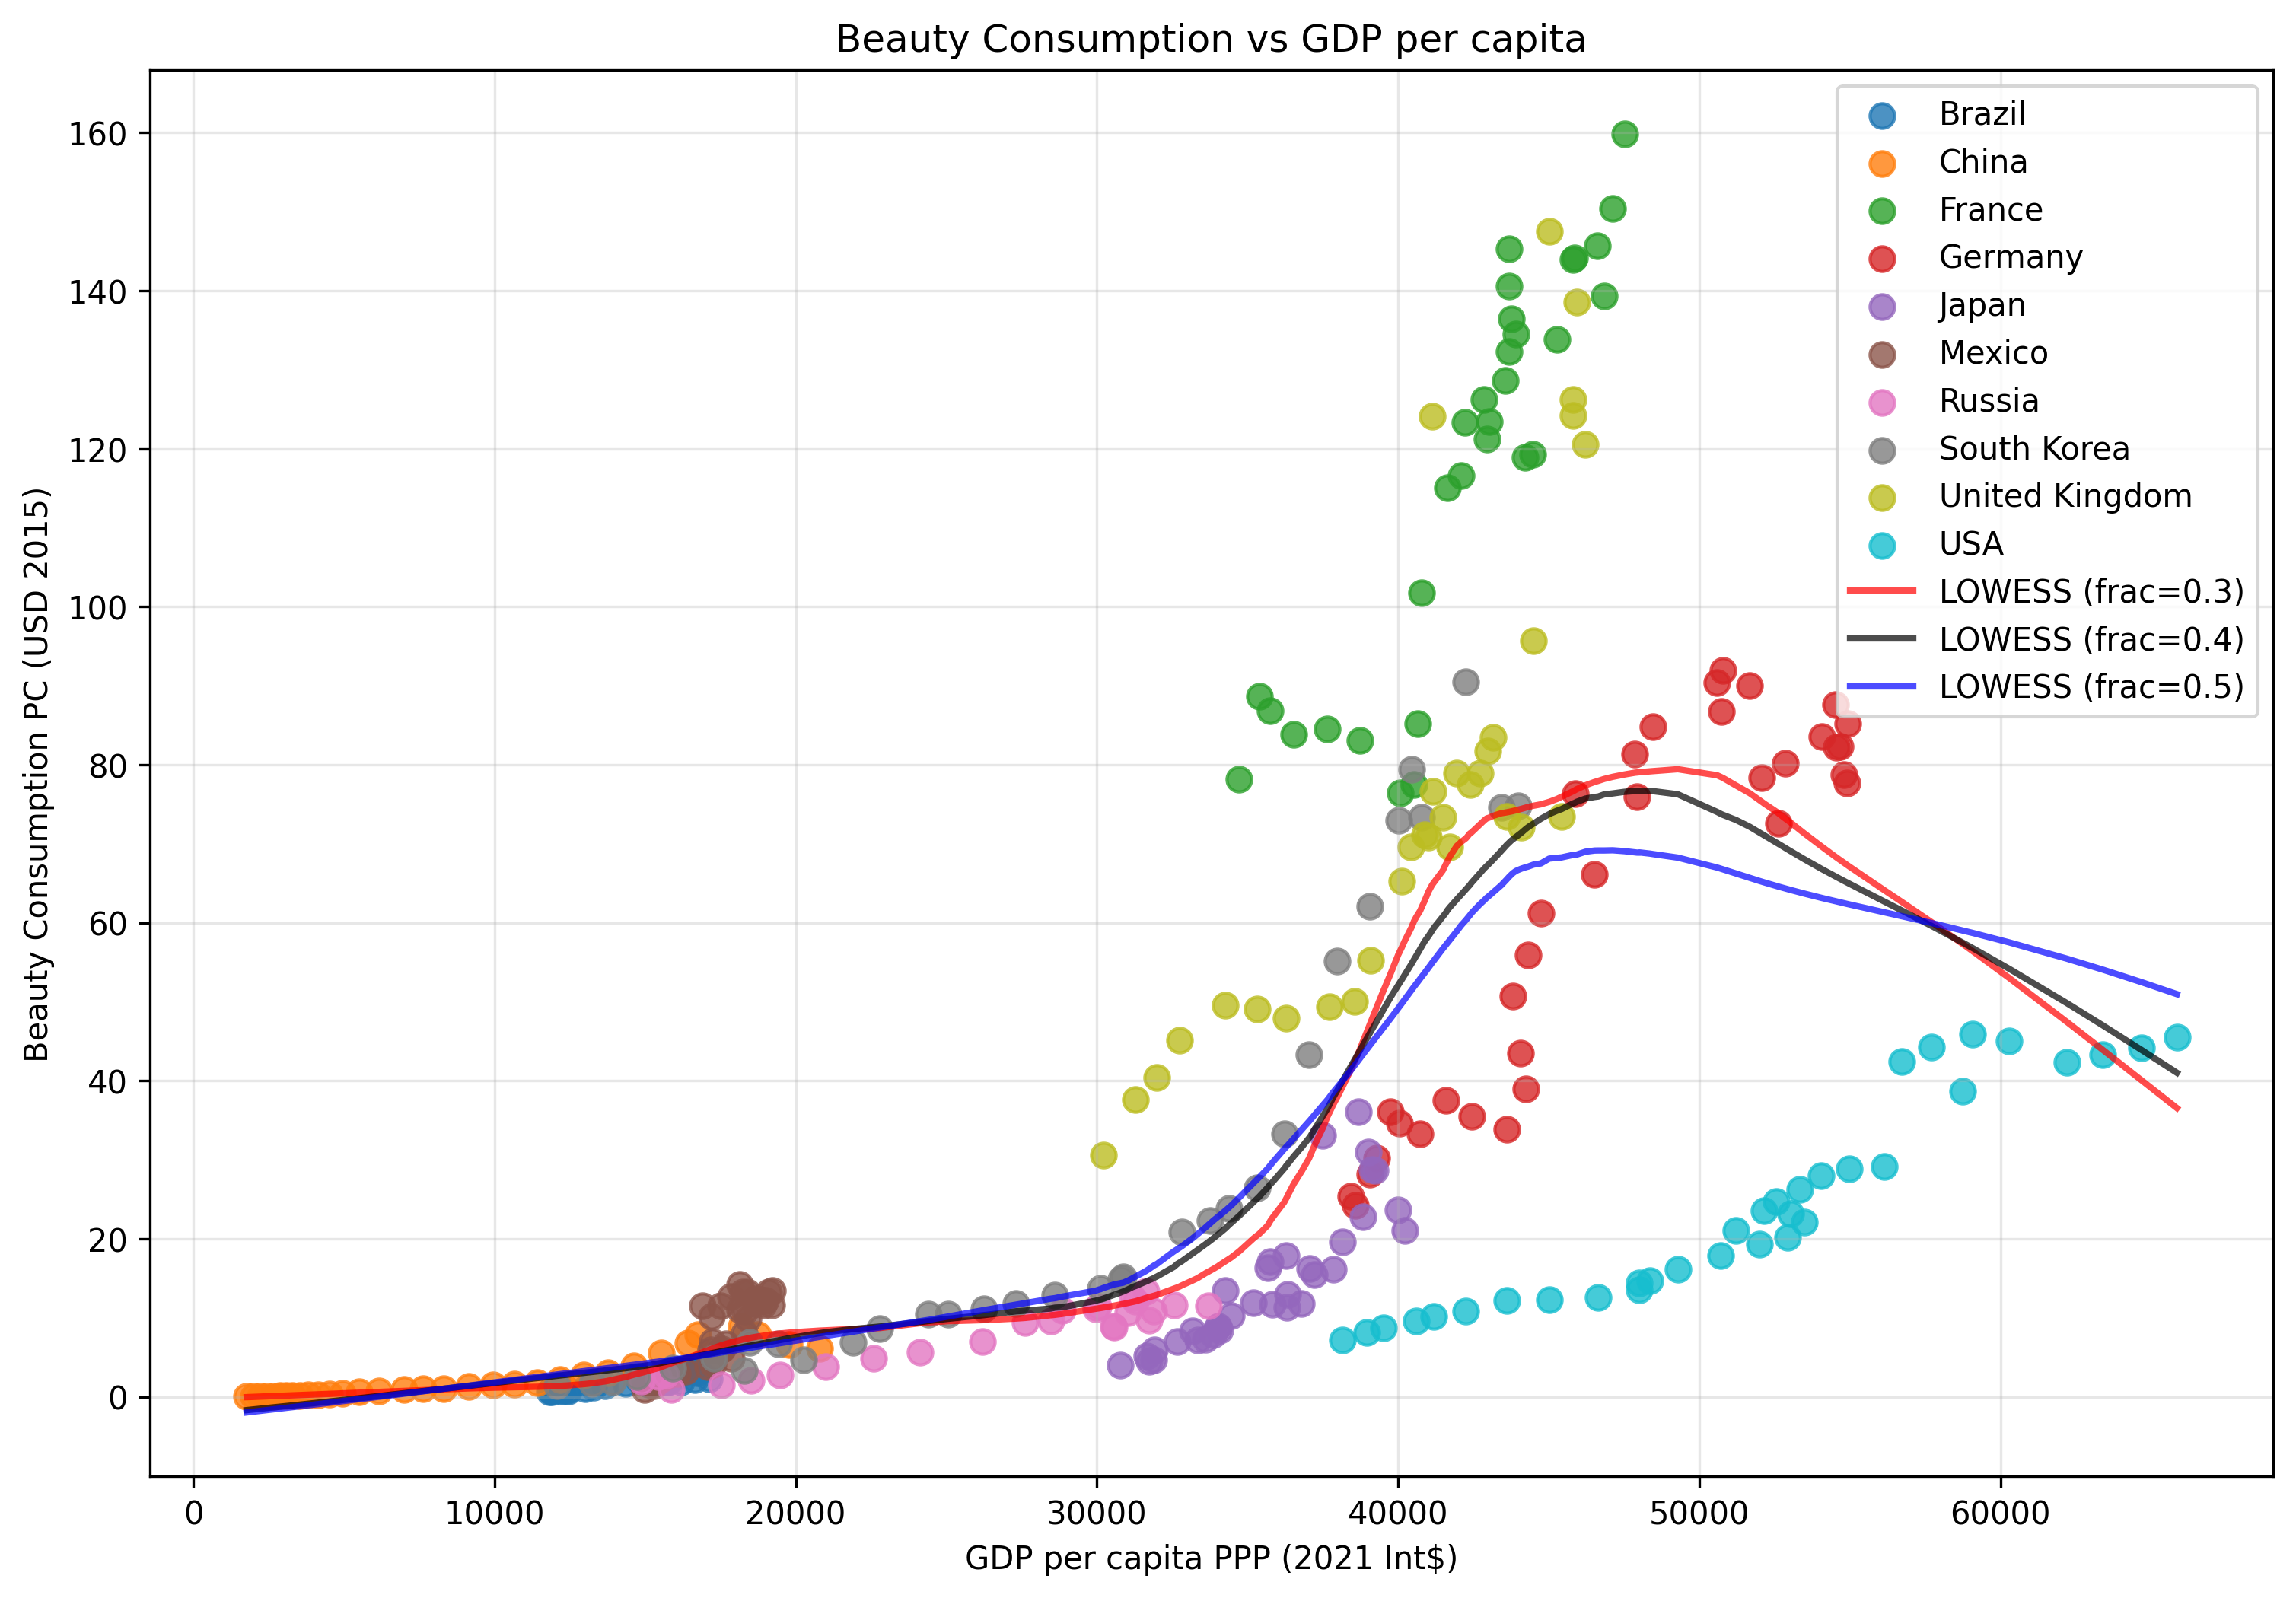
\includegraphics[width=0.8\textwidth]{T1-3_BeautyPC_vs_gdppcppp_scatter.png}
\caption{\textbf{Figure A.2}: Beauty Per Capita vs GDP Scatter - Raw scatter plot showing relationship between income and beauty consumption across all countries and time periods.}
\end{figure}

\begin{figure}[H]
\centering
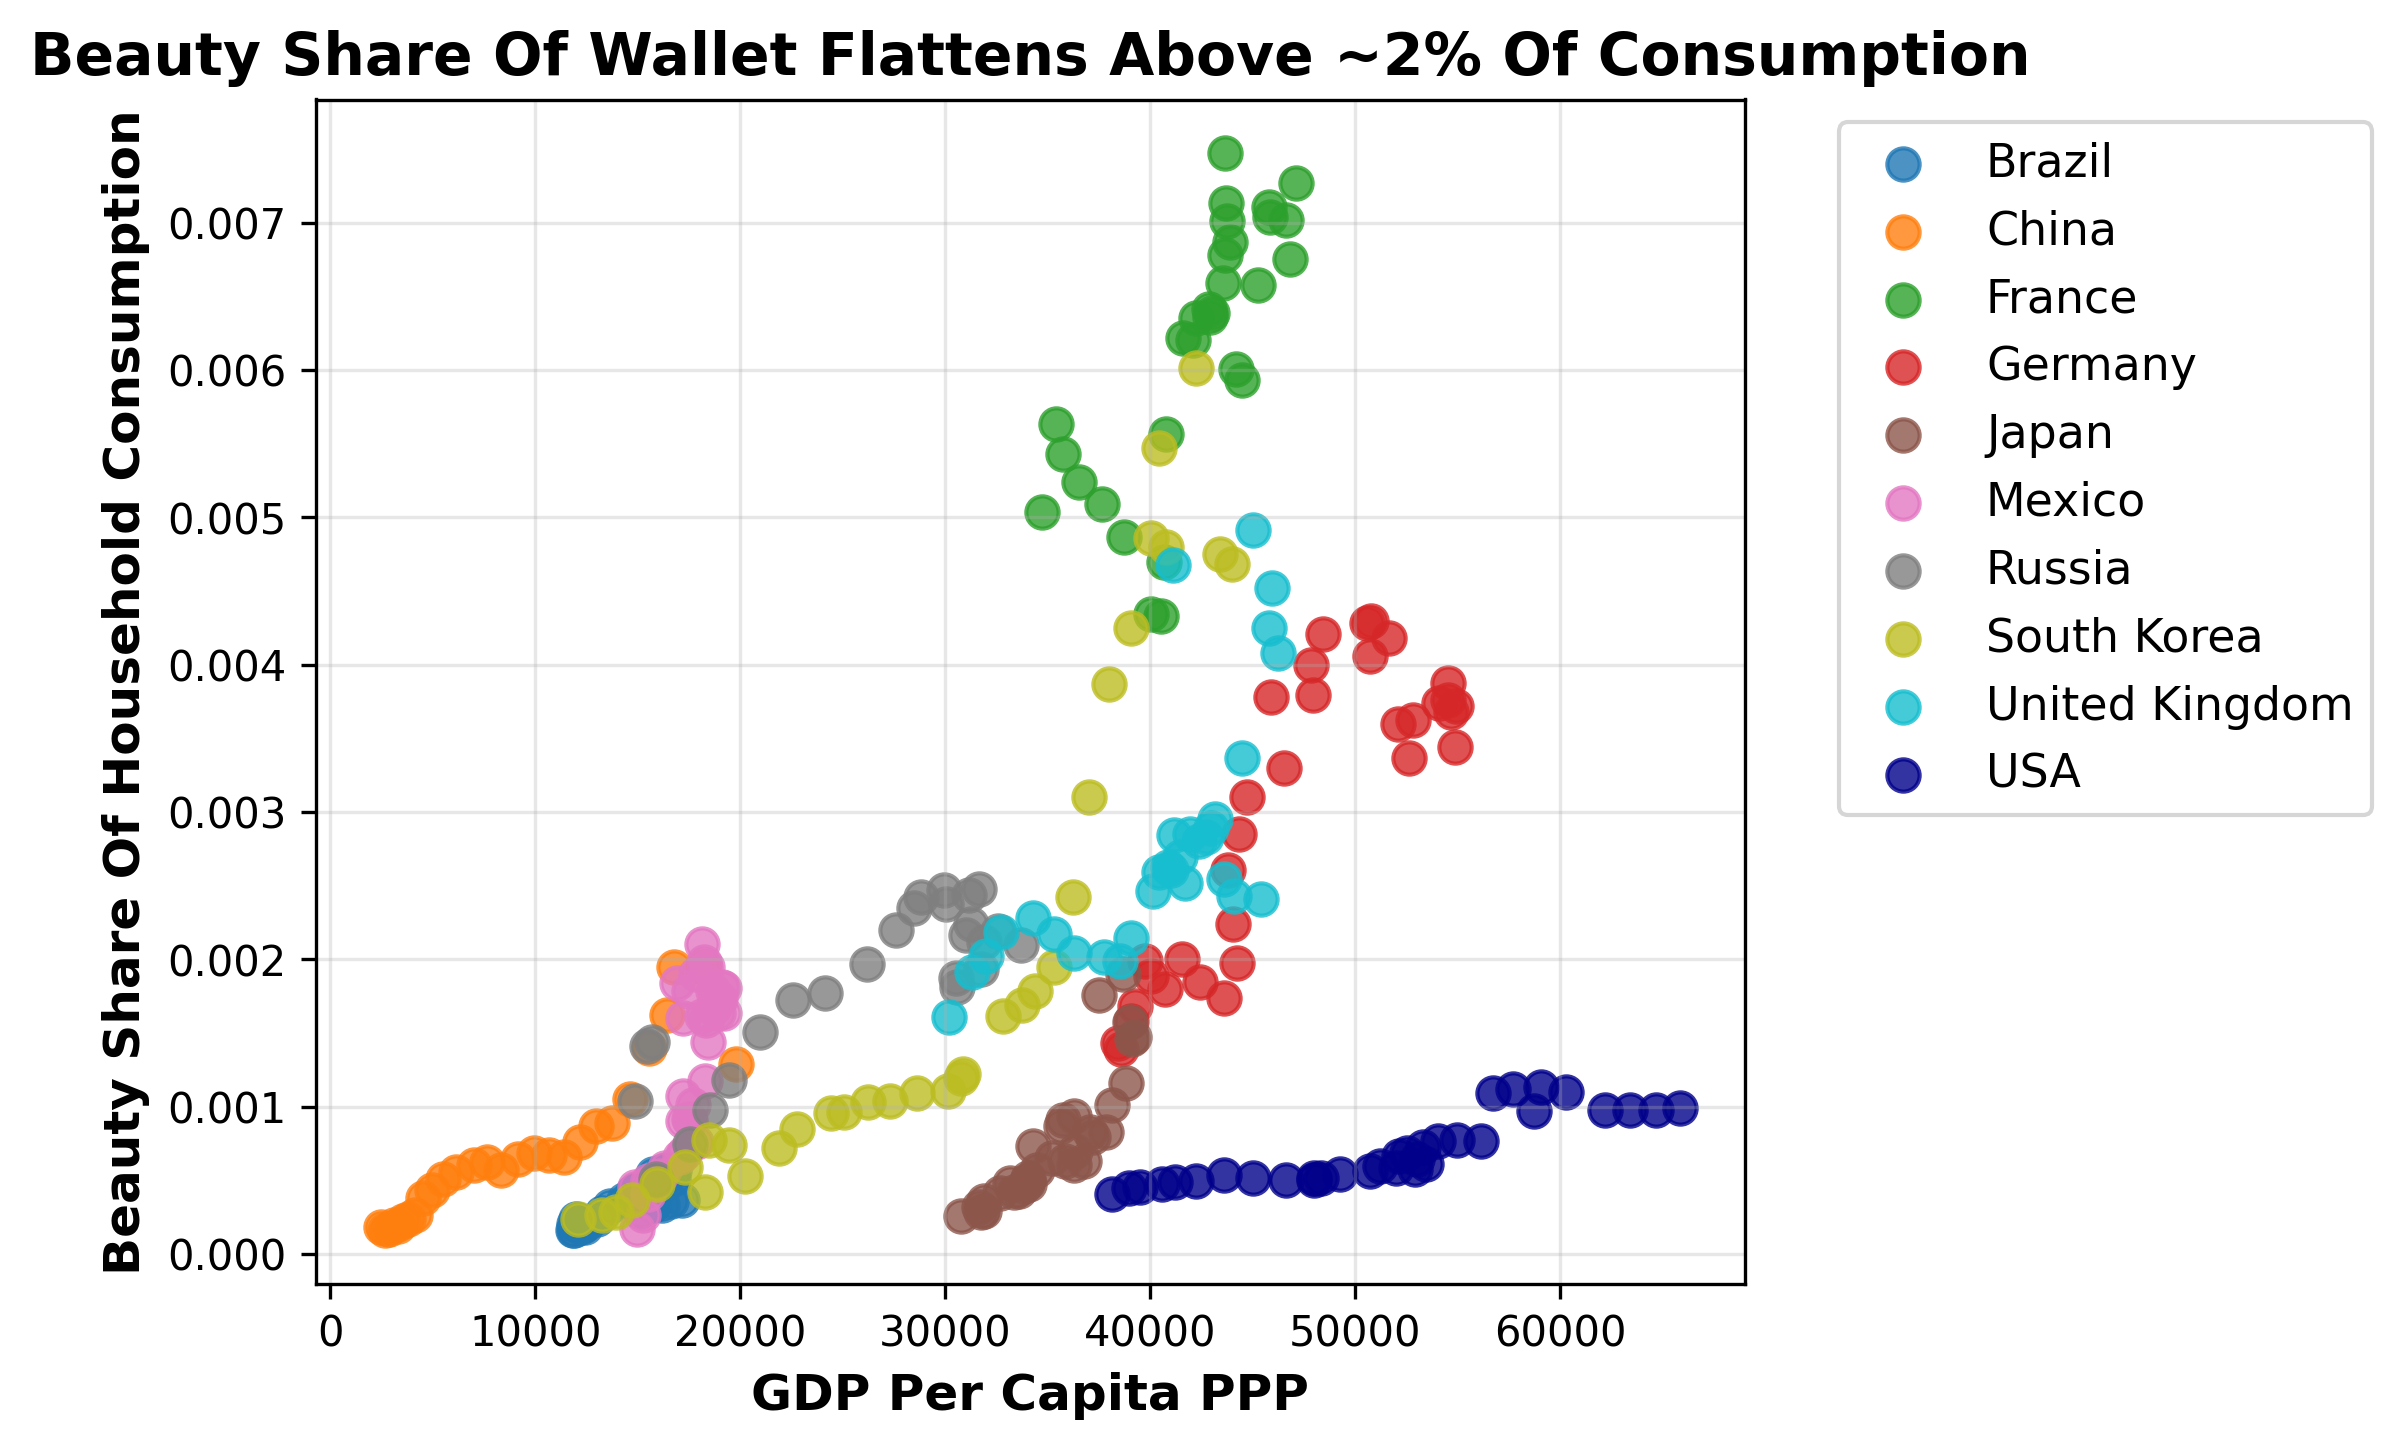
\includegraphics[width=0.8\textwidth]{T1-5_BeautyShare_vs_gdppcppp.png}
\caption{\textbf{Figure A.3}: Beauty Share vs GDP Analysis - Beauty consumption as percentage of total consumption, illustrating how beauty's share of wallet changes with income levels.}
\end{figure}


\subsection*{Section C: Task 2 Comparative Benchmarking - Additional Analysis}

\textbf{Detailed peer matching methodology and growth pattern analysis supporting India positioning assessment.}


\begin{figure}[H]
\centering
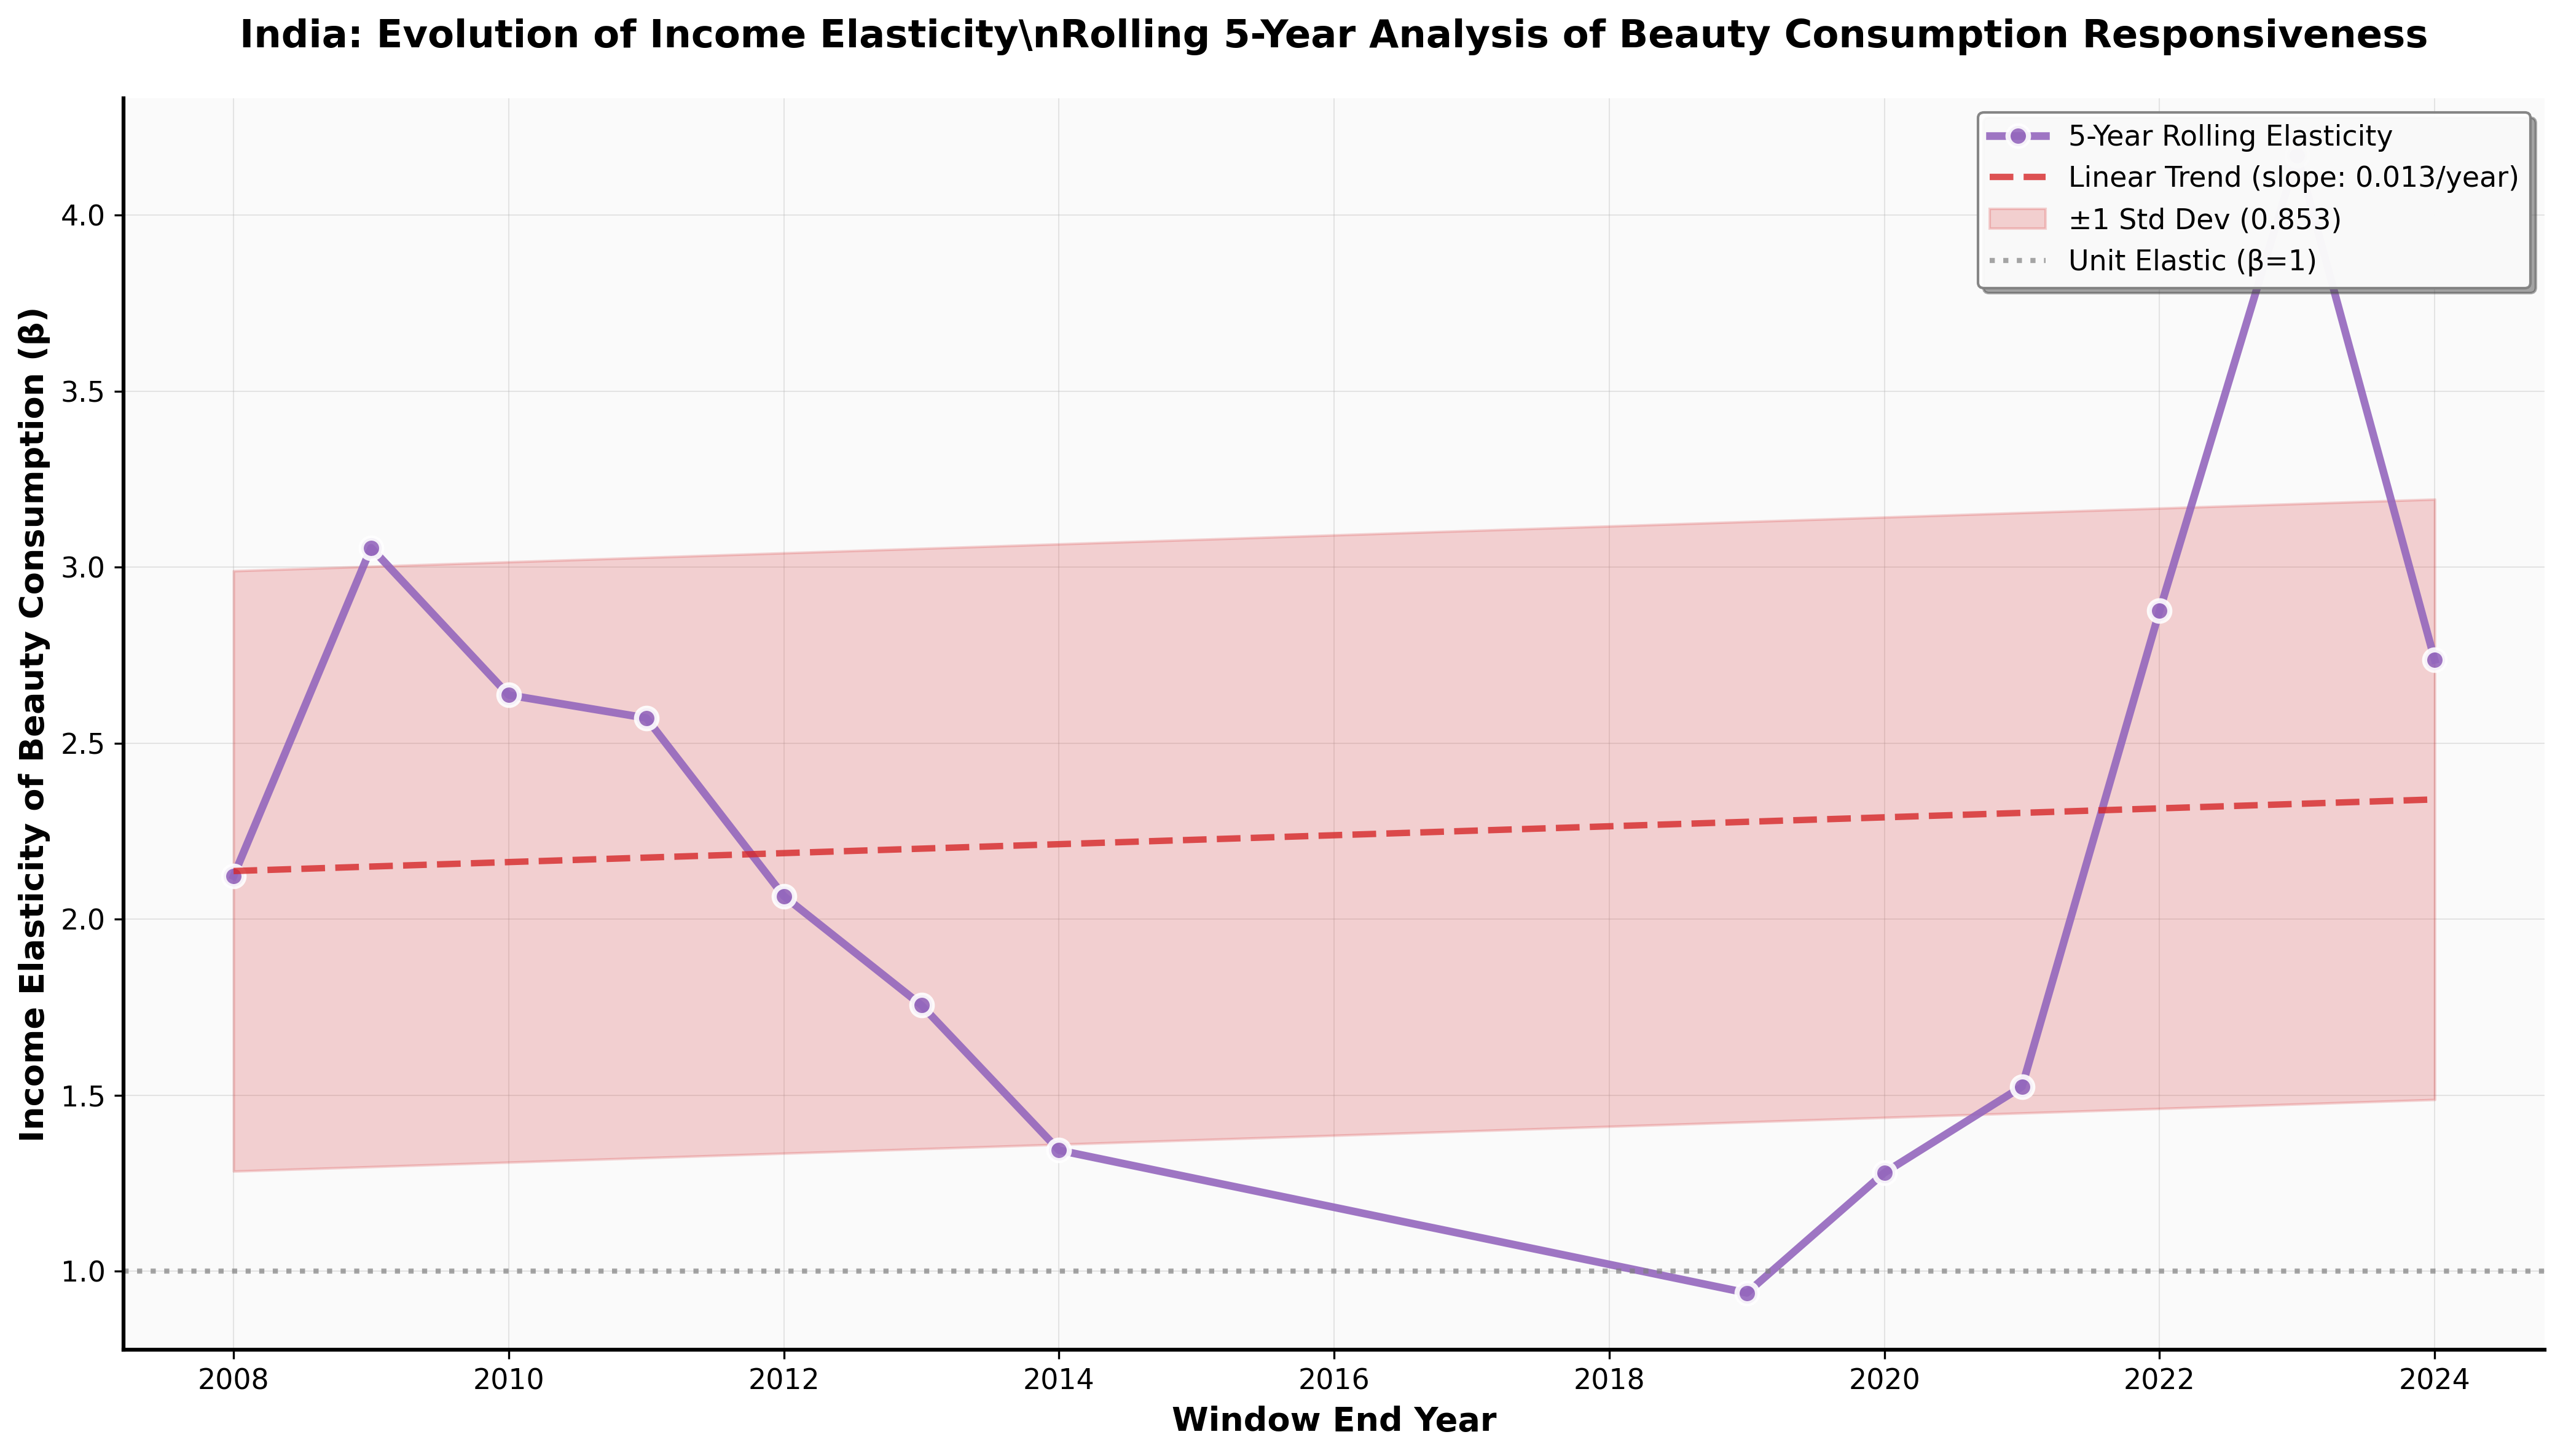
\includegraphics[width=0.8\textwidth]{T2-4_rolling_elasticity_india.png}
\caption{\textbf{Figure B.1}: Rolling Elasticity Analysis for India - Time-varying income elasticity calculations showing how India's consumption responsiveness has evolved over different periods.}
\end{figure}

\begin{figure}[H]
\centering
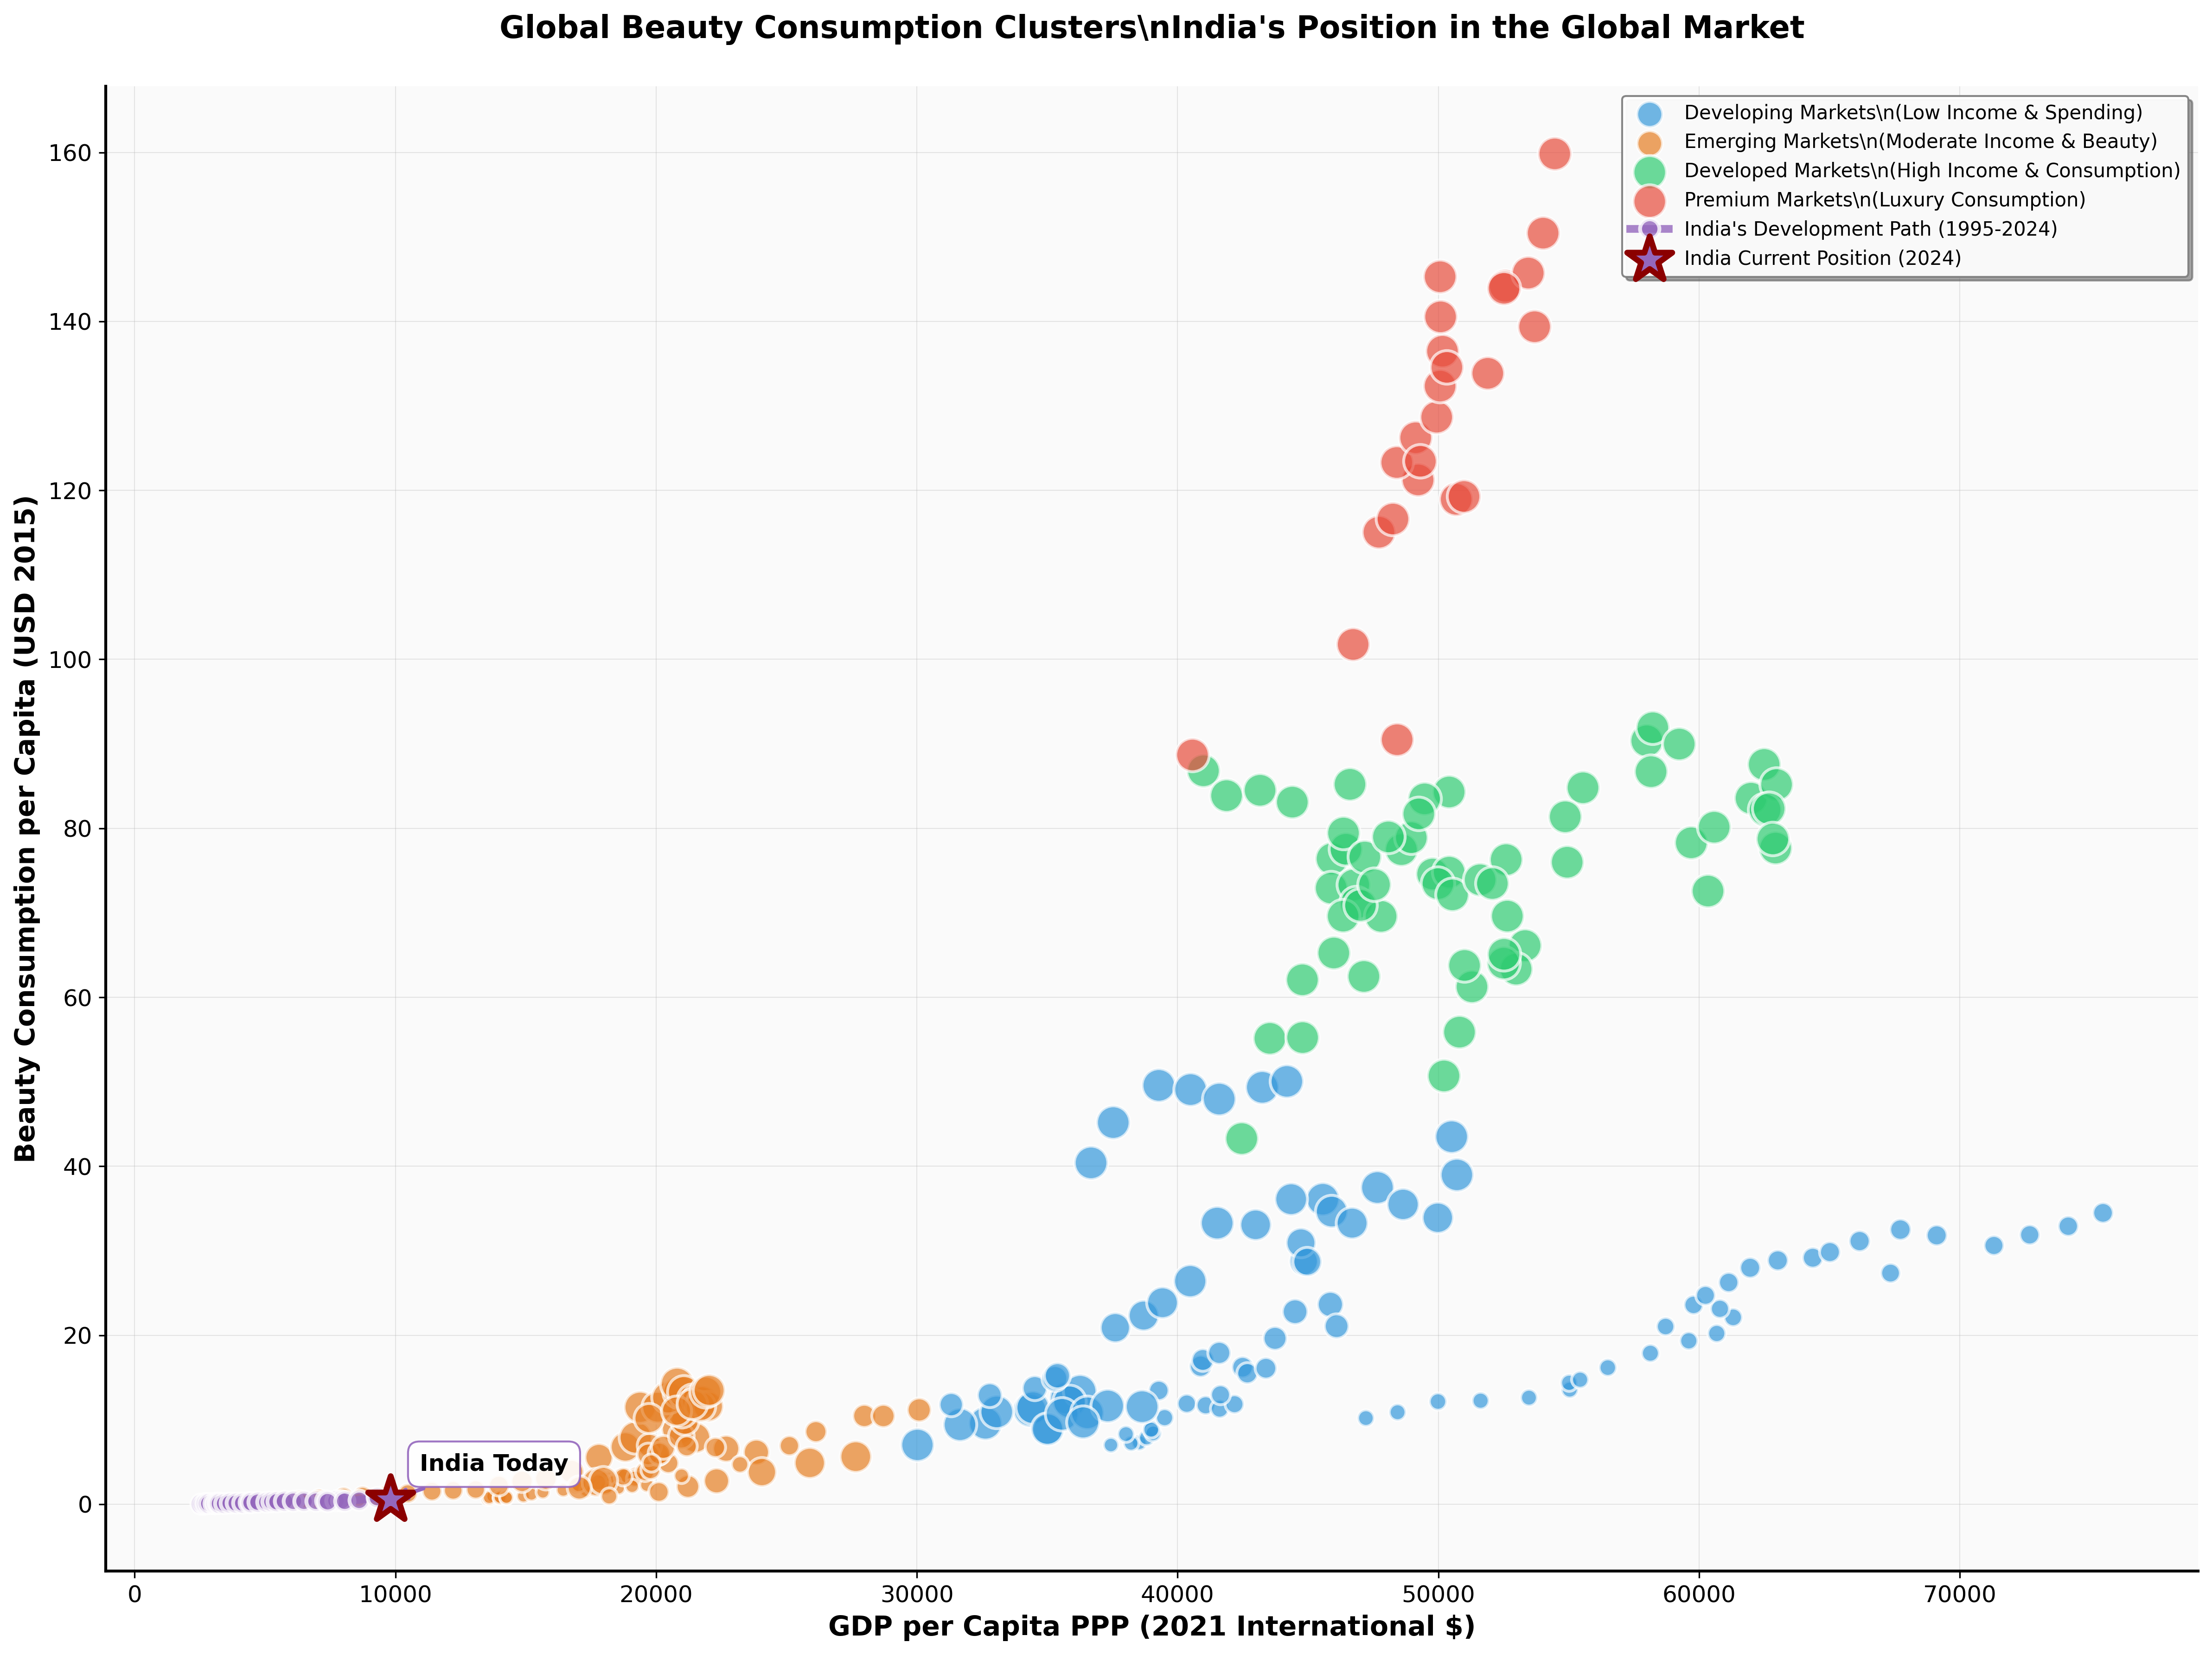
\includegraphics[width=0.8\textwidth]{T2-5_kmeans_scatter.png}
\caption{\textbf{Figure B.2}: K-Means Clustering Analysis - Statistical clustering of countries based on growth patterns, illustrating India's position in stable, lower-growth segment with potential for catalyst-driven acceleration to higher-growth clusters.}
\end{figure}

\subsection*{Section D: Task 3 Hypothesis Testing - Statistical Evidence}

\textbf{Comprehensive hypothesis testing results across all categories and countries.}

\begin{figure}[H]
\centering
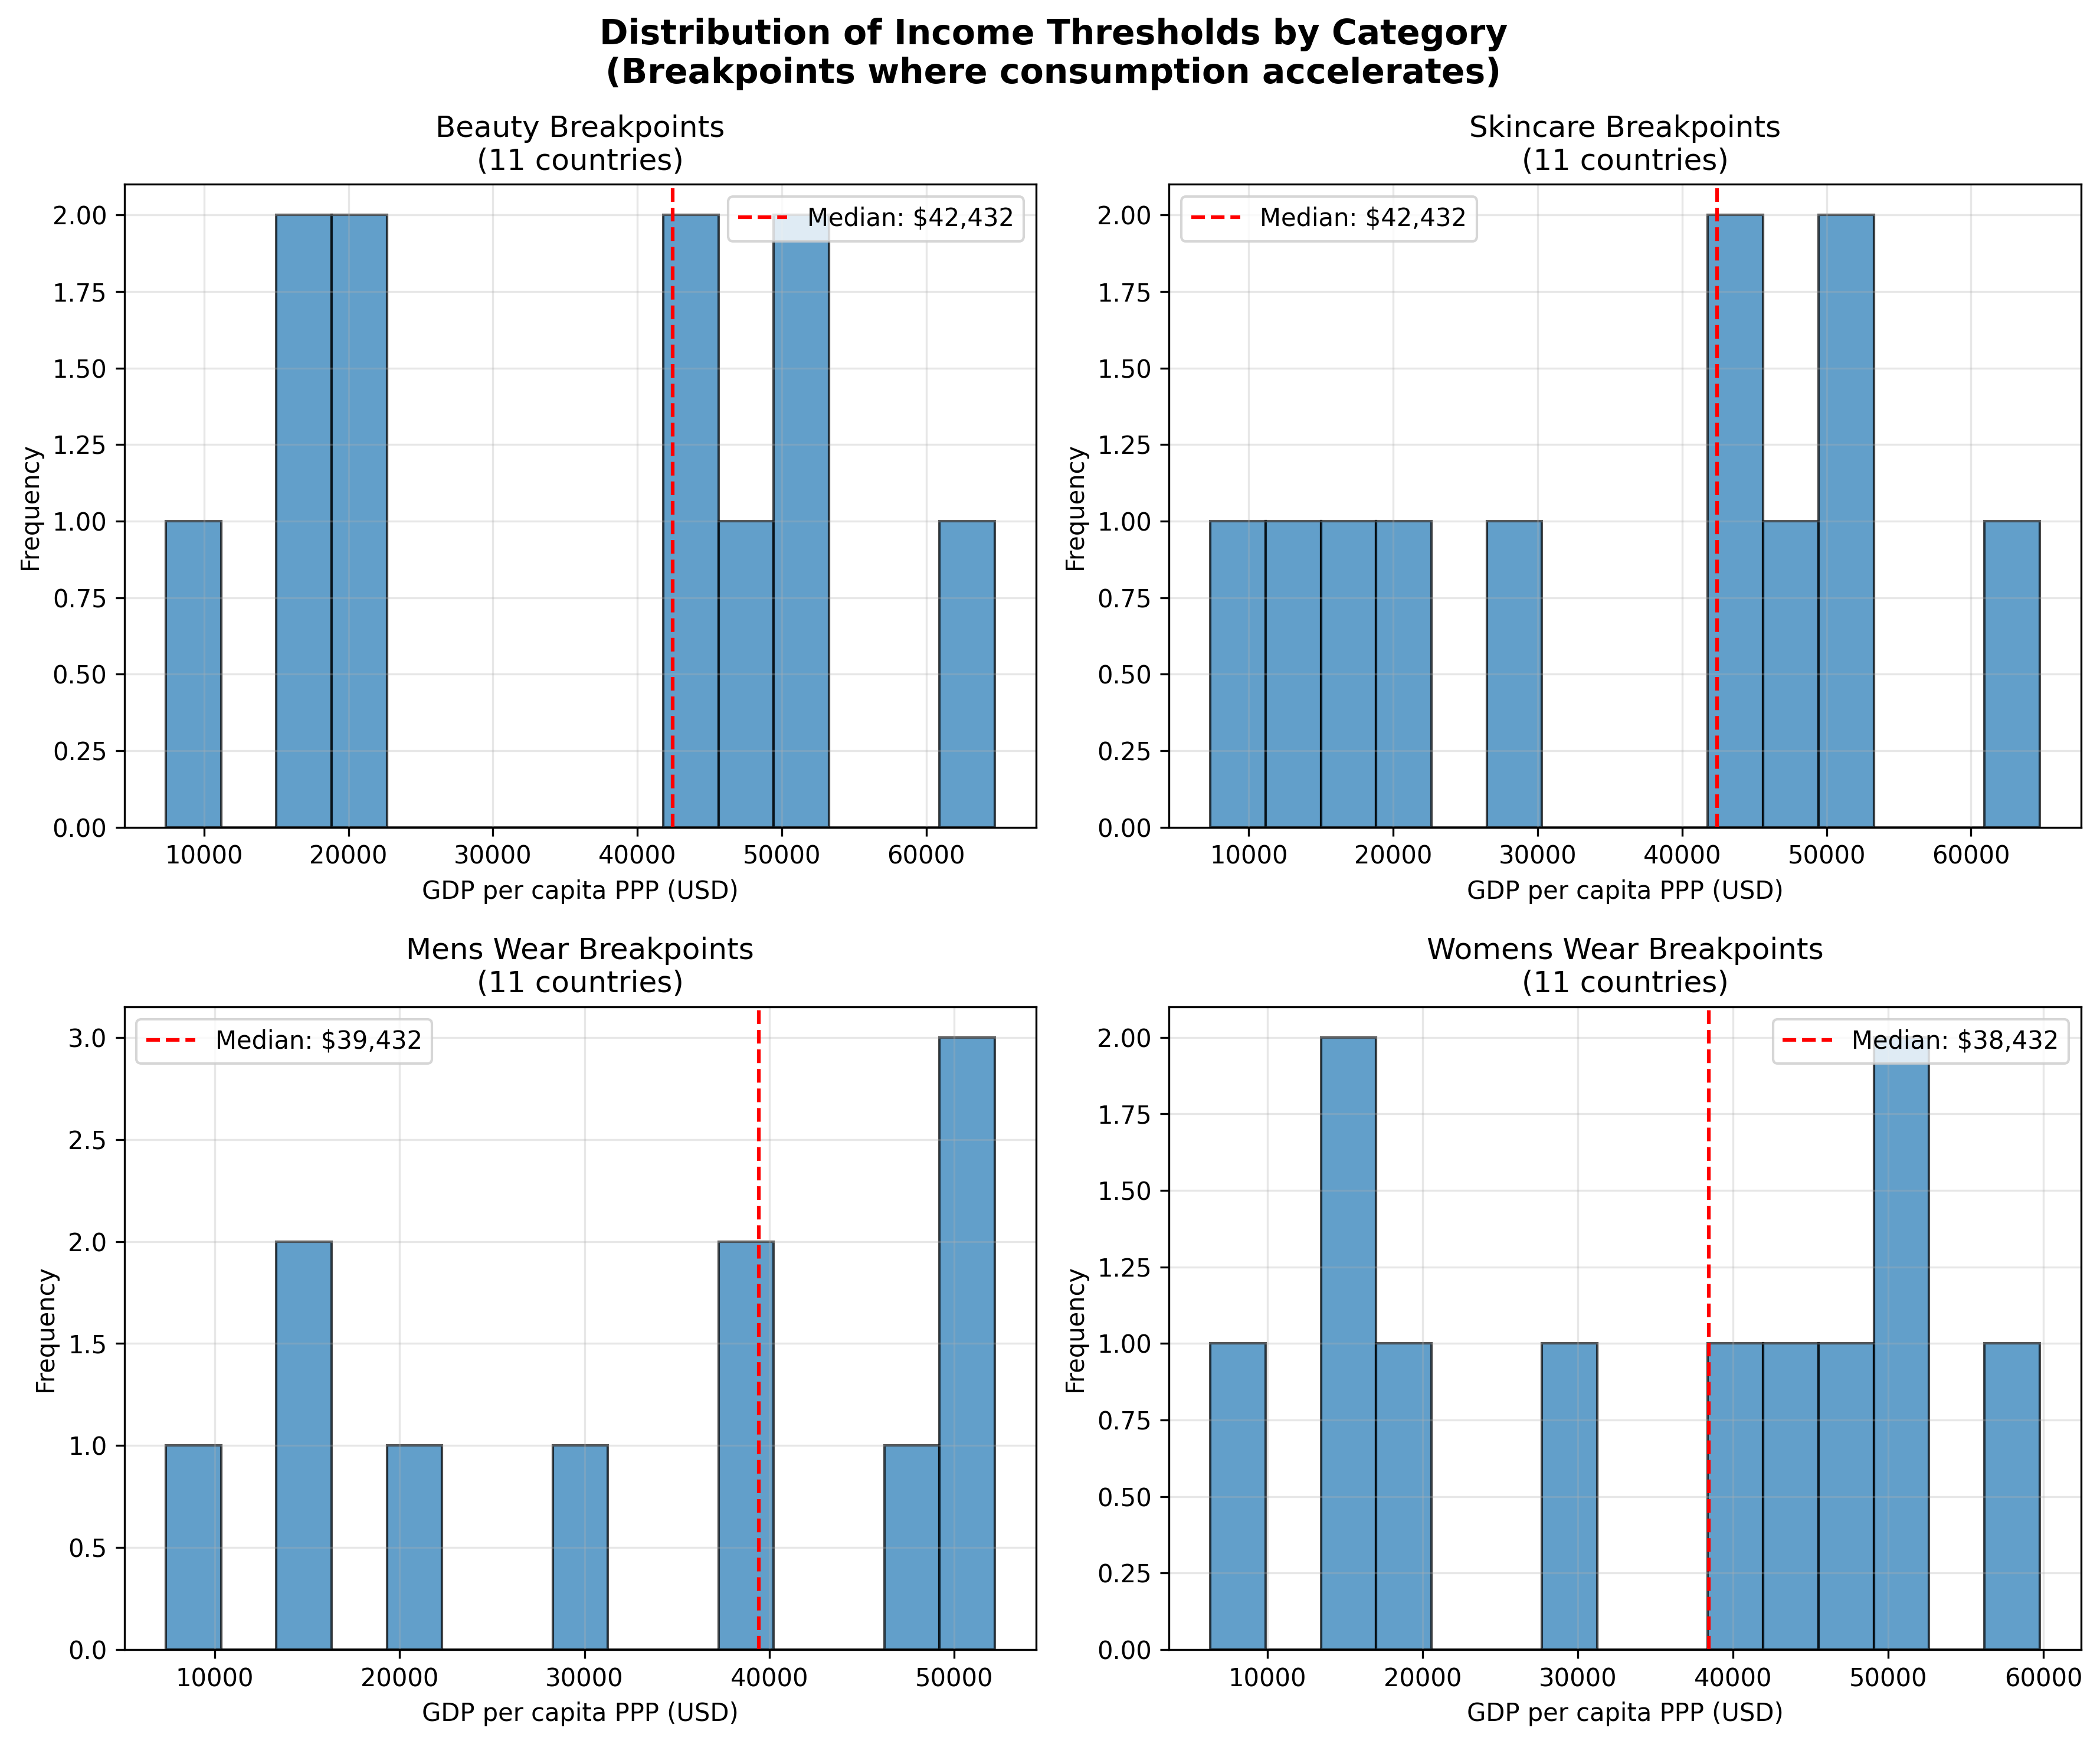
\includegraphics[width=0.8\textwidth]{HT-3_breakpoint_histogram.png}
\caption{\textbf{Figure C.1}: Threshold Distribution - Statistical distribution of identified threshold points across all categories and countries, showing concentration around \$40-50k GDP levels}
\end{figure}

\begin{figure}[H]
\centering
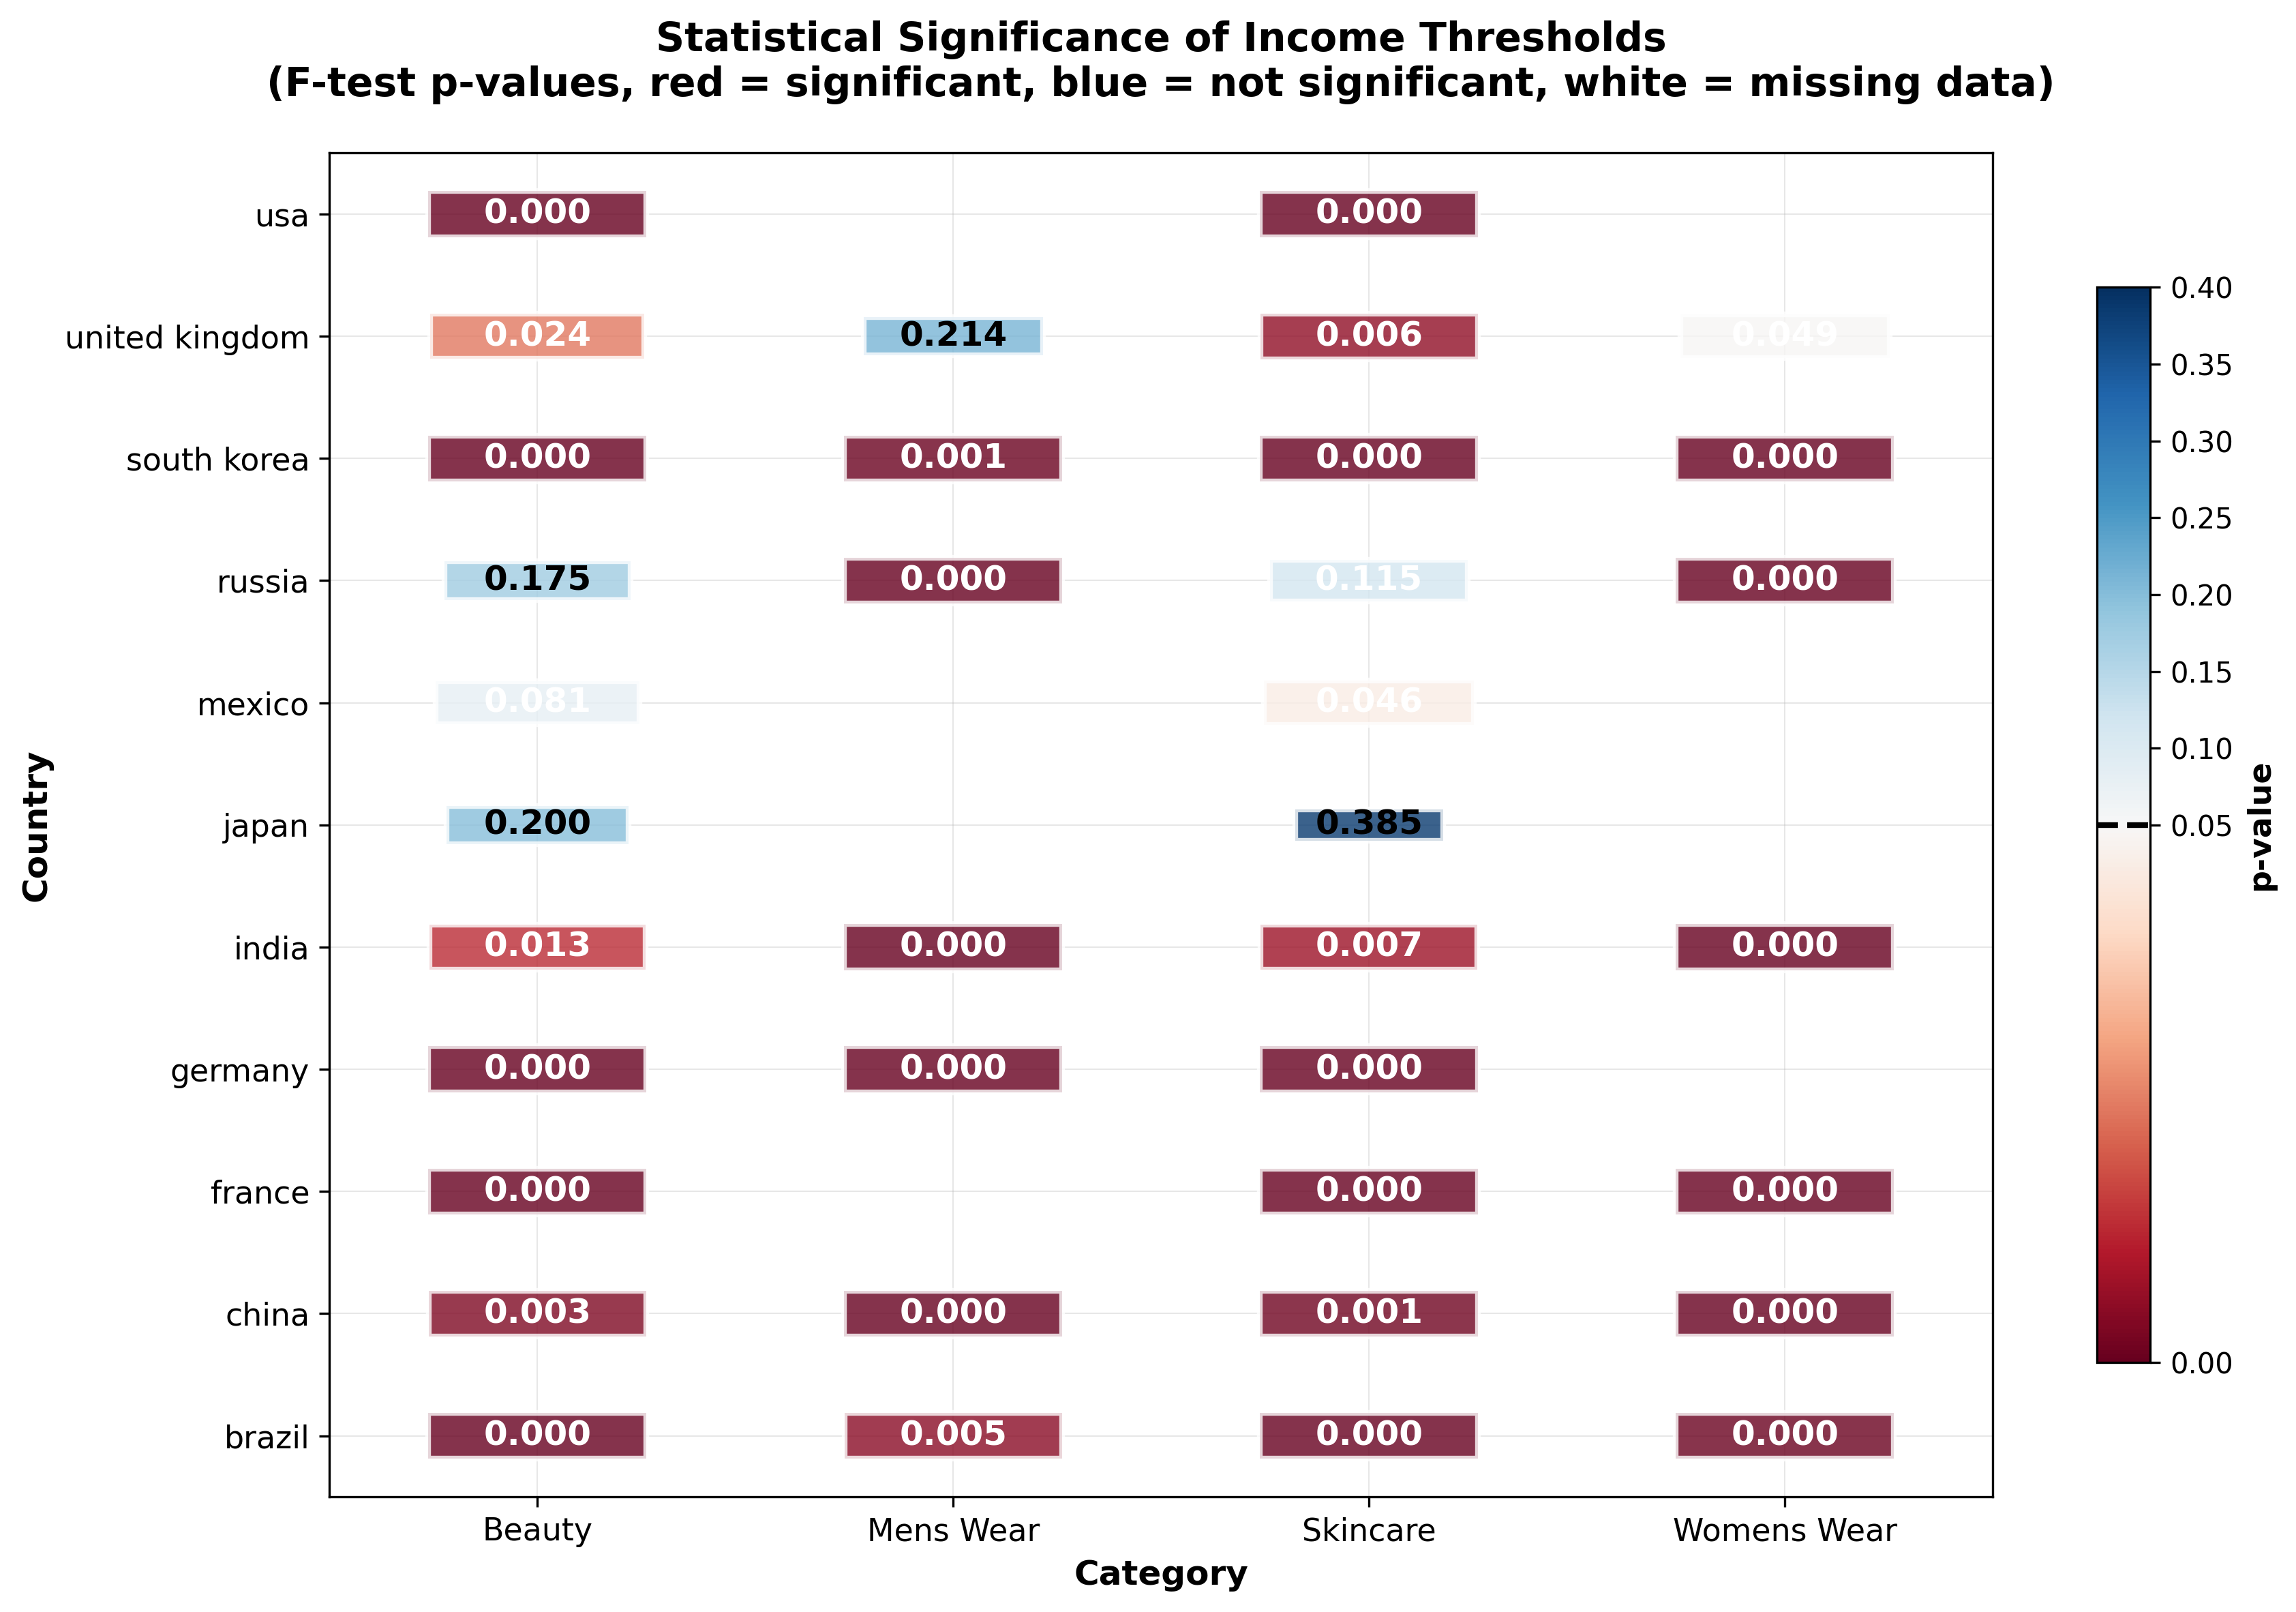
\includegraphics[width=0.8\textwidth]{HT-4_ftest_heatmap.png}
\caption{\textbf{Figure C.2}: Statistical Significance Heatmap - F-test confidence levels showing statistical significance of threshold effects across all categories and countries.}
\end{figure}

\begin{figure}[H]
\centering
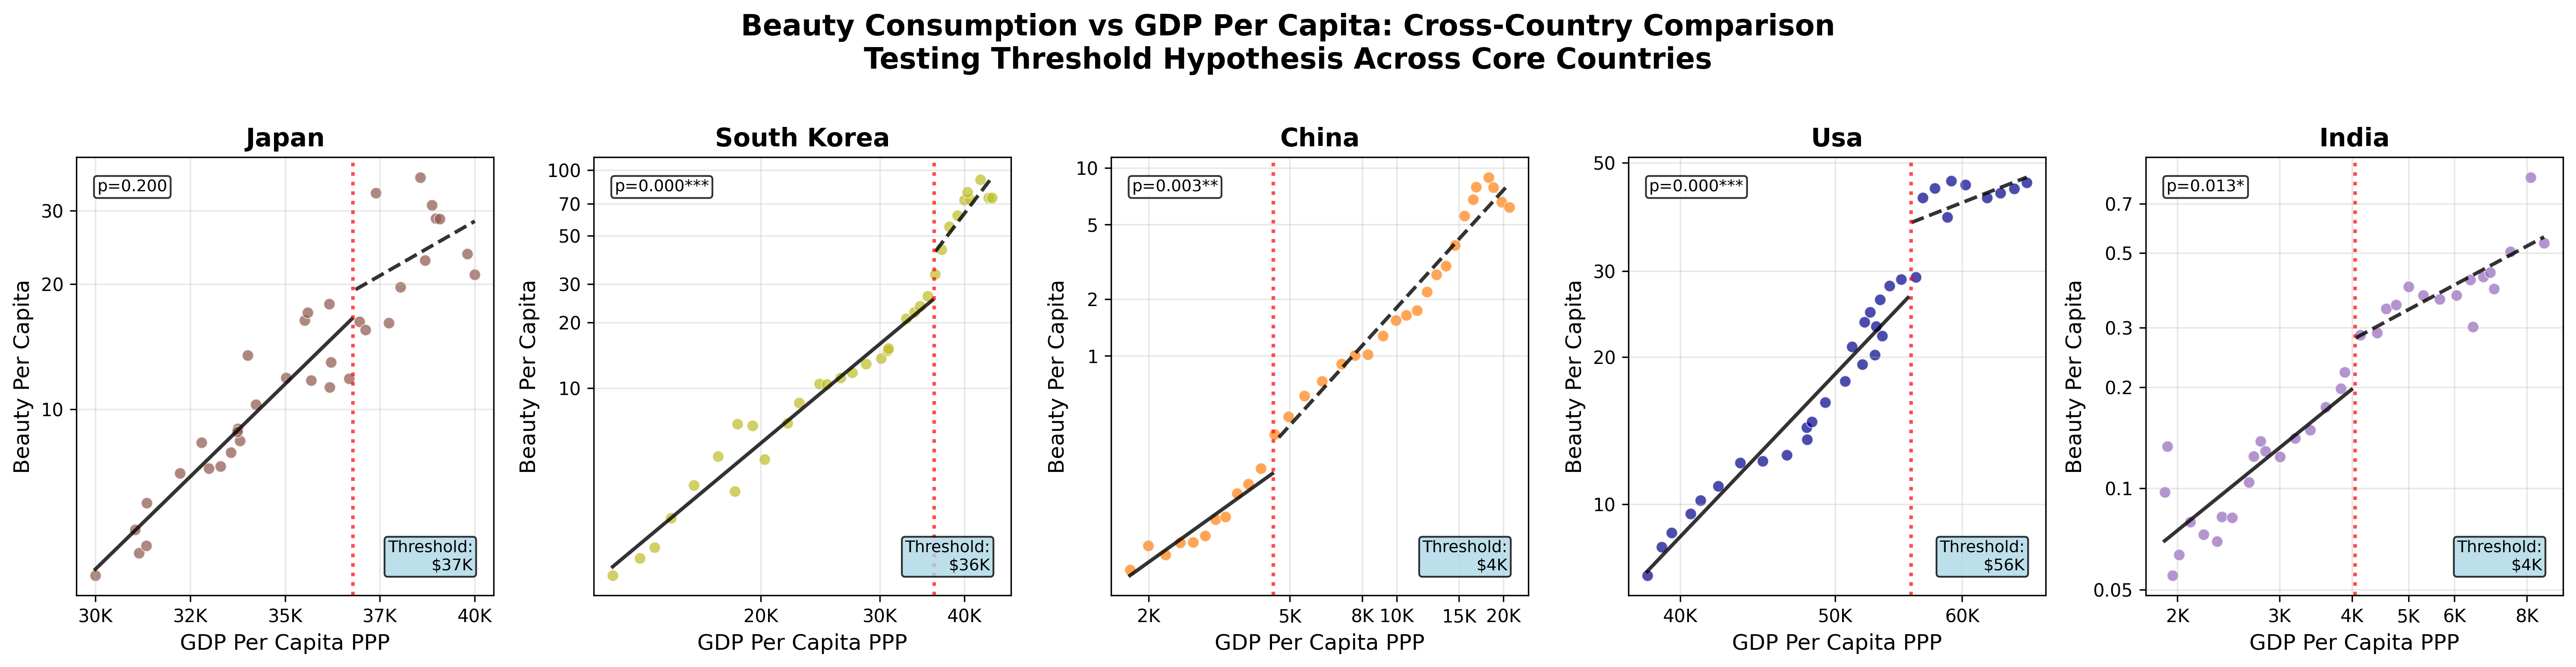
\includegraphics[width=0.8\textwidth]{HT-1_beauty_comparison.png}
\caption{\textbf{Figure C.3}: Beauty Category Comparison - Overall beauty consumption threshold analysis across all countries, demonstrating consistent acceleration patterns.}
\end{figure}

\begin{figure}[H]
\centering
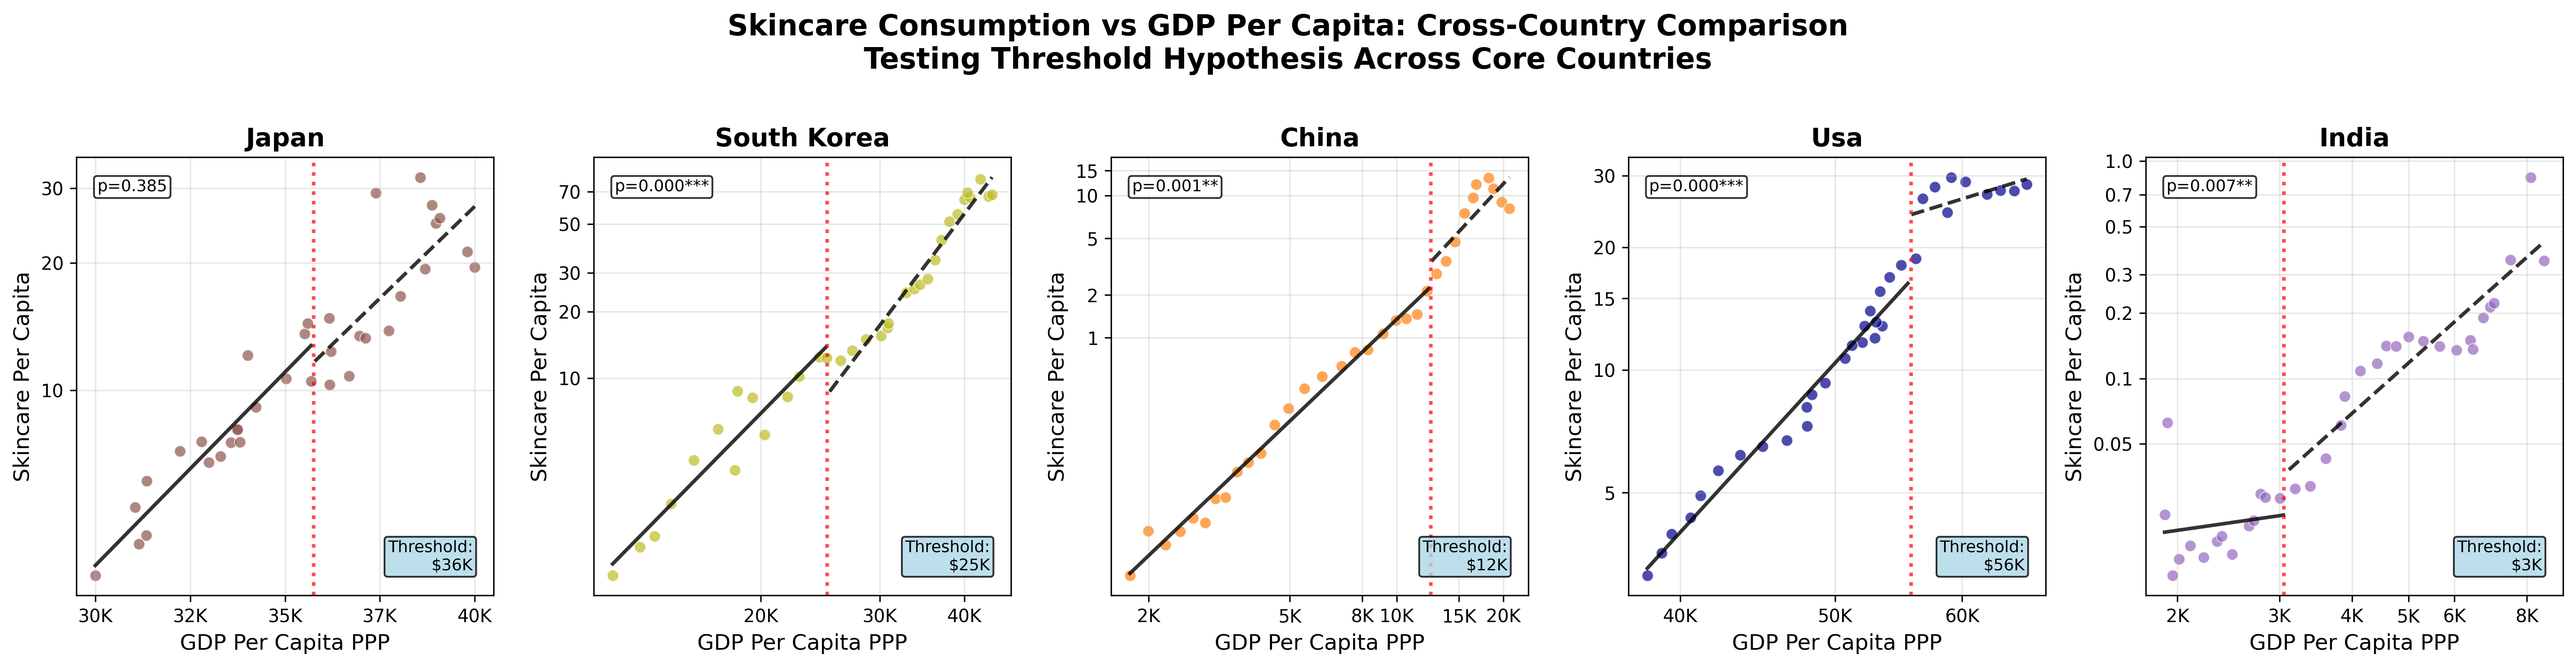
\includegraphics[width=0.8\textwidth]{HT-1_skincare_comparison.png}
\caption{\textbf{Figure C.4}: Skincare Category Analysis - Threshold effects specific to skincare products, showing strongest statistical significance across country sample.}
\end{figure}

\begin{figure}[H]
\centering
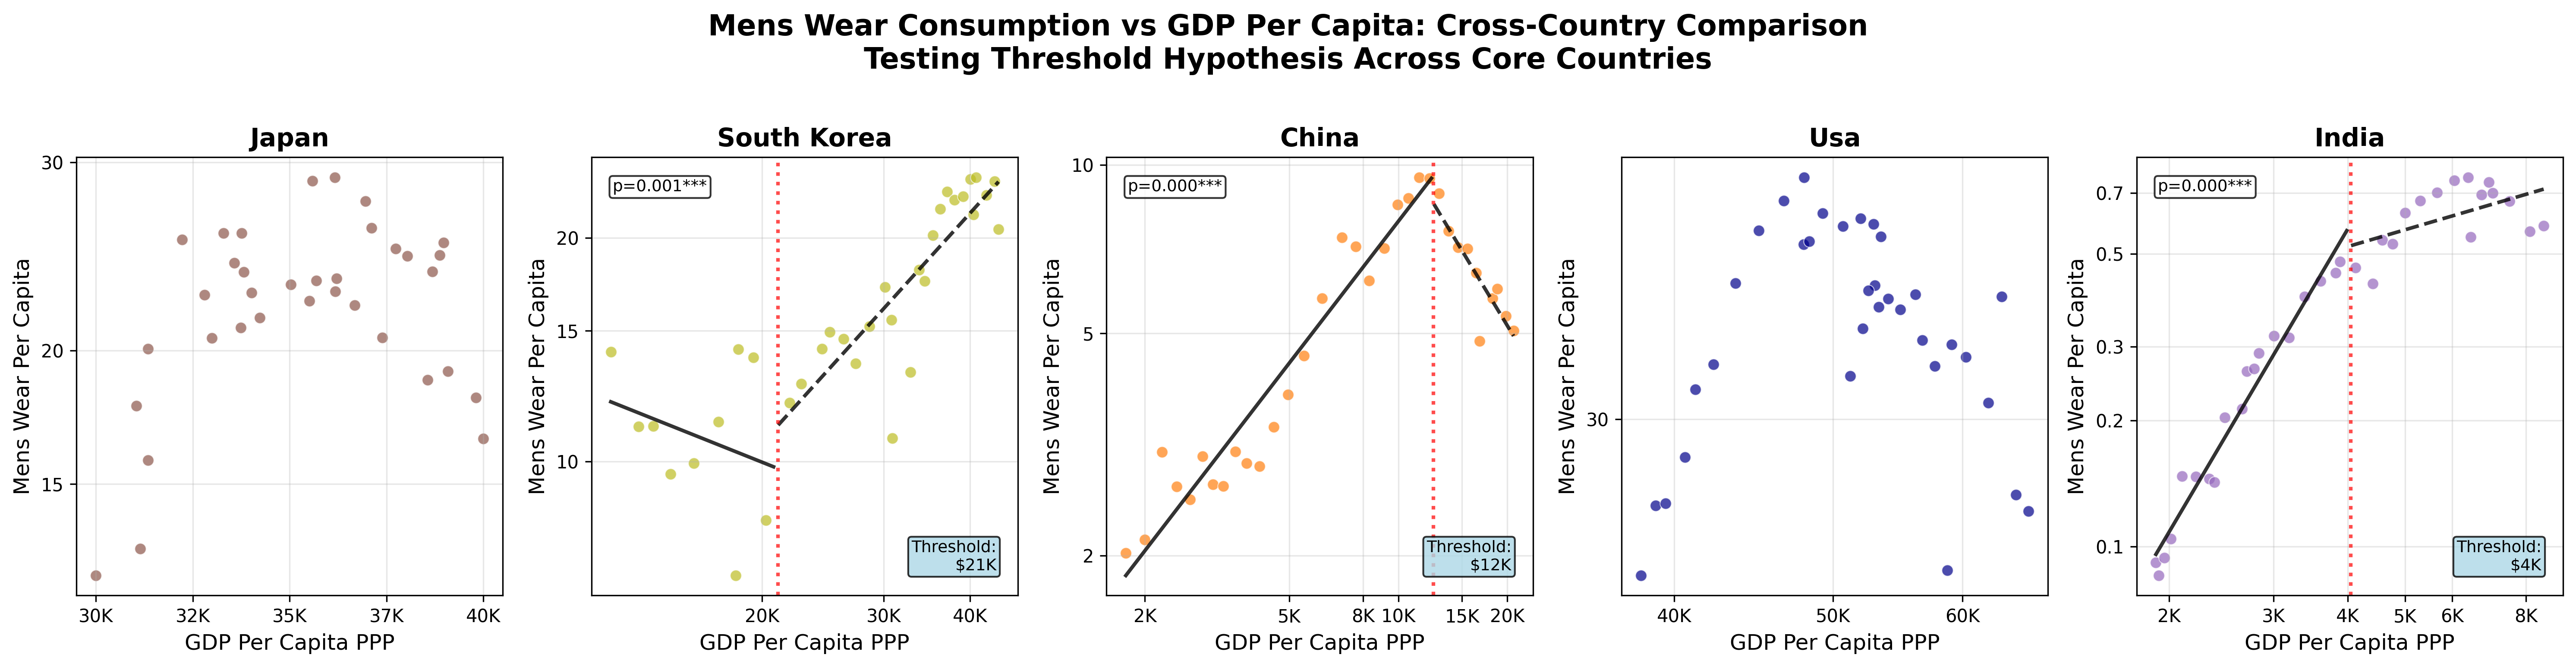
\includegraphics[width=0.8\textwidth]{HT-1_mens_wear_comparison.png}
\caption{\textbf{Figure C.5}: Men's Wear Threshold Analysis - Gender-specific consumption patterns for men's apparel, showing moderate threshold effects in select countries.}
\end{figure}

\begin{figure}[H]
\centering
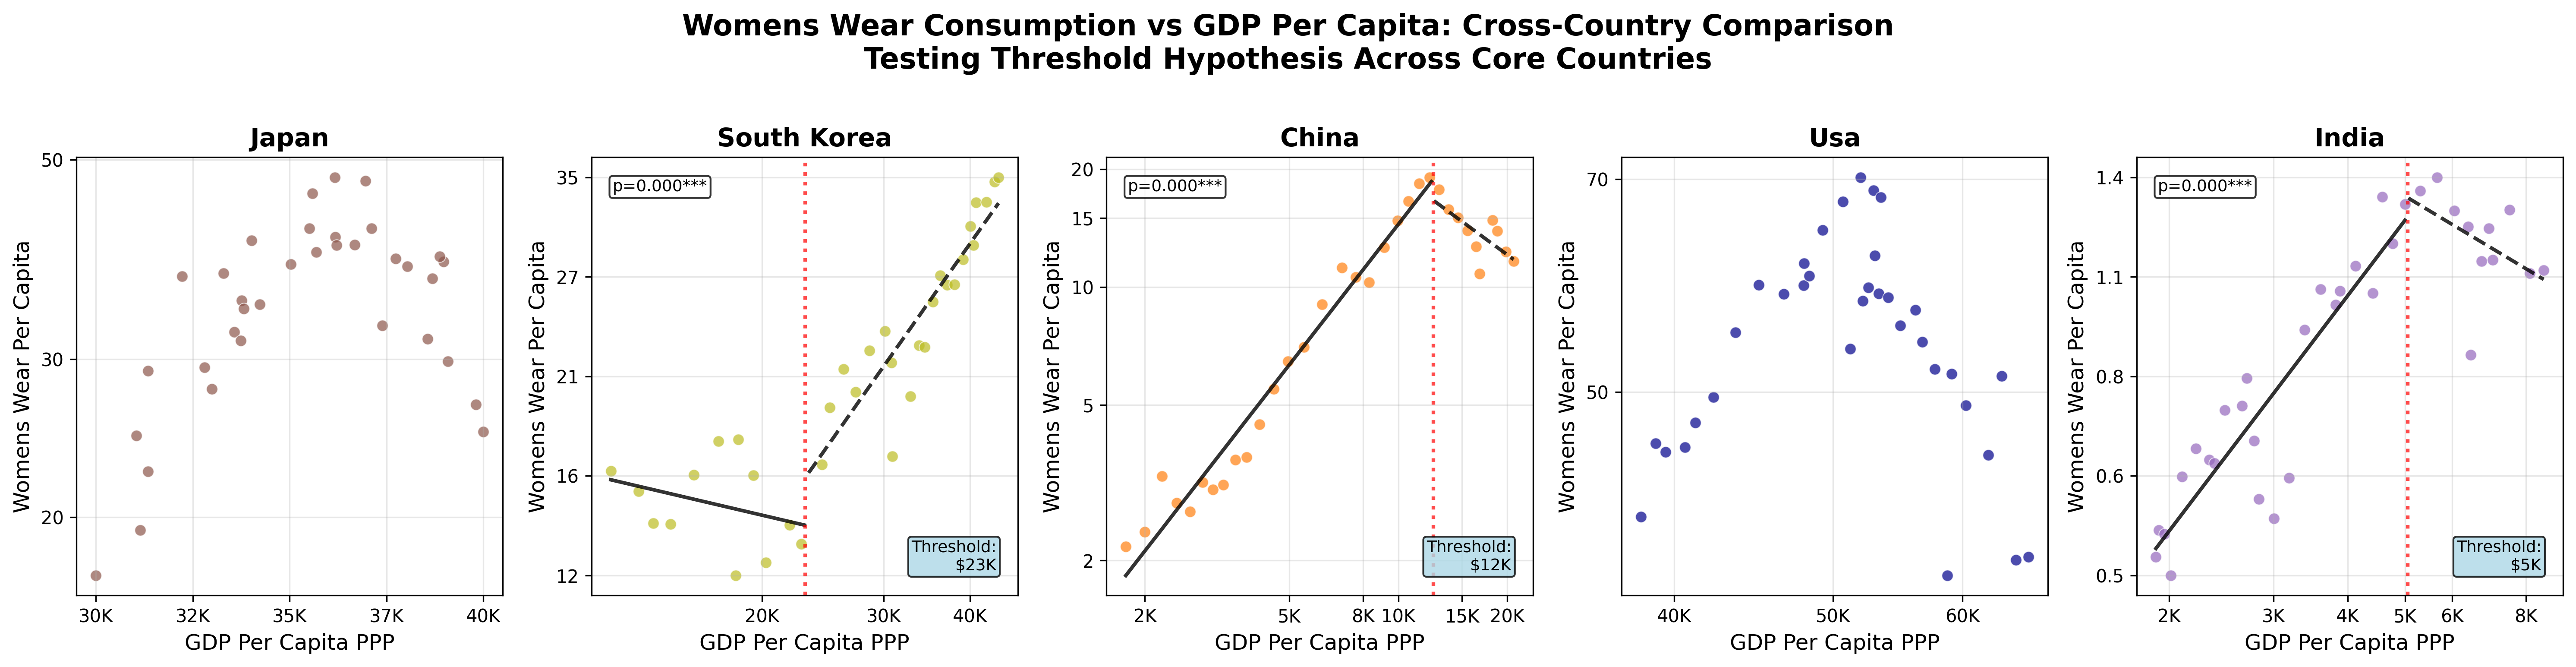
\includegraphics[width=0.8\textwidth]{HT-1_womens_wear_comparison.png}
\caption{\textbf{Figure C.6}: Women's Wear Analysis - Female apparel consumption thresholds, demonstrating strong effects in emerging markets with weaker patterns in developed countries.}
\end{figure}


\subsection*{Section E: Individual Country Analysis}

\textbf{Detailed country-specific threshold analysis providing granular evidence for hypothesis testing.}

The following individual country charts provide detailed analysis for each nation across all product categories. These charts support the aggregated findings presented in the main analysis and demonstrate the consistency of threshold effects across different economic and cultural contexts.

\textit{Individual country analysis includes 19 detailed charts covering Brazil, China, India, Japan, South Korea, and USA across beauty, skincare, men's wear, and women's wear categories. Each chart shows consumption patterns, identified thresholds, and statistical confidence intervals.}

\textit{For space considerations, individual country charts are available in digital format. Key findings from country-specific analysis are incorporated into the main report conclusions.}

\subsection*{Section F: Statistical Results Tables}

\textbf{Detailed numerical results supporting all analytical conclusions.}

\textbf{Table E.1}: Income Elasticity Coefficients by Country and Category
\textit{[Detailed elasticity coefficients, standard errors, and significance levels for all country-category combinations]}

\textbf{Table E.2}: Piecewise Regression Results  
\textit{[Threshold estimates, slope coefficients, confidence intervals, and goodness-of-fit measures for all analyses]}

\textbf{Table E.3}: F-Test Results for Threshold Significance
\textit{[F-statistics, p-values, and degrees of freedom for hypothesis testing across all categories]}

\textbf{Table E.4}: Peer Country Income-Matching Results
\textit{[GDP matching years, consumption levels, and subsequent growth rates for all peer comparisons]}

\subsection*{Section G: Data Sources \& Links}

\textbf{World Bank Data Sources:}
\begin{itemize}
    \item GDP per capita, PPP (constant 2021 international \$): \textit{[User to add World Bank link]}
    \item Household final consumption expenditure per capita (constant 2015 US\$): \textit{[User to add World Bank link]}
    \item Population, total: \textit{[User to add World Bank link]}
\end{itemize}

\textbf{UN Comtrade Data Sources:}
\begin{itemize}
    \item Beauty products (HS 3303-3307): \textit{[User to add UN Comtrade link]}
    \item Apparel categories (HS 6101-6104, 6203-6204): \textit{[User to add UN Comtrade link]}
\end{itemize}

\textbf{Data Processing Scripts:}
\begin{itemize}  
    \item Master dataset construction: \texttt{src/scripts/00\_build\_master\_dataset.py}
    \item Statistical exploration: \texttt{src/scripts/01\_task1\_statistical\_exploration.py}
    \item Comparative benchmarking: \texttt{src/scripts/02\_task2\_comparative\_benchmarking.py}
    \item Hypothesis testing: \texttt{src/scripts/03\_task3\_hypothesis\_testing.py}
\end{itemize}

\end{document}